\documentclass[11pt,twoside,a4paper,BCOR8.25mm,DIV10,headsepline,footsepline,]{scrbook}
%------------------------------------------------------------------------------
%- PAKETE
%------------------------------------------------------------------------------
	%DIN A4
		\usepackage{a4}   

	%Fancy headers
		\usepackage{fancyhdr}
	
	%Sprache einstellen (Inhaltsverzeichnis, ...)
		\usepackage[english,ngerman]{babel} %american,italian,german
	
	%Euro Zeichen
		\usepackage{eurosym}	
		
		\usepackage[bookmarks=true,
					bookmarksopen=true,
   					% Lesezeichen ausgeklappt
					bookmarksnumbered=true,
					colorlinks=true,
				   	%Einf�rbung von Links
					linkcolor=black
					% Linkfarbe: schwarz					
					]
				    % Anzeige der Kapitelzahlen am Anfang der Namen der Lesezeichen
				   {hyperref}
		
	% Vereinfachtes Eingeben von Leerschl�gen hinter Shortcut-Commands
	% Beispiel: \newcommand{\DNA}{desoxyribose nucleid acid\xspace}
		\usepackage{xspace}
	
	%Sortierte Literaturverweise
		\usepackage{cite}
	
	%Grafiken
		\usepackage{float} %Float-Handling mit Schalter H (gleiche Position wie im Skript)
		%\usepackage{flafter} %Verhindert Figuren vor ihrer ersten Referenz
		\usepackage{placeins} %Barriere f�r Float-Umgebungen erzeugen mit \FloatBarrier
	
	%Verbessertes Beschriften mir div. Optionen
		\usepackage{caption}
	
	%Zusaetzliche Symbole und Schriften (ams: american mathematical soc)
		\usepackage{amssymb}
		%\usepackage{amstext}
		%\usepackage{amsfonts}
		%\usepackage{amsbsy}
		%\usepackage{amscd}
		%\usepackage{latexsym}

	%Text Companion fonts which provide many text symbols (such as baht, bullet, copyright, musicalnote, onequarter, section, and yen) in the TS1 encoding.
		\usepackage{textcomp}
	
	%Drehen von Text, Tabellen, Seiten
		%\usepackage{rotating}
	
	%including graphics files, rotating parts of a page, and scaling parts of a page
		\usepackage{graphicx}
	
	%Nice drawing package
		%\usepackage{tikz}               
	
	%besserer eps import: \eps import ERSETZEN durch \epsfig
		\usepackage{epsf}
	
	%Farbunterst�tzung (ausserhalb der Bilder)
		\usepackage{color}
	
	%Postcript einbinden, wobei Text ersetzt werden kann
		%\usepackage{psfrag}
	
	%F�r den Index
		\usepackage{makeidx}
		\makeindex %Muss vor begin{document}, sonst passiert nix
	
	%Erleichterungen f�rs Deutsche inkl Silbentrennung
		%\usepackage{german}
	
	%Ensure minimal spacing of table cells (http://www.ctan.org/tex-archive/help/Catalogue/entries/cellspace.html)
		\usepackage{cellspace}
	
	%Direkte Eingabe von Umlauten mit Angabe von Schriftsatz
	%in Kombination mit 'german' sind jetzt � direkt erlaubt!
		\usepackage[latin1]{inputenc}
	
	%Source code Listings 
		\usepackage{listings}
	
	%Darstellung von Algorithmen
		\usepackage{algorithm}
		\usepackage{algorithmic}
	
	%Subfigures
		\usepackage{subfigure}

%-- Fieser Hack f�r Subfigures (braucht man, um lstlistings im Subfigures zu nutzen)
\newbox\subfigbox
\makeatletter
\newenvironment{subfloat}
{\def\caption##1{\gdef\subcapsave{\relax##1}}%
\let\subcapsave\@empty
\setbox\subfigbox\hbox
\bgroup}
{\egroup
\subfigure[\subcapsave]{\box\subfigbox}}
\makeatother
	
	%Automatically adds the bibliography and/or the index and/or the contents, etc., to the Table of Contents listing.
		%\usepackage[nottoc]{tocbibind} %,notlot,notlof
	
	%St Mary Road symbols for theoretical computer science.
		%\usepackage{stmaryrd}
	
	%URL Darstellung
		\usepackage{url}

	%PDF und Standard Latex Unterscheidung
		\usepackage{ifpdf} 

	%Fancy verbose environments
		\usepackage{fancyvrb}	

	%Abk�rzungsverzeichnis
		\usepackage{nomencl}
		  \let\abbrev\nomenclature
		  \renewcommand{\nomname}{Abk�rzungsverzeichnis}
		  \setlength{\nomlabelwidth}{.25\hsize}
		  \renewcommand{\nomlabel}[1]{#1 \dotfill}
		  \setlength{\nomitemsep}{-\parsep}
		  \makenomenclature

	  \newcommand{\abk}[2]{#1\abbrev{#1}{#2}}
				
	%With \usepackage{ulem}, you have the following new commands:
		%    * \uline{important} underlined text
		%    * \uuline{urgent} double-underlined text
		%    * \uwave{boat} wavy underline
		%    * \sout{wrong} line drawn through word
		%    * \xout{removed} marked over with //////.
		%    * {\em phasized\/} and \emph{asized} In LaTeX, by default, these are underlined; use \normalem or [normalem] to restore italics
		%    * \useunder{\uwave}{\bfseries}{\textbf} use wavy underline in place of bold face 
		%Note that this package changes \em and \emph to be underline. To change this behavior back to normal, use the \normalem command, for example
		%\usepackage{ulem}
		%\normalem
		%\usepackage[normalem]{ulem}

	  %\newcommand{\markup}[1]{\uline{#1}}	

	% package to customize the three basic lists (enumerate, itemize and description) 
	% by means of a set of parameters, and to clone them to define new "logical" lists.
		\usepackage{enumitem}
		\setitemize{enumsep=-3pt}
		\setitemize{itemsep=-3pt}

	%Definitionen
		\usepackage{theorem}
		\newcounter{theorem}
		\newtheorem{definition}[theorem]{Definition}

	%Zitate
		\newcounter{quotectr}
		\newtheorem{myquote}[quotectr]{Zitat}

%------------------------------------------------------------------------------
%- Layout
%------------------------------------------------------------------------------

	%Tiefe des Inhaltsverzeichnisses und der Nummerierung der Kapitel
		\setcounter{secnumdepth}{2}
		\setcounter{tocdepth}{2}

	%Call this after each chapter to avoid headlines on empty pages
		\newcommand{\chapterfin}{\clearpage{\pagestyle{empty}\cleardoublepage}}
		\newcommand{\sectionfin}{\clearpage{\pagestyle{empty}\cleardoublepage}}

	% Listings schoen machen 
		\renewcommand*\ttdefault{txtt}
	
		\lstset{%
		  breaklines=true,
		  basicstyle=\ttfamily\footnotesize,%
		  moredelim=[is][\fontseries{lt}\bfseries]{|}{|},%
		  captionpos=b,%
		  numbers=left,%
		  tabsize=1,%
		  numberstyle=\tiny,%
		  numbersep=6pt,%
		  frame=lr,%
		  framesep=0pt,%
		  framexleftmargin=5pt,%
		  framextopmargin=0pt,%
		  framexbottommargin=0pt,%
		  xleftmargin=15pt,%
		  xrightmargin=15pt,%
			abovecaptionskip=0pt,%
			belowcaptionskip=-0pt,%
		}	
		
		\lstdefinelanguage{XMLSchema}
			{morekeywords={schema,element,annotation,appinfo,complexType,simpleType,choice,all,sequence},		
			sensitive=true,
%			morecomment=[l]{//},
%			morecomment=[s]{/*}{*/},
			morestring=[b]",
		}
		
		\lstdefinelanguage{ASN1}
			{morekeywords={},		
			sensitive=true,
%			morecomment=[l]{//},
%			morecomment=[s]{/*}{*/},
			morestring=[b]",
		}
		
	
	% Font
	%
	%	Danach muss man die Standardschriftart setzen mit dem Befehl \fontfamily{abr}\selectfont, 
	% der f�r das gesamte restliche Dokument gilt, oder mit {\fontfamily{abr}\selectfont Some Text} 
	% um nur den eingeklammerten Bereich zu betreffen. abr ist die Abk�rzung f�r die Schriftart. Die 
	% h�ufigsten sind ptm (Times), phv (Helvetica), pcr (Courier), pbk (Bookman), pag (Avant Garde), 
	% ppl (Palatino), bch (Charter), pnc (New Century Schoolbook), pzc (Zapf Chancery), put (Utopia ).

	% Sch�nerer tt font:
		%\renewcommand{\ttdefault}{pcr}
		%\selectfont
	
	% Times
		%\usepackage{times}
		
	%	Helvetica
			%\usepackage{helvet}
			%\renewcommand{\familydefault}{\sfdefault}
			%\renewcommand{\familydefault}{phv}
			%\fontfamily{abr}\selectfont
			
	%	Courier
			%\usepackage{courier} \raggedright
			%\renewcommand{\familydefault}{\ttdefault}
	
	% Absatzformatierungen:
	% Keeps the distance between paragraphs constant
		\setlength{\parskip}{1.5ex plus 0.0ex minus 0.0ex}
		\setlength{\parindent}{0pt}
	
	% Modify the placement of figures: from faq source: You can adjust the cut-off value if you like, 
	% but it makes no sense to go higher than .95 (LaTeX's default value is only .5). Also, the first 
	% 3 values should be equal, and the last should be 1 - \floatpagefraction.  Otherwise, you are 
	% likely to get floats flushed to the end. 
		\renewcommand{\floatpagefraction}{0.9}
		\renewcommand{\topfraction}{0.9}
		\renewcommand{\bottomfraction}{0.9}
		\renewcommand{\textfraction}{0.1}
		\renewcommand{\textfloatsep}{5mm}
	
	% Zeilenabstand
		\renewcommand{\baselinestretch}{1.0}

	% Fancyheaders 	
		\fancyhf{} % Delete all fields
		%\fancyhead[EL,OR]{\thepage}
		\fancyhead[EL]{\nouppercase{\leftmark}}
		\fancyhead[OR]{\nouppercase{\rightmark}}
		\fancyfoot[EL,OR]{\thepage}	
		
	% Itemize look and feel
		\renewcommand{\labelitemi}{\rule[+0.9mm]{2.7pt}{2.7pt}}
		\renewcommand{\labelitemii}{--}
		%\renewcommand{\labelitemiii}{}
		%\renewcommand{\labelitemiv}{\#}	

	% Floats richtig benennen:
		%\floatname{algorithm}{Algorithm}
		%\renewcommand{\listalgorithmname}{Algorithmen}
		
%------------------------------------------------------------------------------
%- Textbausteine
%------------------------------------------------------------------------------

	%Helpers
		\newcommand{\todo}[1]				{{\em [#1]}\marginpar{{\bf [!!!]}} }
		
		\newcommand{\eigenname}[1]	{{\em #1}}
		
	%Deutsch
		\newcommand{\figref}[1]{Abbildung~\ref{fig:#1}}
		\newcommand{\tabref}[1]{Tabelle~\ref{tab:#1}}
		\newcommand{\equref}[1]{Gleichung~\ref{equ:#1}}
		\newcommand{\chapref}[1]{Kapitel~\ref{cha:#1}}
		\newcommand{\appref}[1]{Anhang~\ref{cha:#1}}
		\newcommand{\secref}[1]{Abschnitt~\ref{sec:#1}}
		\newcommand{\lstref}[1]{Listing~\ref{lst:#1}}
		\newcommand{\algref}[1]{Algorithmus~\ref{alg:#1}}
		\newcommand{\ssecref}[1]{Unterabschnitt~\ref{ssec:#1}}
		\newcommand{\quoteref}[1]{Zitat~\ref{quote:#1}}

	%Englisch	
		%\newcommand{\figref}[1]		{Figure~\ref{fig:#1}}
		%\newcommand{\tabref}[1]		{Table~\ref{tab:#1}}
		%\newcommand{\equref}[1]		{Equation~\ref{equ:#1}}
		%\newcommand{\algref}[1]		{Algorithm~\ref{alg:#1}}
		%\newcommand{\defref}[1]		{Definition~\ref{def:#1}}
		%\newcommand{\quoteref}[1]	{Quote~\ref{quote:#1}}
		
		%\newcommand{\chapref}[1]	{Chapter~\ref{cha:#1}}
		%\newcommand{\appref}[1]		{Appendix~\ref{cha:#1}}
		%\newcommand{\secref}[1]		{Section~\ref{sec:#1}}
		%\newcommand{\ssecref}[1]	{Section~\ref{ssec:#1}}
		%\newcommand{\sssecref}[1]	{Section~\ref{sssec:#1}}
		
	% REDEFINE UGLY STUFF
		\renewcommand{\leq}		{\leqslant}
		\renewcommand{\geq}		{\geqslant}
		\renewcommand{\epsilon}	{\varepsilon}
		\newcommand{\musec}		{$\mu sec$\xspace}
		\newcommand{\muW}		{$\mu W$\xspace}
		\newcommand{\plusminus}	{$\pm $\xspace}
	
%------------------------------------------------------------------------------
%- Worttrennung
%------------------------------------------------------------------------------
	
	%\hyphenation{Ge-samt-ozon}	
	\hyphenation{name-space}	
	\hyphenation{name-spaces}	
	\hyphenation{ge-samten}	
			
%------------------------------------------------------------------------------
%- Grafiken
%------------------------------------------------------------------------------

	\ifpdf
	  \DeclareGraphicsExtensions{.jpg,.pdf,.png}   % for pdftex driver
	\else
	  \DeclareGraphicsExtensions{.eps}             % for dvips driver
	\fi
	
	% Vereinfacht die Einbettung von Grafiken
	% Beispiel: \myfig[5cm]{psdatei}{�bersicht �ber das Gesamtsystem}
	\newcommand{\myfig}[3][\columnwidth]
	{
	 \begin{figure}[htbp]
		 \begin{center}
			 \includegraphics[width=#1]{img/#2}
			 \caption{#3}
			 \label{fig:#2}
		 \end{center}
	 \end{figure}
	}
	
	\newcommand{\myfigtwo}[4][\columnwidth]
	{
		 \begin{figure}[htbp]
				\begin{center}
				  \mbox
				  {
				    \subfigure[#2] 
				    { \includegraphics[width=.45\columnwidth]{img/#1-a} \label{fig:#1-a} } 
				    \quad
				    \subfigure[#3]
				    { \includegraphics[width=.45\columnwidth]{img/#1-b} \label{fig:#1-b} }
			    }
				  \caption{#4}
					\label{fig:#1}
				\end{center}
			\end{figure}
	}
	
	\newcommand{\myfigthree}[5][\columnwidth]
	{
		 \begin{figure}[htbp]
				\begin{center}
				  \mbox{
				    \subfigure[#2]
				    {
				    	\includegraphics[width=.3\columnwidth]{img/#1-a}
				    	\label{fig:#1-a}
				    } 
				    \subfigure[#3]
				    {
							\includegraphics[width=.3\columnwidth]{img/#1-b}
				    	\label{fig:#1-b}
				    }
				    \subfigure[#4]
				    {
							\includegraphics[width=.3\columnwidth]{img/#1-c}
				    	\label{fig:#1-c}
				    }
			    }	
				  \caption{#5}
					\label{fig:#1}
				\end{center}
			\end{figure}
	}
	
	\newcommand{\myfigfour}[6][\columnwidth]
	{
		 \begin{figure}[htbp]
				\begin{center}
				  \mbox
				  {
				    \subfigure[#2] 
				    { \includegraphics[width=.45\columnwidth]{img/#1-a} \label{fig:#1-a} } 
				    \quad
				    \subfigure[#3]
				    { \includegraphics[width=.45\columnwidth]{img/#1-b} \label{fig:#1-b} }
			    }
				  \mbox
				  {
				    \subfigure[#4] 
				    { \includegraphics[width=.45\columnwidth]{img/#1-c} \label{fig:#1-c} } 
				    \quad
				    \subfigure[#5]
				    { \includegraphics[width=.45\columnwidth]{img/#1-d} \label{fig:#1-d} }
			    }
			    
				  \caption{#6}
				\label{fig:#1}
				\end{center}
			\end{figure}
	}
	


% F�r das Abk�rzungsverzeichnis
\usepackage[printonlyused]{acronym}  
\usepackage{savefnmark}

% Schusterjungen und Hurenkind vermeiden
%
\clubpenalty = 10000
\widowpenalty = 10000
\displaywidowpenalty = 10000

%Um die Abkuerzungen zu ermoeglichen:
% 	makeindex.exe thesis.nlo -s nomencl.ist -o thesis.nls
%   als Postprocessor in Texniccenter einrichten

% Nette Hinweise zum LaTexen einer Diss: 
% - http://iacweb.ethz.ch/en/various/Mittelbau/disslatex.html
% - http://www.zib.de/pfetsch/Diss-Styles/
% - http://www2.informatik.hu-berlin.de/~nlohmann/arbeit/koma.html

% Hiermit kann man festlegen, dass immer nur ein bestimmter Teil �bersetzt wird
%\includeonly{1-einleitung}

\begin{document}
\selectlanguage{ngerman}
\frontmatter

%---------------------------------------------------------------------------
% Frontpage
%---------------------------------------------------------------------------
	%---------------------------------------------------------------------------
% Frontpage
%---------------------------------------------------------------------------

\begin{titlepage}

\title{Entwicklung einer Android Anwendung zum transparenten und anonymen
Sammeln von Sensordaten}
\author{Malte Legenhausen}

\let\footnotesize\small
	\let\footnoterule\relax
	\null
	\vfil
	\vskip 30pt
	\begin{center}
		{\LARGE
		  {
\includegraphics[width=80mm]{grafiken/Logo_Inst_Telematik_cropped.pdf}
			\\
			\vskip 20pt
			\Large Universit"at zu L"ubeck}\\
			Institut f"ur Telematik\\[2cm]
			{\Large Masterarbeit}\\ [2cm]
			Entwicklung einer Android Anwendung zum transparenten und anonymen Sammeln
			von Sensordaten \par}%
		\vskip 5em
		{\large \lineskip .75em
		\begin{tabular}[t]{c}
			{\Large von}\\[.5em]
			{\Large Malte Legenhausen}\\[7em]
			{\bf Aufgabenstellung und Betreuung:}\\[.5em]
			Prof.\ Dr.\ S.\ Fischer\\
			Dr.-Ing.\ Dennis\ Pfisterer\\
			M.\ Sc.\ Daniel\ Bimschas
		\end{tabular}
		\par}%
		\vfill 
		{\large
			L�beck, den \today
			\par}%
	\end{center}
	\par
	% thanks
	\vfil
	\null
\end{titlepage}

\cleardoublepage

% Erklaerung
\newpage
\vspace*{7cm}
\centerline{\bf Erkl"arung}

\vspace*{1cm}
Ich versichere, die vorliegende Arbeit selbstst"andig und nur unter Benutzung
der angegebenen Hilfsmittel angefertigt zu haben.

\vspace*{3cm}
L�beck, den \today 

\pagestyle{headings}

\cleardoublepage

% Kurzfassung und Abstract

\centerline{\bf Kurzfassung}
\bigskip
In der heutigen Zeit erfassen Smartphones sehr viele personenbezogene Daten
(z.B. Standort, Benutzerverhalten) �ber ihren Besitzer. Diese Daten besitzen
einen relativ hohen Wert f�r �ffentliche Einrichtungen und die Industrie. In den
meisten F�llen, werden diese Daten ohne das Wissen des Benutzers, aber nur an
wenige externe dritte �bertragen (z.B. Mobilfunkanbieter, Google, Apple). Die in
dieser Arbeit entwickelte L�sung, soll eine Android Anwendung darstellen, die
das transparente und anonyme Sammeln von Sensordaten erm�glicht. Die Anwendung
stellt dazu ein Erweiterungssystem bereit, das die kontrollierte Ausf�hrungs von
Plug-Ins erlaubt. Plug-Ins k�nnen von externen Einrichtung entwickelt
werden und beliebige Daten �ber den Benutzer sammeln. Der Benutzer erh�lt die
M�glichkeit zu jedem Zeitpunkt alle gesammelten Daten einzusehen und kann selbst
bestimmen welche Daten �bertragen werden sollen und welche nicht. Durch diese
Anwendung soll der Benutzer die Kontrolle �ber seine Daten wiedererlangen und es
auch anderen Instritutionen erm�glichen personenbezogene Daten zu sammeln.

%
\vskip 3cm
%

\centerline{\bf Abstract}
\bigskip
Today's smartphones collect a high amount of personalized data (e.g. position,
user behaviour) from the owner. This data has a relativly high value for public
institutions and the industry. But in most cases this data is transmitted
without the knowledge of the user only to few external thrid parties (e.g. 
provider of mobile telecom services, Google, Apple). The solution developed in
this thesis is an Android application that is able to collect personalized data
in a transparent and anonymous way. The application provides an extensible
system that allows the controlled executions of plug-ins. Plug-Ins can be
developed by external institutions that can collect arbitary data about the
user. At any point in time the user has the possibility to review all
the collected data and can decide which data is transfered and which not.
Through this application the user should get back control over his data and
enable other institutions to collect personalized data.

\cleardoublepage

%---------------------------------------------------------------------------
% Inhaltsverzeichnis
%---------------------------------------------------------------------------
	\tableofcontents
	\cleardoublepage

%---------------------------------------------------------------------------
% Der eigentliche Inhalt
%---------------------------------------------------------------------------
	\mainmatter
	\pagestyle{fancy}
	
	\chapter{Einleitung}
\label{cha:einleitung}
Diese Masterarbeit�stellt die Abschlussarbeit des�Autors zum Master of Science
dar, die im�Rahmen�des�Studienganges�Informatik an�der Universit�t zu L�beck
absolviert wurde.�Die Themenbearbeitung�fand�an der Universit�t zu L�beck im
\acf{itm}�statt. Der�Themenschwerpunkt�dieser Masterarbeit�ist�die Entwicklung
einer Android Anwendung zum transparenten und anonymen Sammeln von Sensordaten.

Diese Anwendung soll einige Nachteile der bisherigen Ans�tze der mobilen
Datenerfassung l�sen, die auf potenziell pers�nliche Daten eines Smartphone-Benutzers
zugreifen. Denn heutzutage werden �ber einen Benutzer, eine
Vielzahl unterschiedlicher Daten gesammelt. Dies reicht von der aktuellen Position, bis
hin zu den Gewohnheiten wie ein Benutzer sein Smartphone verwendet. In vielen
F�llen wei� ein Smartphone-Benutzer nicht, welche Anwendung welche Daten �ber
ihn sammelt bzw. dass dies �berhaupt geschieht. Auch fehlt eine M�glichkeit die
gesammelten Daten einzusehen, geschweige denn einer �bertragung der Daten zu
widersprechen. Ob bei der �bertragung eine Anonymisierung der Daten
stattfindet, liegt ebenfalls in der Hand des Anwendungsherstellers.

Diese Umst�nde f�hren dazu, dass sich viele Smartphone-Benutzer ihrer Daten
entmachtet f�hlen und somit das Misstrauen in Anwendungen der mobilen
Datenerfassung steigt. Dies kann zu einem Problem werden, wenn immer weniger
Benutzer Daten (ob personenbezogenen oder nicht) freigeben wollen,
obwohl der Bedarf nach solchen Daten in einer Vielzahl von Industrie und
Forschungsprojekten steigt.

Motivation ist es daher, eine vertrauensw�rdige Plattform zu schaffen, auf der
aufbauend andere Institutionen Anwendungen zum Sammeln von Sensordaten
entwickeln k�nnen. Sensordaten sind im Rahmen dieser Arbeit z.~B. der L�rmpegel
der Umgebung, die aktuelle Position, die verf�gbaren Netzwerkverbindungen oder
die Daten des Beschleunigungssensors. Die Plattform soll dabei dem Benutzer
erm�glichen selbst zu entscheiden, wann welche Daten �ber ihn gesammelt werden
sollen. Transparenz soll der Benutzer dadurch erhalten, dass er zu jedem Zeitpunkt
einsehen kann, welche Daten �ber ihn gesammelt wurden. Des Weiteren soll der
Benutzer auch entscheiden k�nnen, ob die gesammelten Daten �berhaupt an eine andere
Institution freigegeben werden sollen. Anonymit�t soll dadurch erreicht
werden, dass der Zugriff auf eindeutige Benutzerdaten geregelt wird. Diese Daten
k�nnen z.~B. der Name, Telefonnummer oder die Adresse sein.

Ziel ist es die informationelle Selbstbestimmung des Benutzers zu festigen und
somit, auch das Vertrauen in die mobile Datenerfassung zu steigern. Durch dieses
Vertrauen sollen gerade �ffentliche Forschungseinrichtungen die M�glichkeit
erhalten personenbezogene Daten zu sammeln, die z.~B. im Bereich der
St�dte- und Verkehrsplanung neue Erkenntnisse liefern k�nnen.

\section{Verwandte Arbeiten}
Im Folgenden sollen auf �hnliche Arbeiten eingegangen werden, die bereits
einzelne Aspekte der zu entwickelnden Anwendung realisiert haben. 

\subsection{Sensorly}
Bei {\em Sensorly} handelt es sich um eine Android Anwendung, mit der die
Netzwerkabdeckung von Mobilfunknetzen mithilfe von Android-Smartphones ermittelt
wird. Dazu l�dt man sich als Benutzer eine Gratisanwendung aus dem {\em
Android Market} herunter und installiert diese. Nach dem ersten Start sammelt
die Anwendung automatisch im Hintergrund Daten �ber die Netzabdeckung vom gerade
verbundenen Mobilfunkanbieter. Diese Daten werden in regelm��igen Abst�nden an einen
zentralen Server �bermittelt, wo diese Daten mit den Daten anderer Anwender
kombiniert werden, um die Daten anschlie�end in einer Karte auf der
Internetseite \url{sensorly.com} zu visualisieren.

{\em Sensorly} repr�sentiert einen m�glichen Anwendungsfall f�r die zu
entwickelnde Anwendung. Es ist mit {\em Sensorly} aber nicht m�glich die Daten
vor der �bertragung einzusehen oder dieser �bertragung zu widersprechen. {\em
Sensorly} stellt also eine klassische Anwendung zum Sammeln von Sensordaten dar.

\subsection{Flexible Android Permissions}
\acf{flexp} ist eine Anpassung des Android Betriebssystems, die es erm�glicht,
die Rechte die einer Anwendung bei der Installation gegeben werden, nachtr�glich zu
ver�ndern. Ein Benutzer hat also die M�glichkeit nachtr�glich zu bestimmen, auf
welche Ressourcen eine Anwendungen zugreifen darf und auf welche nicht. Um nun
m�gliche Probleme zu vermeiden, die nach dem Rechteentzug auftreten
k�nnen, wird den Anwendungen suggeriert, dass sie trotzdem Zugriff auf die
Ressourcen haben~\cite{flexp}.

\acs{flexp} deckt den Aspekt ab, dass durch diese Anpassung der Benutzer mehr
M�glichkeiten hat, zu entscheiden auf welche Ressourcen (z.~B. die Sensorik),
die Anwendung zugreifen darf. Der Benutzer hat aber hier ebenfalls nicht die
M�glichkeit einsehen, was passiert, wenn ein Recht trotzdem vergeben wurde. Die
Kontrollm�glichkeiten �ber eine Anwendung steigen zwar, die Transparenz bleibt
aber dieselbe.

\subsection{iPhone Tracker}
Der {\em iPhone Tracker} erlaubt die Visualisierung von Daten auf dem Computer,
die durch das Smartphone-Betriebssystem iOS auf dem Apple iPhone erhoben
werden~\cite{iphonetracker}. Diese Daten werden laut Apple dazu verwendet, die
Lokalisierung des Benutzers zu beschleunigen. Die Daten erlauben aber die
einfache Generierung von Bewegungsprofilen. Eine Einsicht dieser Daten ohne
spezielle Programme ist aber nicht m�glich~\cite{applegps}.

Der Fall des {\em iPhone Tracker} zeigt, die Problematik bei fehlender
Transparenz. Dem Benutzer ist nicht bewusst, welche Daten �ber ihn gesammelt
werden. Kommt dieses zutage, bedeutet dies oft ein Vertrauensbruch mit dem
Benutzer. Die zu entwickelnde Anwendung soll nun diese Transparenz als
Standardfunktionalit�t liefern. Anwendungen, die auf dieser aufbauen, m�ssen
sich nur um das eigentliche Sammeln von Daten k�mmern.

\section{Aufbau der Masterarbeit}
Diese Masterarbeit gliedert sich in die folgenden Kapitel:

\begin{itemize}
  \item In der {\bf Anforderungsanalyse} wird die Aufgabenstellung in ihre
  einzelnen Bestandteile zerlegt und Begrifflichkeiten gekl�rt. Dies erlaubt in
  den nachfolgenden Kapiteln die Bearbeitung der in der Aufgabenstellung
  enthaltenden Anforderungen.
  \item Die {\bf Grundlagen} befassen sich mit den verwendeten Technologien.
  Dieses Kapitel besch�ftigt sich zu einem gro�en Teil mit der Android
  Plattform.
  \item Die {\bf Konzeption} beschreibt einen weitestgehenden
  techno\-logie\-unab\-h�n\-gigen Aufbau der Anwendung. Dabei werden die
  Anforderungen in eine Architektur �berf�hrt. Es wird aber auch gekl�rt, ob die
  in den Grundlagen erw�hnten Technologien sich tats�chlich zur Realisierung
  verwenden lassen.
  \item In der {\bf Realisierung} wird die entwickelte Anwendung vorgestellt.
  Dies schlie�t interne Abl�ufe ein, wie auch die Pr�sentation der
  Benutzerschnittstelle.
  \item Der {\bf Leitfaden} dient Entwicklern als Anleitung um ihre Anwendungen
  (Plug-Ins) zu entwickeln und diese auf der Plattform auszuf�hren.
  \item Die {\bf Evaluation} dient als Best�tigung, dass die entwickelte
  Anwendung auch in realen Anwendungsszenarien einsetzbar ist.
  \item Im Kapitel {\bf Zusammenfassung und Ausblick} werden die Ergebnisse der
  Arbeit zusammengefasst und ein abschlie�endes Fazit gegeben.
\end{itemize} 	
	\chapterfin
	\chapter{Anforderungsanalyse}
\label{cha:anforderungsanalyse}
In diesem Kapitel werden die aus der Aufgabenstellung sich ergebenen
Anforderungen genauer analysiert. Es wird dabei gekl�rt, in welchem Umfang die
einzelnen Anforderungen bearbeitet werden m�ssen.

Die sich aus der Aufgabenstellung ergeben Anforderungen sind Transparenz,
Anonymit�t, ein Erweitungssystem, die m�glichkeit der Datenspeicherung, sowie
die regelm��ige �bertragung von Daten an einen Server.

\section{Transparenz}


\section{Anonymit�t}
Anonymit�t beschreibt den Zustand, einer Person oder Gruppe die
nicht identifiziert werden kann. Bei der Art von Anonymit�t
gibt unterscheidet man verschiedene Abstufungen~\cite{anonymitaet}:
\begin{itemize}
  \item formal anonym: Eindeutige Zuordnungsmerkmale (z.B. Namen usw.) sind
  entfernt, die Daten ansonsten unver�ndert (das hei�t leichte Zuordbarkeit der Einheiten).
  \item faktisch anonym: Daten sind nur nur mit unverh�ltnism��igem Zeit- und
  Arbeitsaufwand zuordbar.
  \item komplett anonym: die Zuordnung zu einzelnen Personen ist ausgeschlossen.
\end{itemize}

Im Rahmen der Aufgabenstellung soll eine Anonymisierung der Benutzers
von ``formal anonym'' bis ``faktisch anonym'' erm�glicht werden. Dies bdeutet,
dass es nicht m�glich sein soll, eindeutige Merkmale eines Benutzers zu sammeln (z.B.
IMEI, Telefonnummer) und zum anderen, eine Zuordnung zu realen Personen anhand
der Daten erschwert wird.

Bei der Anonymisierung der Daten ergibt sich aber ein Problem, bei der
zurordbarkeit von einzelnen Datens�tzen, die in regelm��igen Abst�nden an einen
Server �bertragen werden. Werden zwei Datens�tze A und B zu zwei
unterschiedlichen Zeitpunkten �bertragen, ist es nicht m�glich die
Datens�tze A und B einander zuzurodnen. Eine Zuordnung auf dieser Ebene gef�hrte
aber nicht die Anonymit�t der Benutzers. Hierbei ergibt sich nun die Anforderung
eine Verfahren zu entwickeln, dass dieses Problem l�st.

\section{Erweiterungssystem}
Aus der Aufgabenstellung ist zu entnehmen, dass die zu entwickelnde Anwendung,
nur ein Grundger�st darstellen soll. Es soll sich durch Erweitungen erweitern
lassen. Die Anforderung besteht also darin, ein bestehendes Erweitungssystem in
Android zu integrieren, oder ein eigenes zu implementieren.

Anforderungen an das Erweiterungssystem:

\begin{itemize}
  \item Der Benutzer soll die m�glichkeit haben neue Erweiterungen zu
  installieren und zu deinstallieren.
   \item Die Installation neuer Erweiterungen, soll f�r den Benutzer der
   Anwendung m�glichst einfach sein z.B. durch die Bereitstellung eines Markets.
  \item Das Erweiterungssystem soll eine Bibliothek liefern, �ber die es m�glich
  ist neue Erweiterungen m�glichst einfach zu erstellen.
\end{itemize}

\section{Datenspeicherung}
Die von den Erweiterungen gesammelten Daten m�ssen auf dem Ger�t zwischen
gespeichert werden, bevor diese �bertragen werden d�rfen. Der Benutzer soll
n�mlich die M�glichkeit besitzen, sich die gesammelten Daten, vor einer
�bertragung zu kontrollieren. Deswegen ist ein Datenmodell zu entwickeln, dass
es erm�glicht, Daten von beliebigen Erweiterungen zu speichern. Der Entwickler
einer Erweiterung soll dabei aber so wenig wie m�glich bei der Wahl seines
Datenmodell eingeschr�nkt werden.

\section{Daten�bertragung}
Die von den Erweiterungen gesammelten Daten sollen in regelm��igen Abst�nden, an
einen Server �bertragen werden. Dies soll aber nicht automatisch geschehen,
sondern es soll der Benutzer darauf hingewiesen werden, das neue Daten zur
�bermittung bereit stehen. Dadurch soll der Benutzer die m�glichkeit haben vor
einer �bertragung die Daten zu kontrollen. Ist ein Benutzer nicht mit der
�bertragung der Daten einverstanden, so soll diese �bertragung verworfen werden
k�nnen. Des Weiteren soll die M�glichkeit bestehen die �bertragung zu einem
sp�teren Zeitpunkt auszuf�hren. Dies kann der Fall sein, wenn eine �bertragung
z.B. �ber das Mobilfunknetz f�r den Benutzer zu kostenintensiv ist.

F�r die �bertragung der Daten ist ein entsprechendes Datenformat und
�bertragungsprotokoll zu w�hlen. Beim Datenformat ist darauf zu achten ein
Format zu w�hlen, dass einen geringen Overhead aufweist, da die Bandbreite im
mobilen Bereich stark limitiert ist.

Zum Empfangen der Daten ist eine entsprechende Serverkomponente zu entwickeln.
Neben dem Empfang soll die Serverkomponente es erlaubt die empfangenen Daten
weiter zu verarbeiten um sie z.B. in einer Datenbank zu speichern.

	\chapterfin
	\chapter{Verwandte Arbeiten}
\label{cha:relatedwork}
Im Folgenden soll auf Arbeiten eingegangen werden, die bereits
einzelne Aspekte der zu entwickelnden Anwendung realisiert haben. 

\section{Sensorly}
Bei {\em Sensorly} handelt es sich um eine Android-Anwendung, mit der die
Netzwerkabdeckung von Mobilfunknetzen mithilfe von Android-Smartphones ermittelt
wird. Dazu l�dt man sich als Benutzer eine Gratisanwendung aus dem {\em
Android Market} herunter und installiert diese. Nach dem ersten Start sammelt
die Anwendung automatisch im Hintergrund Daten �ber die Netzabdeckung vom gerade
verbundenen Mobilfunkanbieter. Die Daten werden in regelm��igen Abst�nden an
einen zentralen Server �bermittelt, auf dem diese mit den Daten anderer Anwender
kombiniert werden. Auf der Internetseite \url{sensorly.com} werden die
gesammelten Daten auf einer Karte �bersichtlich visualisieren.

{\em Sensorly} repr�sentiert einen Anwendungsfall f�r die zu
entwickelnde Anwendung. Es ist mit {\em Sensorly} aber nicht m�glich die Daten
vor der �bertragung einzusehen oder der �bertragung zu widersprechen. {\em
Sensorly} stellt also eine klassische Anwendung zum Sammeln von Sensordaten dar.

\section{Flexible Android Permissions}
{\em \acf{flexp}} ist eine Anpassung des Android-Betriebs\-systems, die es
erm�glicht, die Rechte, die einer Anwendung bei der Installation gegeben werden,
nachtr�glich zu ver�ndern. Ein Benutzer hat also die M�glichkeit nachtr�glich zu bestimmen, auf
welche Ressourcen eine Anwendungen zugreifen darf und auf welche nicht. Um
m�gliche Probleme, die nach dem Rechteentzug auftreten
k�nnen, zu vermeiden, wird den Anwendungen suggeriert, dass sie Zugriff
auf die Ressourcen haben~\cite{flexp}.

Durch die Anpassung, welche {\em \acf{flexp}} erm�glicht, hat der Besitzer
bessere M�glichkeiten, zu entscheiden, auf welche Ressourcen (z.B. die Sensorik)
die Anwendung zugreifen darf. Dennoch hat der Nutzer -- wie auch bei {\em
Sensorly} -- nicht die M�glichkeit, einzusehen, was passiert, wenn ein Recht
trotzdem vergeben wurde. Die Kontrollm�glichkeiten �ber eine Anwendung steigen
zwar, eine vollst�ndige Transparenz ist aber noch immer nicht gegeben.

\section{iPhone Tracker}
Der {\em iPhone Tracker} erlaubt die Visualisierung von Daten auf einem
Desktop-Computer, die durch das Smartphone-Betriebssystem iOS auf dem Apple
iPhone erhoben werden~\cite{iphonetracker}. Bei diesen Daten handelt es sich um
detailierte Informationen �ber das Mobilfunknetz und in der Umgebung befindliche
\acs{wlan}-Zugangspunkte. Diese Daten werden laut Apple dazu verwendet, die
Lokalisierung des Benutzers zu beschleunigen. Im Gegenzug erlauben die Daten
aber die einfache Generierung von Bewegungsprofilen. Eine Einsicht der Daten
ohne spezielle Programme ist nicht m�glich~\cite{applegps}.

Der Fall des {\em iPhone Tracker} zeigt die Problematik bei fehlender
Transparenz: Dem Benutzer ist nicht bewusst, welche Daten �ber ihn gesammelt
werden. Kommt dies zutage, bedeutet das oft einen Vertrauensbruch mit dem
Benutzer. Aus diesem Grund soll die zu entwickelnde Anwendung dagegen
Transparenz als Standardfunktionalit�t bieten.
	\chapterfin
	\chapter{Grundlagen}
\label{cha:grundlagen}
In diesem Kapitel wird auf die grundlegenden Technologien eingegangen, die zur
Realisierung der Anwendung verwendet wurden.

\section{Mobile Anwendungsentwicklung mit Android}
Bei Android handelt es sich um ein quelloffenes Betriebssystem sowie eine
Software-Plattform f�r mobile Endger�te wie Smartphones, Tablets und Netbooks.
Android basiert auf dem Linux Kernel 2.6. Die Android Software-Platt\-form
erlaubt die Entwicklung von Anwendungen in Java sowie die Verwendung von C/C++
Bibliotheken. Anwendungen laufen in einer speziell f�r den mobilen Einsatz
optimierten \acf{vm}, der Dalvik \acs{vm}.

Die Android Klassenbibliothek ist dem {\em Java Development Kit}
nachempfunden und enth�lt alle wichtigen Standardkomponenten sowie Erweiterungen f�r z.~B.
die Bereiche Medienwiedergabe, 2D/3D Grafik, {\em SQLite}~\cite{whatisandroid}.

Android Anwendungen bestehen aus einer oder mehreren Komponenten. Die
Komponenten sind {\em Activities}, {\em Services}, {\em Content Providers} und {\em Broadcast
Receiver}. Jede der Komponenten spielt jeweils eine spezifische Rolle
innerhalb der Anwendung. Sie besitzen jeweils einen eigenen Lebenszyklus, der
beschreibt wie diese erstellt und zerst�rt werden.

\begin{itemize}
  \item Eine {\bf Activity} repr�sentiert einen Bildschirm mit
  einer Benutzerschnittstelle. Das kann z.~B. jeweils eine Anzeige zur
  Auflistung von E-Mails, zum Schreiben einer neuen E-Mail und zum
  Lesen einer E-Mail sein. Alle drei {\em Activities} zusammen ergeben eine
  E-Mail Anwendung. Jede {\em Activity} ist unabh�ngig von der anderen. Dadurch
  kann z.~B. die Kamera {\em Activity} die {\em Activity} zum Schreiben einer
  neuen E-Mail starten, um ein aufgenommenes Foto sofort zu verschicken.
  \item Ein {\bf Service} ist eine Komponente, die im Hintergrund
  l�uft, um langlaufende Operationen oder entfernte Prozesse auszuf�hren. Ein
  Service kann von anderen Komponenten gestartet werden und mit diesem �ber ein
  definiertes Interface kommunizieren.
  \item Ein {\bf Content Provider} verwaltet
  Anwendungsdaten, die von anderen Anwendungen zugegriffen und bearbeitet werden
  sollen. Das kann z.~B. ein gemeinsam benutztes Adressbuch sein, das von der
  E-Mail- und der Telefonanwendung verwendet wird, um an die Adresse bzw.
  die Telefonnummer zu gelangen. Der {\em Content Provider} abstrahiert
  den Speicherort, sodass Daten z.~B. in einer {\em SQLite} Datenbank, im
  Internet oder an einem beliebigen anderen Ort gespeichert werden k�nnen.
  \item Ein {\bf Broadcast Receiver} ist eine Komponente, die  
  {\em Broadcasts} empfangen kann. Ein {\em Broadcast} kann z.~B. die Nachricht
  sein, dass der Bildschirm aus- bzw. eingeschaltet wurde. Anwendungen selbst k�nnen
  ebenfalls {\em Broadcasts} verschicken, durch die andere Anwendungen �ber ein
  Ereignis informiert werden k�nnen. {\em Broadcast Receiver} besitzen keine
  Benutzerschnittstelle und f�hren keine langlaufenden Operationen aus. Sie
  dienen lediglich dazu, andere Komponenten z.~B. einen {\em Service} zu
  starten.
\end{itemize}

Grunds�tzlich kann jede Komponente eine beliebige andere Komponente starten.
Dadurch, dass aber jede Anwendung in ihrem eigenen Prozess l�uft, verbietet das
Android System die direkte Aktivierung einer Komponente. Nur das Android
Betriebssystem kann dies. Um eine andere Komponente zu starten, muss deswegen
eine Nachricht an das Betriebssystem gesendet werden. Diese Nachricht wird {\bf
Intent} genannt. {\em Intents} erlauben die Kommunikation mit anderen
Komponenten zur Laufzeit, egal ob die Komponente zur eigenen Anwendung geh�rt
oder nicht. Ein Intent ist ein einfaches Objekt, das eine Nachricht an eine oder
mehrere Komponenten spezifiziert. Dabei kann ein {\em Intent} beliebige Daten
enthalten, die zur Erf�llung der Aufgabe in der anderen Komponente ben�tigt
werden. Das kann z.~B. dazu genutzt werden, den Browser mit einer bestimmten
\acs{url} zu starten.

Bevor das Android System eine Anwendung starten kann, muss das System wissen,
aus welchen Komponenten die Anwendung besteht. Das wird in einer {\bf Manifest}
Datei definiert der {\em AndroidManifest.xml}. In dieser Datei m�ssen alle von
der Anwendung implementierten Komponenten eingetragen werden, sonst sind diese
innerhalb der Anwendung nicht verwendbar. Innerhalb des Manifests werden
au�erdem folgende weitere Dinge beschrieben~\cite{androidfundamentals}:

\begin{itemize}
  \item Zugriffsrechte die die Applikation ben�tigt z.~B. Internetzugriff,
  Positionsbestimmung (Siehe Kapitel \ref{androidsecurity}).
  \item Die mindest Android Version, unter der die Anwendung lauff�hig ist. Dies
  wird auch als {\em API Level} bezeichnet.
  \item Die mindest Hardware- und Softwareanforderungen wie z.~B. eine Kamera,
  Bluetooth-Dienste oder Multitouch-Bildschirm.
  \item Externe Android Bibliotheken.
\end{itemize}

Wie schon zuvor beschrieben werden Komponenten �ber {\em Intents} gestartet.
Das kann direkt geschehen, durch die Angabe der Komponenten-Klasse oder durch
sogenannte {\em Actions}. Durch {\em Actions} ist es m�glich einen Aufgabentyp
zu beschreiben, der es dem System erlaubt, die Komponente f�r die beschriebene
Aufgabe selbst zu finden und zu starten. Sollten mehrere Komponenten die Aufgabe
erf�llen k�nnen, so wird der Benutzer gefragt, welche Komponente verwendet
werden soll. Dieser Mechanismus kann innerhalb des Manifests durch {\em intent
filter} definiert werden. Dabei werden die entsprechenden {\em Actions} f�r jede
Komponente definiert, auf die sie reagieren soll. Ein Beispiel f�r einen {\em
intent-filter} ist in Listing \ref{intentfilter} dargestellt. In diesem Fall
kann die {\em Activity} �ber ein {\em Intent} gestartet bzw. aufgerufen werden,
der den Namen {\em com.example.plugin.ACTION} besitzt.

\begin{lstlisting}[label=intentfilter, caption=Beispiel f�r einen intent-filter,
language=xml] 
...
<activity android:name="com.example.plugin.Activity">
	<intent-filter>
		<action android:name="com.example.plugin.ACTION"/>
	</intent-filter>
</activity>
...
\end{lstlisting}

Die zuvor beschriebenen Konzepte sollten einen Einstieg in die Android Plattform
erlauben. F�r eine genauere Beschreibung zur Programmierung von Android
Anwendungen, sei die Dokumentation unter \url{http://developer.android.com}
empfohlen. Im Folgenden wird nur noch vertieft auf das Security-Konzept von
Android, die Android System Services sowie die \acf{ipc} eingegangen, da diese
zum Verst�ndnis der Masterarbeit erforderlich sind.

\subsection{Das Security-Konzept von Android}
\label{androidsecurity}
Jede installierte Anwendung l�uft auf Android in einer Sandbox. Die Sandbox
besitzt die folgenden Eigenschaften~\cite{androidfundamentals}:

\begin{itemize}
  \item Das Android Betriebssystem ist ein Mehrbenutzer Linux System, in der
  jede Anwendung ein anderer Benutzer ist.
  \item Das bedeutet, dass jede Applikation eine eindeutige Linux User ID
  erh�lt und alle Anwendungsdateien nur von der Anwendung selbst zugegriffen
  werden k�nnen.
  \item Jede Anwendung l�uft in ihrer eigenen \acs{vm}, sodass jede
  Anwendung isoliert von anderen Anwendungen l�uft.
\end{itemize}

Die Sandbox erlaubt es sogar, nativen Code von einer Anwendung auszuf�hren,
ohne gr��ere Sch�den am Gesamtsystem zu bef�rchten. Durch diese Eigenschaften
beschreibt das Android System das {\em principle of least
privilege}~\cite{principleofleastprivilege}. Das besagt, dass ein Prozess, ein
Benutzer oder ein Programm, nur auf die Informationen und Ressourcen Zugriff
haben muss, die n�tigt sind, um die eigentliche Aufgabe zu l�sen und nicht mehr.

Die gemeinsame Nutzung von Ressourcen, wie z.~B. die Kamera, \acs{gps} oder der
Internetzugriff, wird �ber ein zus�tzliches Rechtesystem geregelt. Bei diesem
m�ssen Anwendungen, bei der Installation, dem System und dem Benutzer mitteilen,
auf welche gemeinsam genutzten Ressourcen diese zugreifen m�chten. Diese Rechte
werden in dem jeweiligen Manifest der Anwendung definiert und werden nach der
Installation mit der generierten User ID der Anwendung verkn�pft. Die erteilten
Rechte lassen sich nach der Installation nicht mehr
�ndern~\cite{isecsecuringandroidapps}.

\subsection{Inter Process Communication (IPC)}
Die Kommunikation mit einem Service kann �ber zwei Wege passieren, synchron und
asynchron. Im asynchronen Fall werden {\em Intents} an den entsprechenden
Service verschickt. Innerhalb des {\em Intents} befinden sich die Nutzdaten. Hat
ein Service den entsprechenden {\em Intent} verarbeitet kann dieser als Antwort
einen entsprechenden {\em Intent} an den Sender zur�ckschicken. Dieses Prinzip
funktioniert sowohl bei der Kommunikation mit Komponenten derselben Anwendung
sowie mit Komponenten anderer Anwendungen, also �ber Prozessgrenzen hinaus. 

Im synchronen Fall wird �ber ein Service-Interface mit dem Service interagiert.
Hierbei ist aber zu unterscheiden, ob sich beide Komponenten im selben Prozess
befinden oder nicht. Befinden sich beide im selben Prozess, kann die
Kommunikation direkt �ber das Service-Interface stattfinden. Im anderen Fall ist
eine direkte Kommunikation nicht m�glich. Das liegt am zuvor beschriebenen
Security-Konzept von Android (siehe Kapitel \ref{androidsecurity}). Zu diesem
Zweck gibt es die \acf{ipc}. Bei dieser wird �ber eine \acf{idl}, der
\acf{aidl}, die Schnittstelle definiert, �ber die die Kommunikation stattfinden
soll. Bei der Verwendung von \acs{aidl} k�mmert sich Android um die
Serialisierung alle Parameter und R�ckgabewerte~\cite{androidaidl}.

\subsection{Android System Services}
Zur Verwendung von gemeinsamen Ressourcen, wie z.~B. der Kamera, \acs{gps} usw.
existieren systemweite Services. Jeder Service stellt eine entsprechende
Schnittstelle zur Verf�gung. Der Zugriff auf eine Ressource �ber einen
Service kann konkurrierend stattfinden. �ber die Services kann zum einen auf die
Sensorik zugegriffen werden, aber auch auf systeminterne Dienste. Da �ber diese auf
personenbezogene Daten und systemkritische Konfigurationen zugegriffen werden
kann, sind jene Services durch Zugriffsrechte gesch�tzt. Die �berpr�fung der
Zugriffsrechte findet innerhalb des Services statt. Dabei wird sehr
feingranular zwischen verschiedenen Rechten unterschieden. So wird z.~B. beim
Service zur Ermittlung der aktuellen Position zwischen den Rechten zur
Standortbestimmung per Mobilfunk und per \acs{gps} unterschieden, da die
Bestimmung per Mobilfunk um einiges ungenauer ist als per \acs{gps}.

Eine genaue Auflistung aller Services kann der Android Dokumentation entnommen
werden~\cite{androidservices}.

\section{\acs{osgi} f�r Android}
Die von der \acs{osgi} Alliance (fr�her \acl{osgi}) spezifizierte Service
Plattform ist ein dynamisches Modulsystem f�r Java, das die dynamische
Integration und das Fernmanagement von Softwarekomponenten (Bundles) und
Diensten (Services) erm�glicht~\cite[Seite 21]{osgiwuetherich}.

Die \acs{osgi} Service Plattform Spezifikation existiert in verschiedenen
Versionen. Zurzeit ist der Release 4, kurz R4, in der Version 4.2 der
aktuellste~\cite[Seiten 15--16]{osgiwuetherich}.

\subsection{Aufbau der \acs{osgi} Service Plattform}
\begin{figure}[h!] \centering 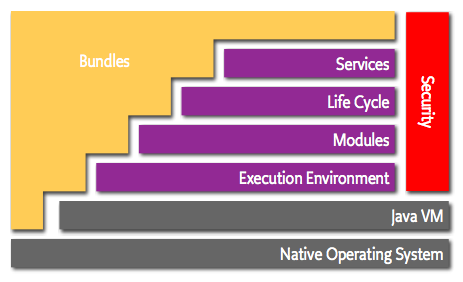
\includegraphics[width=10cm]{grafiken/osgi.png}
	\caption{\acs{osgi} Archetkur~\cite{osgiarch}}
	\label{osgiarch}
\end{figure}

Wie in Abbildung \ref{osgiarch} zu erkennen, ist die \acs{osgi} Service
Plattform als Schichtenarchitektur aufgebaut. Die Architektur setzt sich aus den
folgenden Schichten zusammen~\cite{osgiarch}:

\begin{itemize}
  \item \textbf{\em Bundles:} Bundles stellen die
  Modularisierungseinheit der \acs{osgi} Service Plattform dar. Diese
  k�nnen dynamisch in die Plattform installiert und gestartet, gestoppt und 
  deinstalliert werden, ohne dass die Plattform neu gestartet oder angehalten 
  werden muss. 
  \item \textbf{\em Services:} Die Service-Schicht erlaubt das dynamische
  Verlinken verschiedener Bundles untereinander. Das kann zum Austausch von
  Daten zwischen den Bundles oder zur Ausf�hrung von Funktionalit�ten genutzt werden.
  \item \textbf{\em Life Cycle:} Der Life Cycle k�mmert sich um das Bundle
  Management. Es k�nnen dar�ber Bundles installiert und gestartet, gestoppt und
  deinstalliert werden.
  \item \textbf{\em Modules:} Diese Schicht beschreibt, wie Code von Bundles
  exportiert und von anderen Bundles importiert werden kann. Dabei wird
  sichergestellt, dass nicht exportierter Code, nicht von anderen Bundles
  verwendet werden kann. Neben der Sicherstellung von Import und Export k�mmert
  sich diese Schicht auch um die Versionierung von freigegebenen Schnittstellen.
  So kann dieselbe Schnittstelle in unterschiedlichen Versionen parallel
  verwendet werden.
  \item \textbf{\em Security:} Die Security-Schicht k�mmert sich um das
  Rechtemanagement innerhalb der \acs{osgi} Service Plattform. So lassen sich
  Bundles soweit einschr�nken, dass bestimmte Aktionen erlaubt oder verboten
  sind. Diese Schicht geh�rt nicht zu den Kernkomponenten der
  \acs{osgi}-Plattform und ist somit optional.
  \item \textbf{\em Execution Environment:} Diese Schicht spezifiziert die
  Mindestanforderungen an die Laufzeitumgebung, zur Ausf�hrung der \acs{osgi}
  Service Plattform.
\end{itemize}

\subsection{Verf�gbare \acs{osgi}-Container f�r Android}
Dadurch das Android auf einer Teilmenge des Apache Harmony Projektes basiert,
deckt es einen Gro�teil der Standard Java
Klassenbibliothek~\cite{apacheharmony}. Das erlaubt die Ausf�hrung von
\acs{osgi} auf Android. Die Ausf�hrungsumgebung der Bundles wird auch als
\acs{osgi}-Container bezeichnet. Folgende \acs{osgi} Container sind unter
Android lauff�hig.

\subsubsection{Apache Felix}
Apache Felix ist eine Open-Source-Implementierung des \acs{osgi} R4 Version 4.2
Standards~\cite{apachefelix}. Es ist der zurzeit einzige auf Android lauff�hige
freie \acs{osgi}-Container. Leider bietet Apache Felix keine Integration in das
Android System. Es l�sst sich zurzeit nur per Konsole starten und verwalten.
Das macht es aufwendig Android Anwendungen zu entwickeln, die in Apache Felix
laufen~\cite{apachefelixandroid}.

\subsubsection{Dynamix Framework}
Das Dynamix Framework ist eine Open-Source Middleware um die Entwicklung von
kontextsensitiven Anwendungen f�r Android Smartphones zu vereinfachen. Das
Framework l�uft im Hintergrund auf dem Android Smartphone. Durch die Verwendung
von dynamisch installierten Plug-Ins, die durch die Dynamix Infrastruktur zur
Verf�gung gestellt werden, modelliert das Framework Kontextinformationen.
Kontextinformationen werden durch die Sensorik oder andere externe Systeme
zur Verf�gung gestellt. Die Informationen k�nnen dann anderen auf dem
Smartphone installierten Anwendungen, in einer sicheren Art und Weise zur
Verf�gung gestellt werden.

Das Dynamix Framework basiert auf dem \acs{osgi}-Container Apache Felix.
Plug-Ins werden in Form von Bundles installiert. Das Framework k�mmert
um den Lebenszyklus eines Plug-Ins und erlaubt das Senden von
Kontextinformationen an registrierte Anwendungen. Der vom Dynamix Framework zur
Verf�gung gestellt \acs{osgi}-Container bietet eine Integration in das Android
System. Dynamix l�uft als Service im Hintergrund und erlaubt durch
die sogenannte Context-Firewall, einen kontrollierten Zugriff durch registrierte
Anwendungen, auf die von den Plug-Ins generierten Kontextinformationen. Der
Zugriff kann durch den Anwender geregelt werden~\cite{dynamixframework}.

\section{Datenpersistierung mit db4o}
\acs{db4o} ist eine Objektdatenbank f�r die Java und .NET Plattform, die sich
durch ihre geringe Gr��e von nur 600~KB f�r die Einbettung in Anwendungen
eignet. Durch ihre geringe Gr��e eignet sie sich auch f�r die Verwendung auf mobilen Ger�ten
wie Smartphones, in diesem Fall Android. \acs{db4o} ist eine
Alternative zu der in Android enthaltenden relationalen Datenbank {\em SQLite}.
So ist \acs{db4o} schemafrei und erlaubt die Speicherung beliebig komplexer Objekte,
ohne die Verwendung eines \acfp{orm}. Die Datenspeicherung erfolgt
wie bei {\em SQLite} in einer Datei. \acs{db4o} verwendet im Gegensatz zu
relationalen Datenbanken kein \acs{sql}, sondern \acf{qbe}, Critera Queries
sowie native Anfragen. Bei \acs{qbe} wird anhand eines Beispielobjektes nach
�hnlichen Objekten gesucht. Bei Critera Queries werden \acs{sql} Anfragen durch
eine Verkettung von Methodenaufrufen nachgebildet und bei nativen Queries k�nnen
beliebig komplexe Suchanfragen in Java direkt implementiert werden.

	\chapterfin
	\chapter{Konzeption}
\label{cha:konzeption}
Im Folgenden wird auf die Konzeption der Anwendung eingegangen. Die Konzeption
umfasst die �berf�hrung der Anforderungen in ein Vorgehen, wie die Anforderungen
softwareseitig realisiert werden k�nnen.

\section{Plug-In System}
Ein Erweiterungssystem oder wie hier benannt Plug-in System k�mmert sich um die
Verwaltung von Erweiterungen bzw. Plug-Ins. Das Plug-In System erlaubt die
Erweiterung der Anwendung auch nach ihrer Installation auf dem Smartphone. In
diesem Fall soll die Anwendung im Nachhinein um Plug-Ins erweitert werden, die
Sensordaten sammeln.

Zur Realisierung eines Plug-Ins Systems auf Android gibt er zwei Ans�tze. Der
Erste umfasst die Verwendung eines bereits existierenden Plug-Ins Systems (z.~B.
\acs{osgi}) und der Zweite die Entwicklung eines eigenen Plug-Ins Systems. Im
Folgenden sollen die zwei Ans�tze genauer betrachtet werden.

\subsection{Evaluation der \acs{osgi}-Plattform f�r Android}
Die Verwendung von \acs{osgi} als Modularisierungs- bzw. Plug-In System w�rde
folgende Vorteile bieten:

\begin{itemize}
  \item Modularisierung und dynamisches Laden von neuen Erweiterungen.
  \item Ausf�hrung von Erweiterungen in einer Art Sandbox. Damit ist gemeint,
  dass durch die Bereitstellung separater {\em ClassLoader} der Zugriff auf
  einzelne Elemente der Bibliothek verhindert werden kann.
  \item Versionierung von Plug-Ins.
\end{itemize}

Eine eigenst�ndige Integration von \acs{osgi} in Android war im Rahmen dieser
Masterarbeit aus zeitlichen Gr�nden nicht m�glich. Grund hierf�r ist die
abweichende Entwicklung von Anwendungen f�r Android und Java SE und die daraus
resultierende n�tige Anpassung von \acs{osgi} an Android. Der Aufwand war
zeitlich nur schwer absch�tzbar. Die Verwendung eines bereits f�r Android
optimierten Frameworks ist somit unumg�nglich. Als einziges freies Framework
steht zurzeit nur das Dynamix Framework zur Verf�gung. Eine Verwendung des
Dynamix Frameworks war aber zum Bearbeitungszeitpunkt der Arbeit leider nicht
m�glich. Dem Autor wurde in einem pers�nlichen Gespr�ch mit dem Dynamix
Entwickler Dr.-Ing. Darren Carlson von dessen Verwendung abgeraten. Der Grund
hierf�r war das recht fr�he Stadium des Frameworks und die damit verbundene
m�gliche Fehleranf�lligkeit sowie die fehlende Dokumentation. Die Entwicklung
eines eigenen Plug-Ins Systems war somit die einzige L�sung.

\subsection{Eigenentwicklung eines Plug-In Systems f�r Android}
\label{pluginsystemforandroid}
Bei der Entwicklung eines Plug-In Systems f�r Android gibt es zwei Ans�tze:

\begin{itemize}
  \item Man l�dt zur Laufzeit das Plug-In aus einem nachtr�glich
  heruntergeladenen \acf{jar}. Das w�re der Ansatz von \acs{osgi}.
  \item Man sieht ein Plug-In als Android Service an und kommuniziert mit diesem
  �ber {\em Intents} oder per \acs{ipc}.
\end{itemize}

Ersteres hat den Nachteil, dass eine Infrastruktur geschaffen werden m�sste, um
die Plug-Ins zur Verf�gung zu stellen. Letzteres hat den Vorteil, dass ein
Plug-In als einfache Android Anwendung aus dem Android Market heruntergeladen und
installiert werden kann. Die Infrastruktur ist also schon vorhanden. Auch ist
Letzteres der Ansatz, der vom Android System am besten unterst�tzt wird.

Plug-Ins k�nnen somit als {\em Service} angesehen werden. Nach der Installation
eines Plug-Ins sollen sich neue Plug-Ins beim Plug-In System registrieren. Dazu soll
das Plug-In System, nachdem es �ber die Installation eines neuen Plug-Ins per
{\em Broadcast} benachichtigt wurde, einen {\em Intent} an das neu installierte
Plug-In schicken. Das neue Plug-In soll daraufhin mit entsprechenden
Plug-In Informationen antworten. Folgende Informationen sollen bei der Anmeldung
�bermittelt werden:

\begin{itemize}
  \item Der {\bf Name} des Plug-Ins.
  \item Die {\bf Action}, �ber die der Service per \acs{ipc} aufrufbar ist.
  \item Die {\bf Version} des Plug-Ins.
  \item Die {\bf \acs{url}}, an die die gesammelten Daten �bertragen werden
  sollen.
  \item Die {\bf Periode}, die angibt, in welchen Zeitabst�nden Daten gesammelt
  werden sollen.
  \item Die maximale {\bf Ausf�hrungsdauer} des Plug-Ins, bevor es gestoppt
  wird.
  \item Eine Plug-In {\bf Beschreibung}.
  \item Der {\bf Intervall}, in dem die Daten regelm��ig �bertragen werden
  sollen.
  \item Eine Liste von {\bf Services}, auf die das Plug-In zugreifen will.
  \item Eine Flag die angibt, ob die {\bf gesammelten Daten nach der
  �ber\-tragung gel�scht} werden sollen.
\end{itemize}

Hierbei ist anzumerken, dass Android nicht zwischen einem Plug-In und einer
anderen neu installierten Anwendung unterscheiden kann. Das Plug-In System
sendet somit an alle neu installierten Anwendungen eine Aufforderung zur
Registrierung. Alle Anwendungen die kein Plug-In sind antworten auf die
Anfrage nicht.

Hat sich ein Plug-In erfolgreich registriert, werden die vom Plug-In
erhaltenden Informationen gespeichert und dem Benutzer in Form einer Plug-In
�bersicht pr�sentiert. Der Benutzer hat nun die M�glichkeit sich alle zuvor
beschriebenen Informationen anzuschauen. Dadurch soll der Benutzer die
M�glichkeit erhalten zu entscheiden, ob ein Plug-In wirklich verwendet werden
soll oder nicht.

Ein Plug-In soll bestimmte Zust�nde einnehmen k�nnen. Nach der
Installation soll ein Plug-In als neu dargestellt werden. Das bedeutet der
Benutzer hat das Plug-In bisher nur installiert und noch keine weiteren
Einstellungen am Plug-In vorgenommen. Von diesem Zustand aus soll das Plug-In
aktiviert werden k�nnen. Das hei�t, das Plug-In wird in der bei der
Registrierung angegebenen Periode ausgef�hrt. Soll ein Plug-In keine Daten mehr
sammeln, kann der Benutzer das Plug-In deaktivieren. Sollte ein aktiviertes
Plug-In nach einer bestimmten Zeitspanne genug Daten gesammelt haben, soll es in
den Transferzustand �bergeben. Die Zeitspanne soll bei der Plug-In
Registrierung angegeben werden. In diesem Zustand sollen die Daten f�r die
�bertragung aufbereitet und lokal gespeichert werden. Wann die Daten
endg�ltig �bertragen werden, soll der Benutzer selbst entscheiden. Siehe hierzu
den Abschnitt \ref{periodicallytransfer}. Sind die Daten aufbereitet und
gespeichert worden, geht das Plug-In wieder in den aktivierten Zustand �ber.
Der Lebenszyklus des Plug-Ins ist in Grafik \ref{states} dargestellt.

\begin{figure}[h!] 
	\centering
	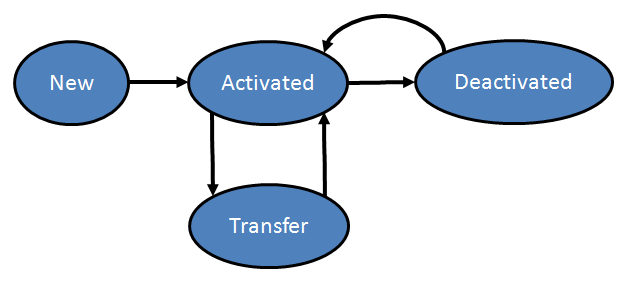
\includegraphics[width=10cm]{grafiken/states.png}
	\caption{Lebenszyklus eines Plug-Ins}
	\label{states}
\end{figure}

M�chte ein Benutzer ein Plug-In wieder entfernen, kann er das �ber den
Anwendungsmanager von Android machen. Der Benutzer soll aber auch direkt die
M�glichkeit besitzen, das Plug-In aus der �bersicht zu entfernen. 

Bei der Deinstallation eines Plug-Ins erh�lt das Plug-In System ebenfalls einen
{\em Broadcast} dar�ber, dass eine Anwendung entfernt wurde. Das erlaubt dem
Plug-In System die gespeicherten Daten vom Plug-In zu l�schen und die Plug-In
Informationen konsistent zu den anderen installierten Plug-Ins zu halten.

\section{Transparentes Sammeln von personenbezogenen Daten}
Transparenz beim Sammeln von personenbezogenen Daten erh�lt man durch folgende
Voraussetzungen:

\begin{itemize}
  \item Der Benutzer muss immer die Kontrolle �ber ein Plug-In besitzen.
  \item Eine Manipulation, bei der Darstellung der personenbezogenen
  Daten, darf nicht m�glich sein.
  \item Alle Daten, die zu einem sp�teren Zeitpunkt �bertragen werden sollen,
  d�rfen nicht im Plug-In selbst gespeichert, sondern m�ssen zentral in
  der Anwendung abgelegt werden.
  \item Bevor die Daten �bertragen werden, muss der Benutzer darauf hingewiesen
  werden, damit eine Kontrolle der Daten vor der �bertragung stattfinden kann.
  \item Der Zugriff auf die Android System Services (die gemeinsamgenutze
  Ressourcen des Systems darstellen und potenziell personenbezogene Daten
  sammeln) wird protokolliert und das Protokoll kann zu jedem Zeitpunkt vom
  Benutzer eingesehen werden.
\end{itemize}

Die Voraussetzungen werden im Folgenden genauer erl�utert.

\subsection{Sichere und kontrollierte Ausf�hrung von Plug-Ins}
\label{securepluginexecution}
Ein Plug-In wird dann sicher ausgef�hrt, wenn der Zugriff auf personenbezogene
Daten bzw. Android System Services kontrolliert stattfindet. Es
sollte also geregelt werden, auf welche Services zugegriffen werden darf und
wenn ein Zugriff stattfindet, sollte der Zugriff protokolliert werden. Des
Weiteren sollte der Zugriff auf bestimmte Daten, die den Benutzer eindeutig
identifizieren (z.~B. \acs{imsi}, Telefonnummer) komplett unterbunden werden.
Aus diesem Grund sollen dem Plug-In nicht die original Android System Services
zur Verf�gung gestellt werden, sondern stattdessen �berwachte bzw. sichere
Implementierungen der Android System Services. Die sicheren Services sollen
jeden Methodenzugriff protokollieren und zuvor beschriebene gef�hrliche Methoden gar
nicht erst anbieten. Folgende Android System Services m�ssen durch sichere
Implementierung ersetzt werden:

\begin{itemize}
  \item {\bf ConnectivityManager}: Erlaubt den Zugriff, auf aktuelle
  Netzwerkinformationen, auf die der Benutzer zugreifen kann.
  \item {\bf LocationManager}: Erlaubt den Zugriff auf, Methoden zur
  Positionsbestimmung des Benutzers.
  \item {\bf TelephonyManager}: Erlaubt den Zugriff auf Telefonfunktionalit�ten.
  \item {\bf WifiManager}: Erlaubt das Auffinden und den Zugriff auf
  \acsp{wlan}.
\end{itemize}

Dabei sollen einem Plug-In nicht von vorne rein alle Services �bergeben werden,
sondern nur die, die in den Plug-In Informationen angegeben wurden. Sollte ein
Plug-In trotzdem versuchen auf einen Android System Services zuzugreifen, soll
das dem Benutzer bei der Aktivierung angezeigt werden. Der unerlaubte Versuch Zugriff
auf einen Android System Service zu erlangen, kann �ber die angeforderten
Rechte des Plug-Ins entnommen werden. Es muss also vor der Aktivierung eine
Kontrolle stattfinden.

Das entwickelte Konzept erweitert die von Android zur Verf�gung
gestellte Sandbox, um weitere �berwachungsmechanismen, um den Schaden, der durch
ein Plug-In entstehen kann zu verringern. Der hierbei gr��te anzunehmende
Schaden ist die �bertragung von personenbezogenen Daten, ohne das Wissen und die
Erlaubnis des Benutzers.

\subsection{Einheitliche Pr�sentation von gesammelten Daten}
\label{unifiedrepresentation}
Um die von einem Plug-In gesammelten Daten einheitlich pr�sentieren zu k�nnen,
muss ein entsprechendes Datenformat gew�hlt werden, an das sich alle Plug-Ins halten
m�ssen. Da die Struktur der Daten nicht bekannt ist, muss ein Datenformat
verwendet werden, dass unstrukturierte Daten abbilden kann. Ein solches
Datenformat wird in dem \acf{jsr} 170 beschrieben~\cite{jsr170}. Der
\acs{jsr} beschreibt die Speicherung von Daten im \acf{jcr}. Das im
\acs{jsr}-170 beschriebene Datenformat basiert auf Knoten ({\em Nodes}) und
Eigenschaften ({\em Properties}), die sich zu einer beliebigen hierarchischen
Datenstruktur zusammensetzen lassen. Im Rahmen dieser Masterarbeit soll eine eingeschr�nkte
Implementierung des Standards stattfinden, die Funktionalit�ten wie z.~B.
Versionierung und Locking nicht ber�cksichtigt. Diese sind f�r die Erf�llung der
Aufgabenstellung nicht notwendig.

\begin{figure}[h!] 
	\centering
	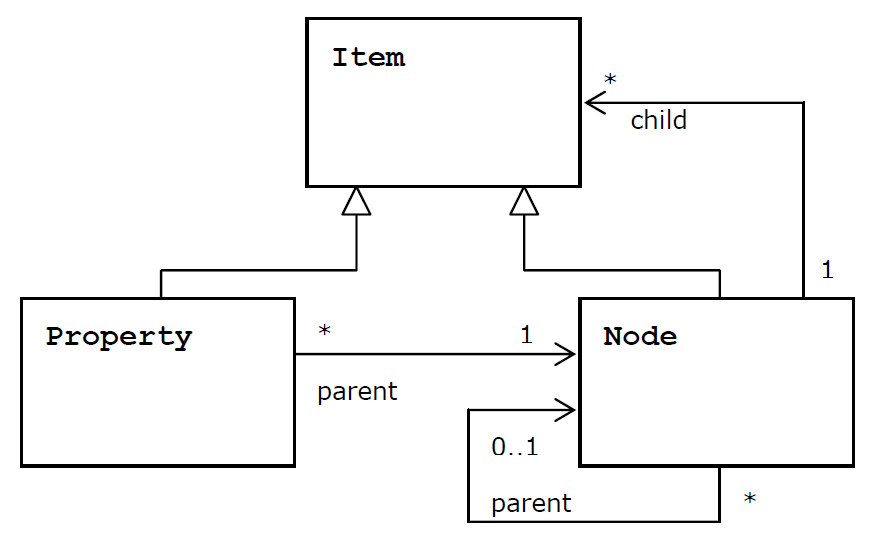
\includegraphics[width=12cm]{grafiken/jsr170.png}
	\caption{UML-Diagramm f�r \acs{jsr}-170\cite[Seite 22]{jsr170}}
	\label{jsr170}
\end{figure}

Abbildung \ref{jsr170} zeigt in einem UML-Diagramm die Zusammenh�nge zwischen
den einzelnen Klassen. Wie zu erkennen gibt es eine gemeinsam genutzte Klasse
mit dem Namen {\em Item}. Die Klasse enth�lt eine Obermenge von Attributen die
Knoten und Eigenschaften besitzen. Die Attribute sind eine eindeutige ID,
ein Modifizierungsdatum sowie der Elternknoten. Ein Knoten kann beliebige viele
Kinderknoten und Eigenschaften besitzen. Eine Eigenschaft besteht aus
einem Namen und einem Wert. Der Wert selbst besteht aus dem eigentlichen
zu speichernden Wert sowie dem Typen des Wertes. Ein Wert kann vom Typ
{\em String}, {\em Date}, {\em Binary}, {\em Double}, {\em Decimal}, {\em Long}
oder {\em Boolean} sein.

Zur Pr�sentation soll ein Betrachter entwickelt werden, der die hierarchischen
Daten darstellen kann. Dabei soll jede Hierarchiestufe in Form einer Liste
angezeigt werden. Innerhalb der Liste werden alle Knoten und Eigenschaften
aufgef�hrt. W�hlt man  einen Knoten aus, so soll man in die n�chste
Hierarchiestufe gelangen. �ber die Zur�cktaste soll man wieder eine
Hierarchiestufe zur�ck gelangen. Als Darstellungswert innerhalb der Liste soll
bei einem Knoten das Modifizierungsdatum und bei einer Eigenschaft eine
Kombination aus dem Namen und der String-Repr�sentation des Wertes verwendet
werden.

\subsection{Speicherung der Daten}
Die Speicherung der Daten soll zentral in der Anwendung geschehen und in
dem, in Abschnitt \ref{unifiedrepresentation}, beschriebenen Datenformat erfolgen. Durch die
zentrale und unmittelbare Speicherung der Daten als vereinheitlichte
Datenstruktur kann eine sofortige Pr�sentation der Daten geschehen, ohne die
Daten beim Plug-In selbst nachzufragen zu m�ssen. So m�ssen keine Daten vom
Plug-In selbst gespeichert werden, die Persistierung wird von der Anwendung
�bernommen. Die Speicherung der Daten soll per \acs{db4o} erfolgen. \acs{db4o}
erlaubt die einfache Speicherung von komplexen hierarchischen Datenstrukturen, wie sie
im Abschnitt \ref{unifiedrepresentation} beschrieben ist.

Bei der Ausf�hrung eines Plug-Ins soll dieses vollen Zugriff, auf die
zuvor gespeicherten Daten, besitzen. Dadurch soll die M�glichkeit bestehen zuvor
gespeicherte Daten nachtr�glich zu bearbeiten und neue Datens�tze hinzuzuf�gen.

\subsection{Regelm��ige �bertragung der gesammelten Daten}
\label{periodicallytransfer}
Im Gegensatz zu anderen Anwendungen, in dem die Daten sofort ohne R�ckfrage des
Benutzers �bertragen werden, sollen sie in dieser Anwendung nur in regelm��igen
Abst�nden und nur nach Erlaubnis des Benutzers �bertragen werden. Die Abst�nde
sollen durch das Plug-In selbst definiert werden. Wird als �bertragungsintervall
z.~B. ein Tag angegeben, so soll der Benutzer, wenn das Plug-In ein Tag lang
aktiv war, in den zuvor beschriebenen Transferzustand �bergehen. Sollte das
Plug-In in dieser Zeit deaktiviert worden sein, soll diese Zeit nicht in die
�bertragungszeit mit eingerechnet werden. Es wird nur die Zeit beachtet, in der
das Plug-In aktiv war.

Befindet sich das Plug-In im Transferzustand, sollen die bis zu diesem Zeitpunkt
vom Plug-In gesammelten Daten gesichert und f�r die �bertragung vorbereitet werden. Das
Plug-In kann nun wieder aktiviert werden und weiter Daten sammeln. Der Benutzer
soll vor der �bertragung alle angefallenden Daten des Plug-Ins einsehen
k�nnen, das hei�t, alle Zugriffe auf die Services sowie die vom Plug-In
gesammelten Daten.

Ist der Benutzer mit einer �bertragung der Daten einverstanden, kann er die
Daten zu einem beliebigen Zeitpunkt in der Zukunft �bertragen. Die Daten sollen
daraufhin an die, in den Plug-In Information enthaltenen \acs{url} �bertragen
werden. Sollte der Benutzer nicht mit der �bertragung der Daten einverstanden sein, so
soll er die M�glichkeit besitzen, die vom Plug-In gesammelten Daten zu
verwerfen. Da eine �bertragung zu einem beliebigen Zeitpunkt in der Zukunft
stattfinden kann, kann es passieren, dass sich mehrere �bertragungen ansammeln
k�nnen. Alle �bertragungen sollen �bersichtlich aufgelistet werden.

Bei der �bertragung m�ssen neben den gesammelten Daten, auch
Informationen �ber das verwendete Plug-In und eine eindeutige Benutzerkennung
versendet werden. Dadurch kann auf der Serverseite eine eindeutige Zuordnung
zu einem Plug-In sowie zu einem Benutzer stattfinden. Die
verwendete Benutzerkennung muss anonymisiert sein (siehe Abschnitt
\ref{anonymisation}).

\section{Serverseitiger Empfang und Verarbeitung der Daten}
Neben der reinen Android Anwendung soll auch eine Serverkomponente ent\-wickelt
werden, die die vom Plug-In gesammelten Daten empfangen kann. Zum Empfang der
Daten auf dem Server sollen bereits bekannte Standards wie das \acf{http}, der
\acf{rest} und die \acf{json} verwendet werden. \acs{rest} erlaubt den Zugriff
und die Manipulation von entfernten Objekten per \acs{http}. Dazu soll auf dem
Server ein \acs{rest}ful Webservice zur Verf�gung gestellt werden, um die von
der Anwendung in \acs{json} codierten Daten zu empfangen. \acs{json} erlaubt die
Codierung von Daten in einem Menschen lesbarem Format, besitzt einen
geringen Overhead, im Vergleich zu \acs{xml} und ist ein mittlerweile
anerkannter Standard zur �bertragung von Daten �bers Internet~\cite{json}.

Da die Daten von der Anwendung in dem zuvor beschriebenen sehr allgemeinen
Datenformat empfangen werden, ist eine Konvertierung der Daten in ein
spezifischeres Datenformat vorzunehmen. Die Konvertierung sollte in ein
dom�nen\-spezi\-fisches Datenformat stattfinden und muss vom Plug-In Entwickler
selbst vorgenommen werden. Das ist aus den folgenden Gr�nden zu empfehlen:

\begin{itemize}
  \item Die Verwaltung des allgemeinen Datenformats ist innerhalb von nicht
  objektorientierten Datenbanken sehr aufwendig. Das wird vor allen dingen dann
  sichtbar, wenn man versucht die Datenstruktur in relationalen Datenbanken zu
  speichern.
  \item Ein dom�nenspezifisches Datenformat erlaubt die einfachere Verarbeitung
  der Daten gegen�ber dem allgemeinen Datenformat. Auch wird die Flexibilit�t
  des allgemeinen Datenformats in weiteren Verarbeitungsschritten nicht mehr
  ben�tigt. Die Komplexit�t der Anwendung kann dadurch reduziert werden.
\end{itemize}

\section{Anonymisierung des Benutzers}
\label{anonymisation}
Wie bereits in Abschnitt \ref{anonym} beschrieben, k�nnen die von der Anwendung
empfangenen Daten ohne eine eindeutige Benutzerkennung nicht �ber mehrere
�bertragungen zu einem Benutzer zugeordnet werden. Die Zuordnung ist aber
notwendig, wenn man z.~B. die Bewegungen von Personen �ber einen l�ngeren
Zeitraum �berwachen m�chte. Ohne eine Benutzerkennung w�re dies immer nur
innerhalb eines �bertragenden Datensatzes m�glich. Um das Problem zu
l�sen, ist eine eindeutige Benutzerkennung n�tig, die bei jeder �bertragung mit
gesendet wird. Bei der Benutzerkennung ist auf Folgendes zu achten:

\begin{itemize}
  \item Durch die Benutzerkennung darf man auf keine reale Person schlie�en
  k�nnen.
  \item Die Benutzerkennung muss zwischen verschiedenen Plug-Ins unterschiedlich
  sein.
  \item Auch bei einem Wechsel des Ger�ts soll dieselbe eindeutige
  Benutzerkennung ohne jegliche Interaktion mit dem Benutzer generiert werden
  k�nnen.
\end{itemize}

Um eine eindeutige Benutzerkennung zu berechnen, m�ssen eindeutige Werte vom
Plug-In, sowie vom Benutzer verwendet werden. Da der Wert vom Benutzer ohne
Interaktion ermittelt werden soll, muss hier ein Wert verwendet werden, der
Benutzer spezifisch ist und sich bereits auf dem Smartphone befindet. Zu diesem
Zweck kann die \acs{imsi} verwendet werden. Die Nummer identifiziert einen
Benutzer eindeutig im \acs{gsm}- und \acs{umts}-Netz. Als Plug-In Wert kann die
{\em Action} verwendet werden, die f�r jedes Plug-In eindeutig ist.

Aus der Kombination von Plug-In spezifischer {\em Action} und \acs{imsi} l�sst
sich nun eine eindeutige Benutzerkennung berechnen. Zur Berechnung eignen sich
Hashfunktionen. Diese erlauben die Generierung von eindeutigen Werten und sind
nur mit sehr hohem Aufwand umkehrbar. Als Hashfunktion soll eine aus der Gruppe der
\acs{sha}-2 Algorithmen verwendet werden, da jene das zurzeit sicherste
Verfahren verwenden. Die eindeutige Benutzerkennung kann nun durch die
Konkatenation aus Plug-In Action und \acs{imsi} und der anschlie�enden Anwendung eines
\acs{sha}-2 Algorithmus berechnet werden. Die sich dadurch ergebene
Benutzerkennung bietet maximale Anonymit�t bei maximalem Komfort des Benutzers.
Die Kennung soll nun bei jeder �bertragung mit �bertragen werden.

	\chapterfin
	\chapter{Realisierung}
\label{cha:realisierung}
In diesem Kapitel wird die aus dem Konzept entwickelte Realisierung beschrieben.
Die Anwendung tr�gt den Arbeitstitel {\em Mobile Data Collector},
w�h\-rend das Framework zur Erstellung von Plug-Ins den Namen {\em Mobile Data
Collection Framework} tr�gt.

Der {\em Mobile Data Collector} wird als Open Source Projekt entwickelt und kann
entweder von der beiliegenden CD oder von GitHub unter der Adresse
\url{https://github.com/mlegenhausen/mdcf} bezogen werden. Das Projekt ist
in die folgenden Teile gegliedert:

\begin{itemize}
  \item {\bf MobileDataCollector}: Die {\em Mobile Data Collector}
  Android-Anwendung, die die komplette Anwendungslogik zur Ausf�hrung von
  Erweiterungen enth�lt.
  \item {\bf MobileDataCollectionFramework}: Das Framework zur Entwicklung von
  Erweiterungen (Plug-Ins).
  \item {\bf LocationTrackerPlugin}: Ein Beispiel-Plug-In zum Sammeln von
  Standortdaten.
  \item {\bf NoiseTrackerPlugin}: Eine Erweiterung des {\em
  LocationTrackerPlugin}, bei dem neben der aktuellen Position, auch die
  Lautst�rke gespeichert wird.
  \item {\bf mdcf-remote}: Das Framework zur Entwicklung der Serverkomponente.
  \item {\bf mdcf-locationtracker-remote}: Eine Beispielserverkomponente f�r
  das {\em LocationTrackerPlugin}.
  \item {\bf mdcf-noisetracker-remote}: Eine Beispielserverkomponente f�r das
  {\em NoiseTrackerPlugin}.
\end{itemize}

\section{Architektur des Mobile Data Collection Frameworks}
Das {\em Mobile Data Collection Framework} dient zur Erstellung von Plug-Ins. Es
beinhaltet alle Klassen und Schnittstellen, die zwischen dem {\em Mobile Data
Collector} und dem Plug-In geteilt werden, um eine Kommunikation zwischen beiden
Komponenten zu erm�glichen. Das Framework wird als Android-Bibliothek zur
Verf�gung gestellt.

Das Framework ist in drei Teile gegliedert. Zum einen Klassen und Interfaces,
die es einem Plug-In erlauben, sich an dem Plug-In-System anzumelden und mit
diesem zu kommunizieren. Zum anderen einer Implementierung der in Abschnitt
\ref{unifiedrepresentation} beschriebenen Datenstruktur sowie der in Abschnitt
\ref{securepluginexecution} beschriebenen sicheren {\em Android System Services}.

Ein Plug-In wird dadurch definiert, dass es die {\em Plugin}-Schnittstelle
implementiert. Diese stellt alle f�r das Plug-In-System n�tigen Methoden
zur Verf�gung, um mit dem Plug-In zu interagieren. Die Schnittstelle selbst
besteht aus einer Reihe von {\em Settern}, mit denen die sicheren Versionen der
{\em Android System Services} und der {\em PersistenceManager} gesetzt werden, sowie
einer {\em run}-Methode, mit der das Plug-In ausgef�hrt wird. Auf Folgende
sichere Versionen der {\em Android System Services} kann ein Plug-In zugreifen:

\begin{itemize}
  \item {\bf ConnectivityManager}: Erlaubt den Zugriff, auf aktuelle
  Netzwerkinformationen.
  \item {\bf LocationManager}: Erlaubt den Zugriff auf, Methoden zur
  Positionsbestimmung des Benutzers.
  \item {\bf TelephonyManager}: Erlaubt den Zugriff auf Telefonfunktionalit�ten.
  \item {\bf WifiManager}: Erlaubt das Auffinden und den Zugriff auf
  \acsp{wlan}.
\end{itemize}

Da die {\em Setter}-Implementierungen trivial und in den meisten F�llen
identisch sind, gibt es zur Vereinfachung die Klasse {\em AbstractPlugin}. Erbt
man von der Klasse, muss nur noch eine vereinfachte Version der {\em
run}-Methode, die {\em onRun}-Methode, implementiert werden.

Innerhalb der {\em run}- bzw. {\em onRun}-Methode kann auf die gesetzten
{\em Android System Services} zugegriffen werden, welche weitestgehend alle in
der Android Dokumentation beschriebenen Methoden bieten. Neben diesen kann
auch auf einen {\em PersistenceManager} zugegriffen werden. Dieser erlaubt �ber die {\em
getWorkspace}-Methode den einfachen Zugriff auf alle bisher gespeicherten Daten.
Die zur�ck\-gegebene Datenstruktur kann dann innerhalb des Plug-Ins beliebig
manipuliert werden. Wurden alle Daten erfolgreich manipuliert, k�nnen die
�nderungen mit der {\em save}-Methode gespeichert werden.

Die Registrierung eines Plug-Ins erfolgt durch die Antwort auf den vom
Plug-In-System versendeten {\em Broadcast}, der nach der Installation einer
neuen Anwendung versendet wird. Um auf den {\em Broadcast} zu antworten, muss
ein {\em Broadcast Receiver} implementiert werden. Zu diesem Zweck existiert
bereits eine Implementierung des {\em Broadcast Receiver}, der {\em
AbstractPluginRegister}. Erbt man von der Klasse, muss man die {\em
onRegister}-Methode implementieren. Diese muss ein {\em PluginInfo}-Objekt
zur�ckliefern, welche die Plug-In-Informationen enth�lt. Bei dem {\em
PluginInfo}-Objekt handelt es sich um ein Java-\acs{pojo}, dass die in Abschnitt
\ref{pluginsystemforandroid} beschriebenen Attribute besitzt. Neben der reinen
Java-Konfiguration kann man das Objekt auch aus einer \acs{xml}-Datei generieren
lassen. Dazu muss man von der {\em XMLPluginRegister}-Klasse erben und den Pfad
zur Konfigurationsdatei als Konstruktorparameter �bergeben. Hierbei muss darauf
geachtet werden, dass die Datei sich im {\em Java Classpath} befindet.

Damit das implementierte Plug-In und der {\em Broadcast Receiver} vom Android
System gefunden werden k�nnen, m�ssen entsprechende Eintr�ge in der {\em
AndroidManifest.xml} erfolgen.

Konkrete Beispiele zur Implementierung und Konfiguration sind dem Kapitel
\ref{cha:leitfaden} zu entnehmen.

\section{Architektur des Mobile Data Collectors}
Die Architektur des {\em Mobile Data Collector} ist in Abbildung
\ref{architecture} dargestellt. Wie in der Abbildung zu erkennen, stellt der
{\em Plug-In Service} (blau) die zentrale Komponente des {\em Mobile Data
Collector} dar. Er beherbergt das gesamte Plug-In-System und k�mmert sich somit
um die Verwaltung und Ausf�hrung von Plug-Ins. Er speichert alle von den
Plug-Ins gesammelten Daten in einer \acs{db4o}-Datenbank (gelb). Sollte ein
Plug-In auf die {\em Android System Services} (grau) zugreifen, geschieht das aus
Transparenzgr�nden ebenfalls �ber den {\em Plug-In Service}.

\begin{figure}[h!] 
	\centering
	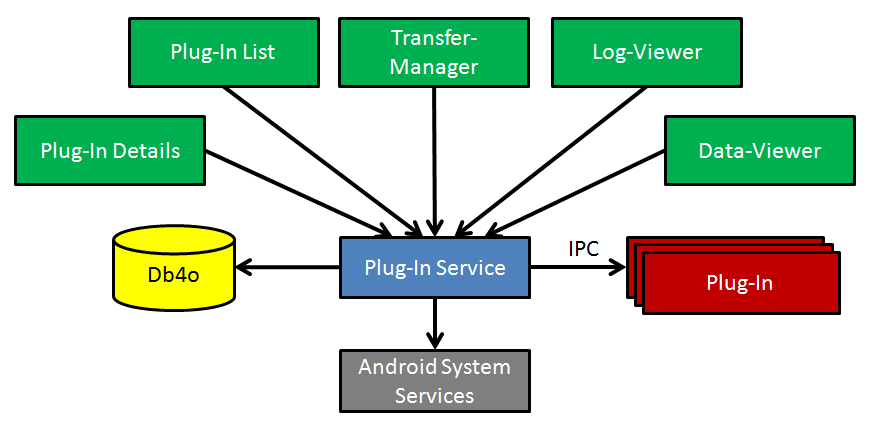
\includegraphics[width=13cm]{grafiken/architecture.png}
	\caption{Architektur des Mobile Data Collector}
	\label{architecture}
\end{figure}

F�r die Benutzerinteraktion mit dem {\em Plug-In Service} stehen eine
F�lle von {\em Activities} (gr�n) zur Verf�gung. Die {\em Activities} sind:

\begin{itemize}
  \item Der {\bf Plug-In List} dient zur Auflistung von installierten Plug-Ins.
  \item Die {\bf Plug-In Details} erlauben die Einsicht von Plug-In-Informationen.
  \item Der {\bf Log-Viewer} dient zur Auflistung aller protokollierten Zugriffe
  auf die sicheren {\em Android System Services} vom {\em Mobile Data Collector}.
  \item Der {\bf Data-Viewer} erlaubt die Betrachtung von allen vom Plug-In
  gesammelten Daten.
  \item Der {\bf Transfer-Manager} listet alle ausstehenden �bertragungen auf
  und erlaubt die nachtr�gliche Betrachtung aller bis zur �bertragung
  gesammelten Daten sowie deren Verwaltung.
\end{itemize}

Die Pfeile ausgehend vom und zum {\em Plug-In Service} stellen die
Aufrufrichtung dar. So ruft z.~B. der {\em Plug-In Service} immer die Plug-Ins
auf, und die {\em Activities} den {\em Plug-In Service}.

Im Folgenden wird auf die zuvor beschriebenen Komponenten genauer eingegangen.

\subsection{Plug-In Service}
Der {\em Plug-In Service} stellt die zentrale Komponente zur Verwaltung von Plug-Ins
sowie deren Ausf�hrung dar. Er beinhaltet die gesamte Applikationslogik des
{\em Mobile Data Collectors}. Alle {\em Activities} greifen �ber eine
entsprechende Schnittstelle auf den {\em Plug-In Service} zu, welcher dauerhaft im
Hintergrund l�uft und die Plug-Ins in den vorgegebenen Zeitabst�nden ausf�hrt.

Neben der Service-Schnittstelle stellt das {\em PluginConfiguration}-Ob\-jekt
eine wichtige Datenstruktur dar. Alle zus�tzlichen Informationen �ber ein Plug-In,
die zur internen Verwaltung ben�tigt werden, werden im {\em
PluginConfiguration}-Ob\-jekt gespeichert. Dieses besitzt folgende Attribute:

\begin{itemize}
  \item {\bf Mode} gibt an, ob sich das Plug-In im {\em New}-, {\em
  Activated}-, {\em Deactivated}- oder {\em Transfer}-Zustand befindet. Im
  Letzteren werden die bisher gesammelten Daten f�r eine �bertragung vorbereitet.
  \item {\bf State} gibt an, ob das Plug-In sich im {\em Resolved}-, {\em
  Waiting}- oder {\em Running}-Zustand befindet. Im {\em Resolved} Zustand
  befindet es sich immer dann, wenn der {\em Mode} {\em New}, {\em Deactivated}
  oder {\em Transfer} ist. Zwischen den Zust�nden {\em Waiting} und {\em Running}
  wechselt das Plug-In, wenn es sich im {\em Mode} {\em Activated} befindet.
  \item {\bf Last Executed} gibt an, wann das Plug-In das letzte Mal ausgef�hrt
  wurde.
  \item {\bf Last Activated} gibt an, wann das Plug-In das letzte Mal aktiviert
  wurde.
  \item {\bf Total Activation Time} gibt summiert an, wie lange das Plug-In
  aktiviert war.
  \item {\bf Permissions} gibt an, welche Zugriffsrechte das Plug-In vom
  Android-Betriebssystem ben�tigt. Im besten Fall ist das Attribut leer, da
  das bedeutet, dass das Plug-In nicht auf reglementierte Ressourcen zugreifen
  muss, sondern alle Aufgaben kontrolliert �ber den {\em Mobile Data Collector}
  ausf�hren kann.
  \item {\bf Log Records} protokolliert alle Zugriffe, die auf den sicheren
  Versionen der {\em Android System Services} stattgefunden haben.
  \item {\bf Transfers} beinhaltet eine Liste von ausstehenden �bertragungen.
  \item {\bf Workspace} beinhaltet alle vom Plug-In gesammelten Daten. Dabei
  handelt es sich um ein {\em Node}-Objekt, an dem alle zus�tzlichen Daten
  angehangt werden k�nnen.
\end{itemize}

Da die {\em PluginConfiguration} alle relevanten Plug-In-Informationen, {\em
Log Records} und alle gesammelten Daten enth�lt, wird die Datenstruktur 
innerhalb der {\em db4o}-Datenbank zur Persistierung verwendet.

\subsubsection{Service-Interface Definition}
Das Service-Interface beinhaltet die folgenden zentralen Methoden:

\begin{lstlisting}[language=java]
void addListener(PluginListener listener)
\end{lstlisting}

Erlaubt das Hinzuf�gen von {\em PluginListener}, die aufgerufen werden, wenn ein
neues Plug-In installiert bzw. entfernt wurde oder das Plug-In seinen {\em
Mode} oder {\em State} ge�ndert hat.

\begin{lstlisting}[language=java]
void addListener(TransferListener listener)
\end{lstlisting}

Erlaubt das Hinzuf�gen von {\em TransferListener}, die aufgerufen werden, wenn
eine neue �bertragung erstellt bzw. entfernt wurde.

\begin{lstlisting}[language=java]
void activate(PluginConfiguration configuration)
\end{lstlisting}

Aktiviert das mit der �bergebenen {\em PluginConfiguration} assoziierte
Plug-In.

\begin{lstlisting}[language=java]
void deactivate(PluginConfiguration configuration)
\end{lstlisting}

Deaktiviert das mit der �bergebenen {\em PluginConfiguration} assoziierte
Plug-In.

\begin{lstlisting}[language=java]
PluginConfiguration getPluginConfiguration(PluginInfo info)
\end{lstlisting}

Liefert die zur {\em PluginInfo} dazu geh�rige {\em PluginConfiguration} zur�ck.
Existiert keine dazugeh�rige {\em PluginConfiguration}, so wird {\em null}
zur�ckgegeben.

\begin{lstlisting}[language=java]
List<PluginConfiguration> getPluginConfigurations()
\end{lstlisting}

Liefert alle installierten Plug-Ins in Form von {\em
PluginConfiguration}-Objekten zur�ck.

\begin{lstlisting}[language=java]
List<Transfer> getTransfers()
\end{lstlisting}

Liefert alle noch ausstehenden �bertragungen zur�ck. Sollten keine
�ber\-tra\-gungen vorhanden sein, wird eine leere Liste zur�ckgegeben.

\begin{lstlisting}[language=java]
void removeTransfer(Transfer transfer)
\end{lstlisting}

Entfernt den �bergebenen Transfer. Diese Methode sollte normalerweise nur dann
aufgerufen werden, wenn das {\em Transfer}-Objekt auch an einen externen Server
�bertragen wurde.

\subsubsection{Plug-In-Registrierung}
Der Vorgang der Plug-In-Registrierung ist in Abbildung \ref{register}
dargestellt.

\begin{figure}[h!] 
	\centering
	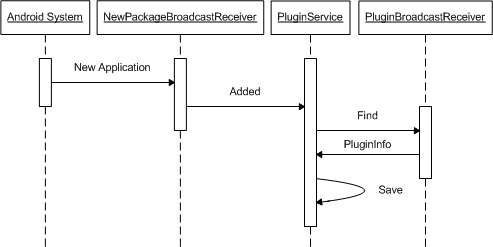
\includegraphics[width=13cm]{grafiken/register.png}
	\caption{Plug-In Registierung}
	\label{register}
\end{figure}

Wie in dem Sequenzdiagramm zu erkennen, sendet als Erstes das Android-System
einen {\em Broadcast} mit dem Inhalt, dass eine neue Anwendung installiert
wurde. Dieser wird vom {\em PackageAddedBroadcastReceiver} empfangen. Daraufhin
versendet jener ein {\em Added-Intent} an den {\em Plug-In Service}, dass eine neue
Anwendung installiert wurde. Der {\em Intent} wird von der {\em
onStartCommand}-Methode des {\em Plug-In Services} empfangen, welcher daraufhin
ein {\em Find-Intent} an die neu installierte Anwendung versendet. Antwortet die
Anwendung nicht, so handelt es sich nicht um ein Plug-In. Antwortet die neu
installierte Anwendung mit einem {\em PluginInfo}-Objekt, so handelt es sich um
ein neues Plug-In.  Das vom Plug-In-System empfangene {\em PluginInfo}-Objekt
wird nun vom {\em Plug-In Service} in einem {\em PluginConfiguration}-Objekt
gespeichert. Das Plug-In gilt somit als registriert. Die weitere Verwaltung des
Plug-Ins findet �ber das {\em PluginConfiguration}-Objekt statt.

\subsubsection{Plug-In Ausf�hrung}
Die Ausf�hrung des Plug-Ins findet im {\em PluginTaskManager} statt. Die
Klasse verwaltet alle aktivierten Plug-Ins und f�hrt diese in dem vom Plug-In
vorgegeben Abstand aus. Dazu verwendet der {\em PluginTaskManager} einen
Thread-Pool, mit dem er eine bestimmte Anzahl von Plug-Ins parallel ausf�hren
kann. Zurzeit besitzt der Thread-Pool eine statische Gr��e von 1. Als
Thread-Pool-Implementierung wurde der {\em ScheduledExecutorService} von der
{\em Java Concurrency} Bibliothek verwendet.

Wurde ein Plug-In aktiviert, wird dessen {\em PluginConfiguration}-Objekt an den
{\em PluginTaskManager} �bergeben. Dieser kapselt das {\em
PluginConfiguration}-Objekt zu einem {\em PluginTask}-Objekt. Beim {\em
PluginTask} handelt es sich um ein aus\-f�hr\-bares Objekt, dass das {\em
Runnable}-Interface implementiert. Der Task wird nun an den zuvor erw�hnten
Thread-Pool zur sofortigen Ausf�hrung �bergeben. Bei der Ausf�hrung wird aus der
{\em PluginInfo} die {\em Action} ausgelesen. Mit dieser ist es m�glich, die
Service-Schnittstelle des Plug-Ins aufzurufen. Konnte eine Verbindung zum
Plug-In hergestellt werden, werden zuerst die in den Plug-In-Informationen
angegebenen sicheren {\em Android System Services} sowie der {\em PersistenceManager}
gesetzt, um daraufhin das Plug-In auszuf�hren. Das Plug-In wird dabei nur
maximal f�r die im {\em PluginInfo} angegebene Zeit ausgef�hrt. Sollte die
Zeit �berschritten werden, so wird das Plug-In vom Android-System terminiert.
Nach der Ausf�hrung wird das Plug-In wieder zum Thread-Pool hinzugef�gt, um ihn
diesmal erst nach dem vom Plug-In definierten Abstand auszuf�hren. Dieser Ablauf
wiederholt sich solange, bis das Plug-In deaktiviert wurde oder eine �bertragung
vorbereitet wird. Da das Plug-In immer im Nachhinein wieder zum
Thread-Pool hinzugef�gt und nicht automatisch periodisch ausgef�hrt wird, wird
eine �berlappung der Plug-In-Ausf�hrungen verhindert.

�ber den {\em PersistenceManager} k�nnen w�hrend der Ausf�hrung beliebige
Informationen innerhalb der Datenbank des {\em Mobile Data Collectors}
gespeichert werden.

Sollte w�hrend der Ausf�hrung ein Plug-In auf Methoden der sicheren {\em Android
System Services} zugreifen, so wird der Zugriff protokolliert. Dazu wird vor
jeder Ausf�hrung ein neuer Eintrag zu den {\em Log Records} der {\em
PluginConfiguration} hinzugef�gt. In einen solchen {\em Log Record} k�nnen nun
beliebig viele Eintr�ge hinzugef�gt werden, die den Zugriff in
menschenverst�ndlicher Sprache protokollieren. Die Eintr�ge lassen sich dann
�ber den in Abschnitt \ref{plugin_details} beschriebenen {\em Log-Viewer}
einsehen.

\subsection{Plug-In List}
Die {\em Plug-In List} dient zur Auflistung aller installierten Plug-Ins. Sind
keine Plug-Ins installiert, wird, wie in Abbildung \ref{pluginlist} zu sehen,
der Benutzer darauf hingewiesen.

\begin{figure}[h!] \centering
	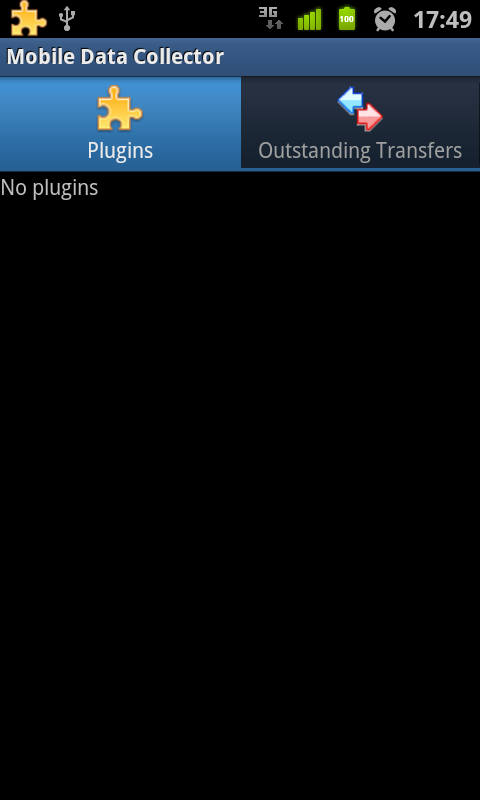
\includegraphics[width=5cm]{grafiken/pluginlist.png}
	\caption{Plug-In Viewer}
	\label{pluginlist}
\end{figure}

Neue Plug-Ins k�nnen �ber Eclipse, dem {\em Android Market} oder von der SD-Card
installiert werden. Um den {\em Android Market} schneller zu erreichen, kann auf
den Market wie in Abbildung \ref{more_plugins} �ber die Men�taste direkt
zugegriffen werden.

\begin{figure}[h!] \centering
	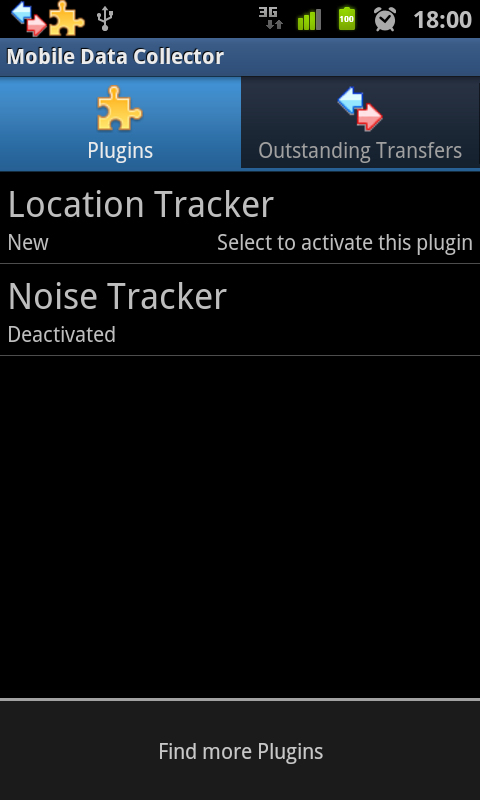
\includegraphics[width=5cm]{grafiken/more_plugins.png}
	\caption{Neue Plug-Ins installieren}
	\label{more_plugins}
\end{figure}

Wurden neue Plug-Ins installiert, werden diese, wie in Abbildung \ref{plugins}
dargestellt, in der {\em Plug-In List} angezeigt. Die installierten Plug-Ins
befinden sich zurzeit im Zustand {\em New}.

\begin{figure}[h!] \centering
	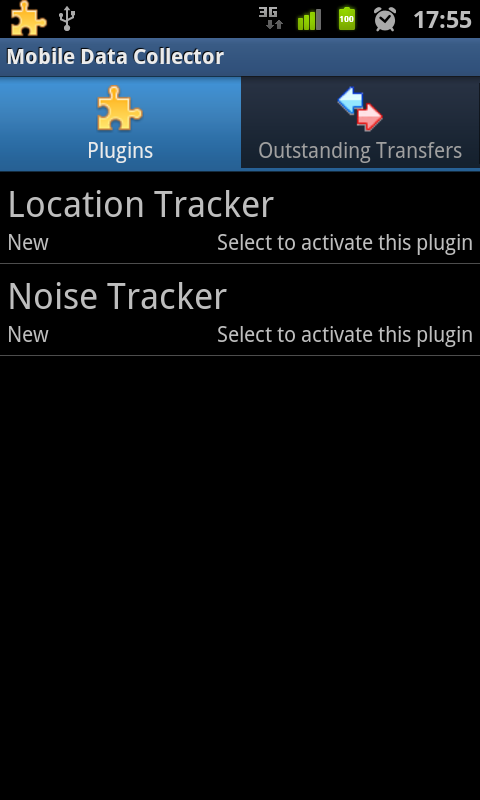
\includegraphics[width=5cm]{grafiken/plugins.png}
	\caption{Installierte Plug-Ins}
	\label{plugins}
\end{figure}

Durch das Anw�hlen eines Plug-Ins kann man dieses aktivieren. Bevor das Plug-In
aktiviert wird, werden, wie in Abbildung \ref{activation} zu sehen, die
Plug-In-Informationen angezeigt. Hat man alle Informationen kontrolliert und ist
mit diesen einverstanden, kann man durch das Dr�cken der {\em Activate}
Schaltfl�che das Plug-In aktivieren. Durch das Dr�cken von {\em Cancel} kann man
den Aktivierungsprozess abbrechen.

\begin{figure}[h!] 
	\centering
	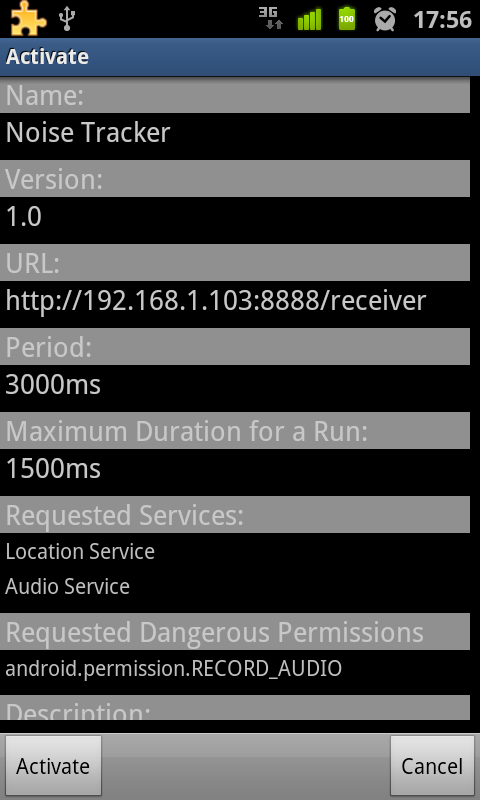
\includegraphics[width=5cm]{grafiken/activation.png}
	\caption{Plug-In-Aktivierung}
	\label{activation}
\end{figure}

Hierbei ist besonders auf die sogenannten {\em Dangerous Permissions} zu achten.
Diese weisen den Benutzer darauf hin, dass das Plug-In Rechte anfordert, �ber
die es auf potenziell personenbezogene Daten zugreifen k�nnte. Vor der
Aktivierung wird deswegen der Benutzer durch die in Abbildung
\ref{activation_warning} dargestellte Warnung dar�ber informiert, um
gegebenenfalls der Aktivierung zu widersprechen.

\begin{figure}[h!] 
	\centering
	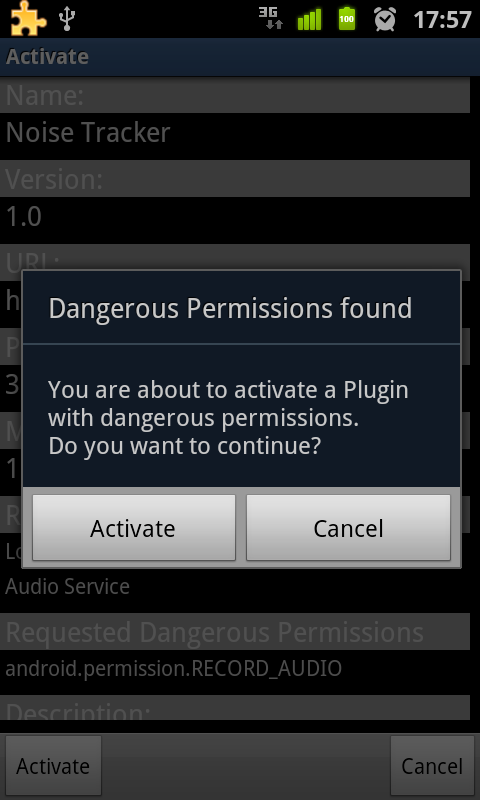
\includegraphics[width=5cm]{grafiken/activation_warning.png}
	\caption{Warnung bei Plug-In-Aktivierung}
	\label{activation_warning}
\end{figure}

Ist sich der Benutzer trotzdem dar�ber bewusst, dass das Plug-In m�glicherweise
gef�hrlich sein k�nnte, so kann er durch das Dr�cken der {\em OK}-Schaltfl�che
das Plug-In trotzdem aktivieren. Durch die {\em Cancel}-Schaltfl�che kann die
Aktivierung abgebrochen werden.

Nach der Aktivierung eines Plug-Ins, wechselt die Anzeige von {\em
New} zu {\em Activated}. Siehe Abbildung \ref{activate}, indem das
{\em Noise Tracker} Plug-In aktiviert wurde. Die Anzeige f�r Datum und
Uhrzeit gibt an, wann das Plug-In zum letzten Mal ausgef�hrt wurde.

\begin{figure}[h!] 
	\centering
	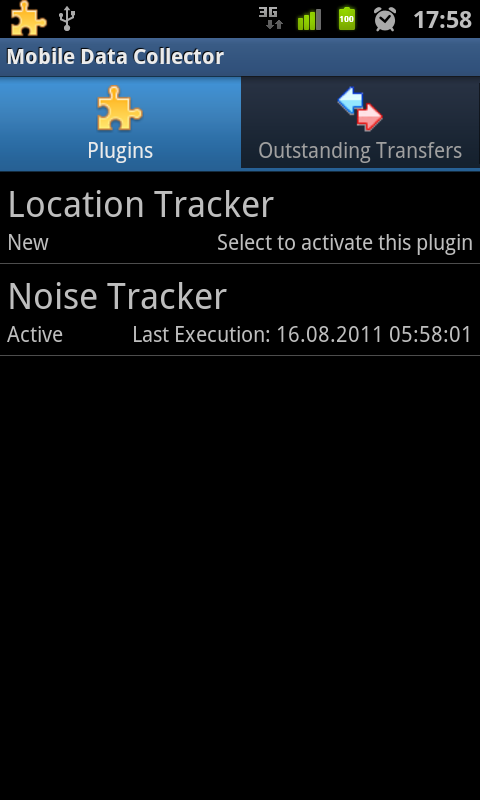
\includegraphics[width=5cm]{grafiken/active.png}
	\caption{Aktiviertes Plug-In}
	\label{activate}
\end{figure}

W�hlt man ein aktiviertes Plug-In erneut an, deaktiviert man es, wie in
Abbildung \ref{deactivated} zu sehen.

\begin{figure}[h!] 
	\centering
	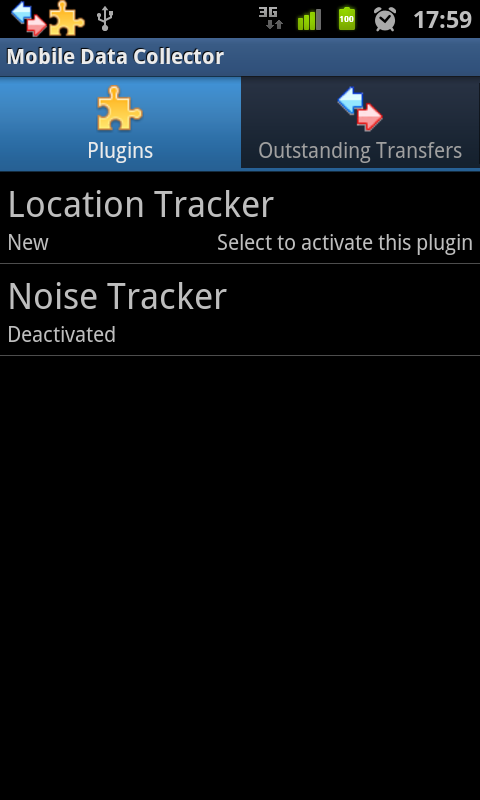
\includegraphics[width=5cm]{grafiken/deactivated.png}
	\caption{Deaktiviertes Plug-In}
	\label{deactivated}
\end{figure}

W�hlt man ein Plug-In durch ein langes Dr�cken aus, wird, wie in Abbildung
\ref{plugin_context_menu} dargestellt, das Kontextmen� angezeigt. Das
Kontextmen� erlaubt das Aktivieren und Deaktivieren eines Plug-Ins, das Anzeigen der Plug-In
Details (siehe hierzu Abschnitt \ref{plugin_details}) sowie das Deinstallieren
eines Plug-Ins.

\begin{figure}[h!] 
	\centering
	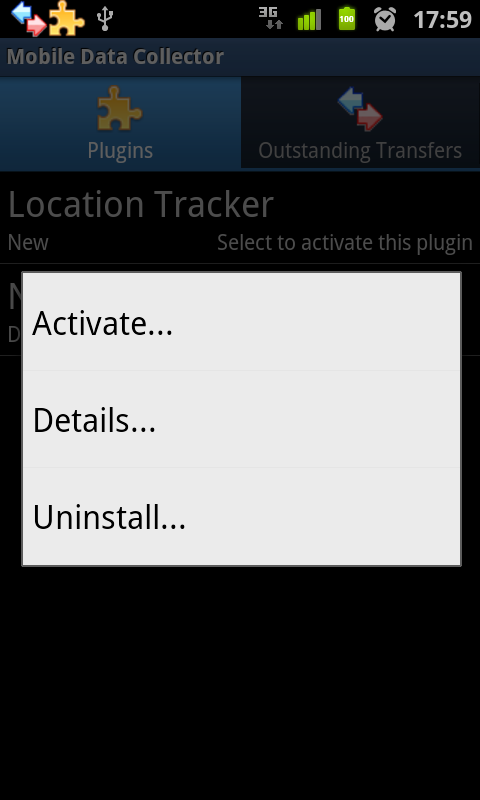
\includegraphics[width=5cm]{grafiken/plugin_context_menu.png}
	\caption{Context-Men� eines Plug-Ins}
	\label{plugin_context_menu}
\end{figure}

\subsection{Plug-In Details}
\label{plugin_details}
Der Benutzer hat �ber die {\em Plug-In Details} die M�glichkeit, zu jedem
Zeitpunkt, alle Informationen und Aktivit�ten eines Plug-Ins einzusehen. Die
{\em Plug-In Details} sind, wie im vorigen Abschnitt beschrieben, �ber das
Kontextmen� des Plug-Ins zu erreichen. �ffnet man die Details zu einem Plug-In,
werden die Plug-In-Informationen, wie in Abbildung \ref{details} angezeigt.
�ber die Tabs im oberen Bildschirmbereich gelangt man zu den weiteren Bereichen
{\em Logs} und {\em Collected Data}, die in den folgenden Abschnitten {\em
Log-Viewer} und {\em Data-Viewer} genauer erl�utert werden.

\begin{figure}[h!] 
	\centering
	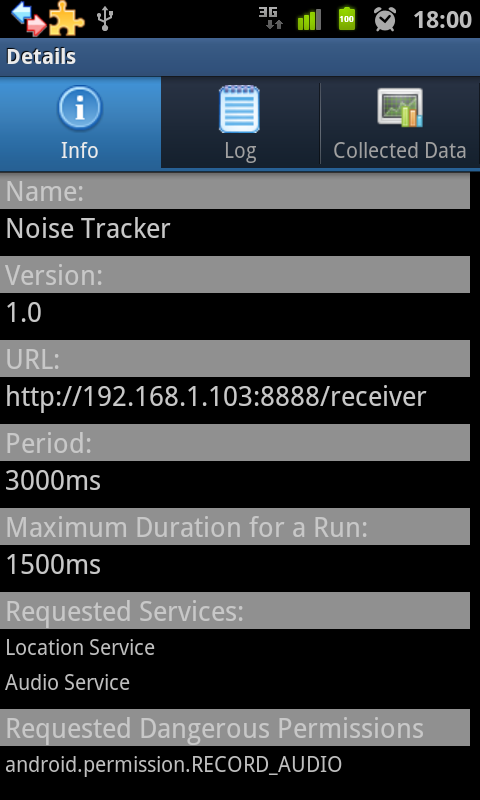
\includegraphics[width=5cm]{grafiken/details.png}
	\caption{Context-Men� eines Plug-Ins}
	\label{details}
\end{figure}

\subsubsection{Log-Viewer}
Der {\em Log-Viewer} dient zur Anzeige aller protokollierten Aktivit�ten eines
Plug-Ins. Mit Aktivit�ten ist der Zugriff auf die sicheren {\em Android System
Services} gemeint. Greift ein Plug-In auf eine Methode der Services zu, so wird
ein Log-Eintrag erstellt. Dieser gibt in benutzerverst�ndlicher Sprache an,
welche Informationen abgefragt wurden. Ein Beispiel ist in Abbildung \ref{log}
dargestellt. Der Log ist wie folgt aufgebaut. Jede Zeile zeigt an, wann das
Plug-In ausgef�hrt wurde. Durch die Auswahl eines Eintrags erweitern sich die
Eintr�ge um die eigentlichen Log-Eintr�ge. In diesem Fall sagen die Log-Eintr�ge
aus, dass am 16.08.2011 um 5:58:40 Uhr das Plug-In ausgef�hrt wurde. W�hrend
dieser Ausf�hrung wurde zur Lokalisierung des Benutzers das \acs{gsm}/\acs{umts}
Netz ({\em network}) verwendet und als Position wurden die Koordinaten am 53.8477729
L�ngengrad und am 10.6977904 Breitengrad ermittelt.

\begin{figure}[h] 
	\centering
	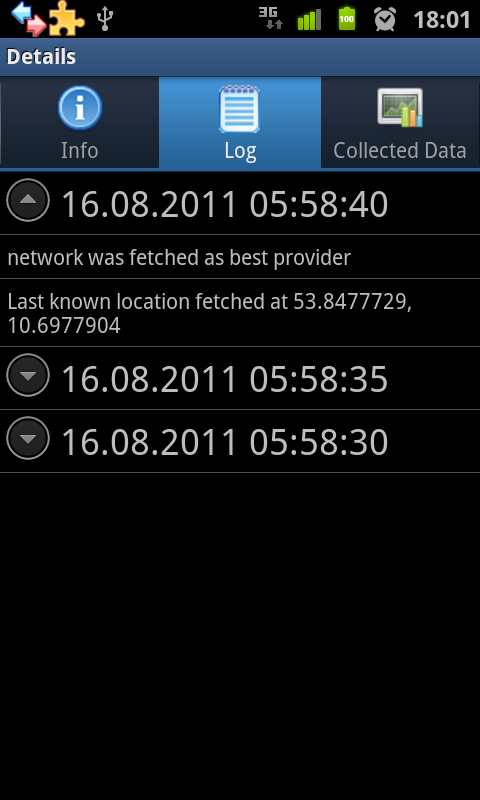
\includegraphics[width=5cm]{grafiken/log.png}
	\caption{Zugriffe aus die sicheren {\em Android System Services}}
	\label{log}
\end{figure}

\vspace*{1cm}

\subsubsection{Data-Viewer}
Der {\em Data-Viewer} dient zur Anzeige aller vom Plug-In gesammelten Daten bzw.
aller Daten, welche das Plug-In sp�ter �bertragen m�chte. Einem Plug-In steht es frei,
beliebig viele private Daten f�r interne Zwecke zu sammeln, diese lassen dann
aber nicht durch den {\em Mobile Data Collector} �bertragen.

Die im Konzept beschriebene hierarchische Datenstruktur l�sst sich durch den
{\em Data-Viewer} anzeigen. Dabei wird jede Ebene der Datenstruktur als Liste
dargestellt. In Abbildung \ref{collected_data_overview} wird die erste Ebene
angezeigt. Jeder anklickbare Knoten wird als Datum angezeigt. Das
Datum gibt an, wann der entsprechende Datensatz das letzte Mal modifiziert
wurde. In diesem Fall werden drei Eintr�ge dargestellt, die sich mit denen die
im Log stehen �berschneiden. Damit ist gemeint, dass nach jedem Zugriff auf den
{\em LocationManager}, ein neuer Eintrag zu den gesammelten Daten hinzugef�gt
wurde.

\begin{figure}[h] 
	\centering
	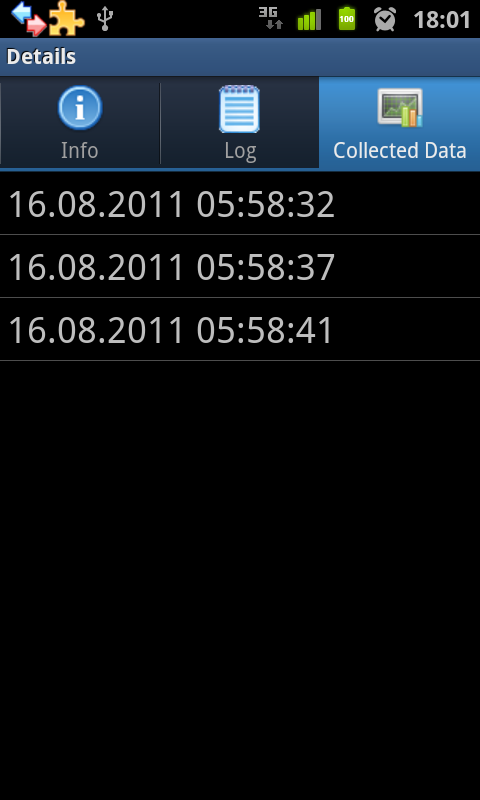
\includegraphics[width=5cm]{grafiken/collected_data_overview.png}
	\caption{Collected Data}
	\label{collected_data_overview}
\end{figure}

W�hlt man einen Knoten aus, so gelangt man in der Hierarchie eine
Ebene tiefer. Die unterhalb eines Knoten gespeicherten Daten k�nnen wie in
Abbildung \ref{collected_data_details} aussehen. In diesem Beispiel befinden sich auf
der angezeigten Ebene nur Eigenschaften. Die Eigenschaften beschreiben von
oben nach unten die H�he, Geschwindigkeit, Lautst�rke, L�ngengrad, Genauigkeit,
Breitengrad, Drehrichtung und die Art der Positionsbestimmung. Um wieder auf
eine h�here Ebene zu gelangen, kann die Zur�cktaste verwendet werden.

\begin{figure}[h] 
	\centering
	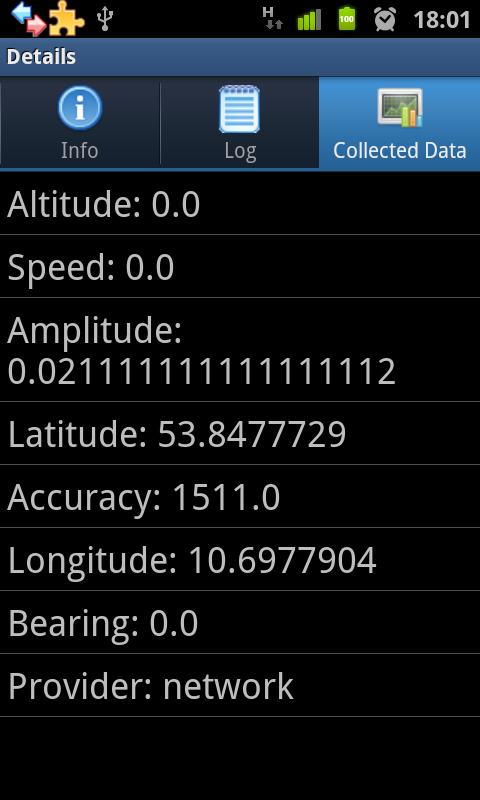
\includegraphics[width=5cm]{grafiken/collected_data_details.png}
	\caption{Gesammelte Daten eines Plug-Ins}
	\label{collected_data_details}
\end{figure}

\subsection{Transfer-Manager}
Der Transfer-Manager dient zur Verwaltung aller ausstehenden �bertragungen.
Sollte eine neue �bertragung ausstehen, so wird der Benutzer wie in Abbildung
\ref{new_transfer} dar�ber informiert.

\begin{figure}[h!] 
	\centering
	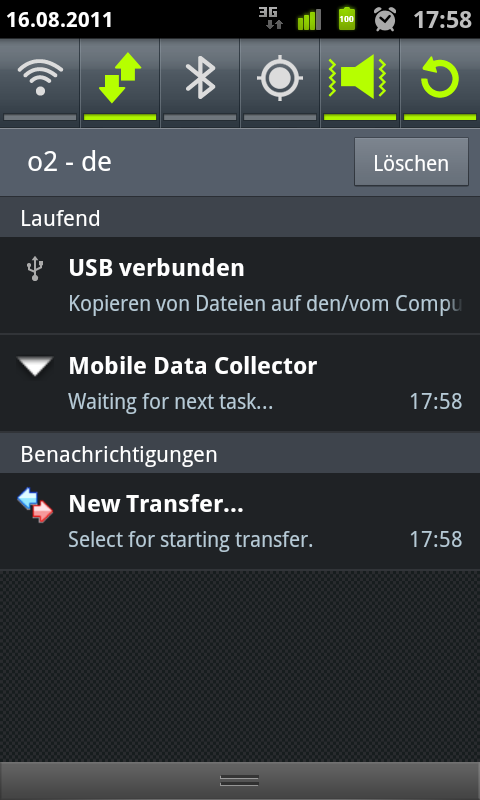
\includegraphics[width=5cm]{grafiken/new_transfer.png}
	\caption{Neue �bertragung}
	\label{new_transfer}
\end{figure}

Durch die Auswahl eines Eintrages gelangt der Benutzer in den
�bertragungsbereich des {\em Mobile Data Collectors}. Dieser kann bei einer
ausstehenden �bertragung wie in Abbildung \ref{transfer_pending} aussehen.

\begin{figure}[h!] 
	\centering
	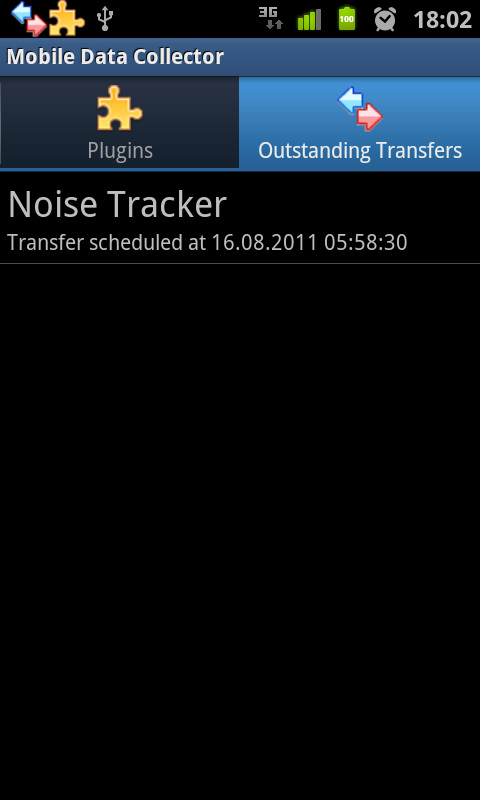
\includegraphics[width=5cm]{grafiken/transfer_pending.png}
	\caption{Ausstehende �bertragung}
	\label{transfer_pending}
\end{figure}

W�hlt der Benutzer den entsprechenden Eintrag aus, so gelangt er in die in
Abbildung \ref{transfer_details} dargestellte Detailansicht der �bertragung. In
dieser kann der Benutzer noch mal alle Informationen und Aktivit�ten des
Plug-Ins betrachten. Hierbei handelt es sich um einen Schnappschuss des aktuellen
Zustandes des Plug-Ins, den es hatte, als die �bertragung vorbereitet wurde.

\begin{figure}[h!] 
	\centering
	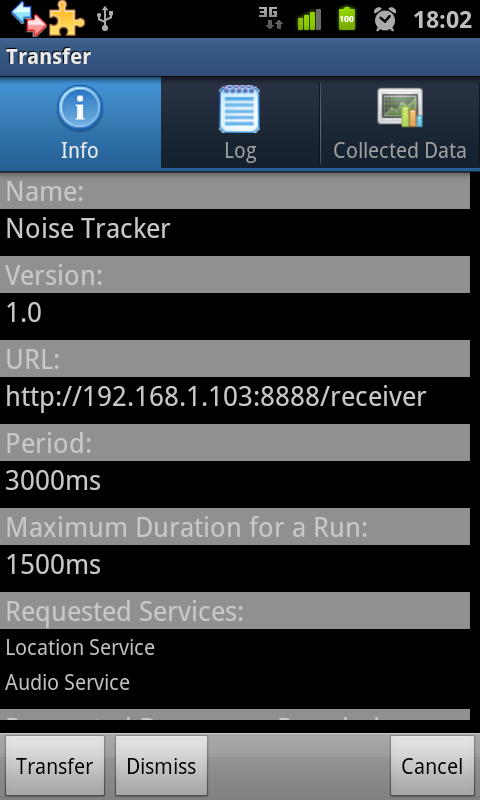
\includegraphics[width=5cm]{grafiken/transfer_details.png}
	\caption{�bertragungsdetails}
	\label{transfer_details}
\end{figure}

Hat der Benutzer alle Daten gesichtet und ist mit der �bertragung einverstanden,
kann er durch das Dr�cken der {\em Transfer}-Schaltfl�che die �bertragung
einleiten. Daraufhin wird dem Benutzer der Fortschritt der �bertragung, wie in
Abbildung \ref{transfer_details_sending} und \ref{transfer_sending_notification}
zu sehen, als Dialog und Mitteilung angezeigt.

\begin{figure}[h!] 
	\centering
	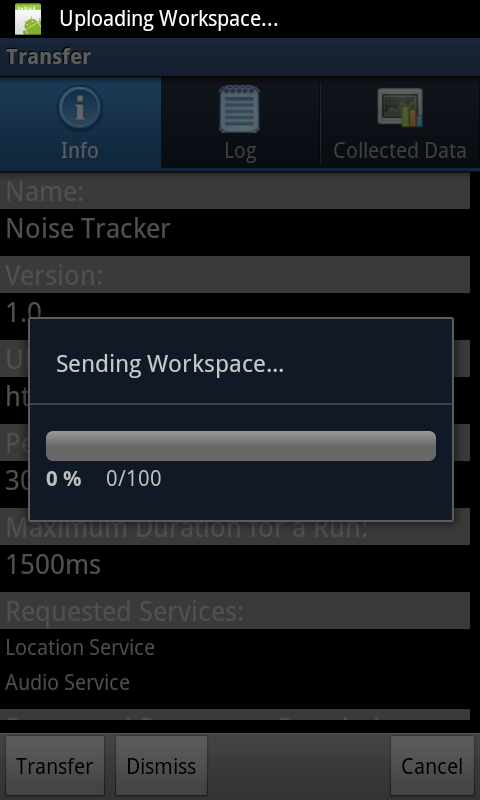
\includegraphics[width=5cm]{grafiken/transfer_details_sending.png}
	\caption{�bertragungsfortschritssdialog}
	\label{transfer_details_sending}
\end{figure}

\begin{figure}[h!] 
	\centering
	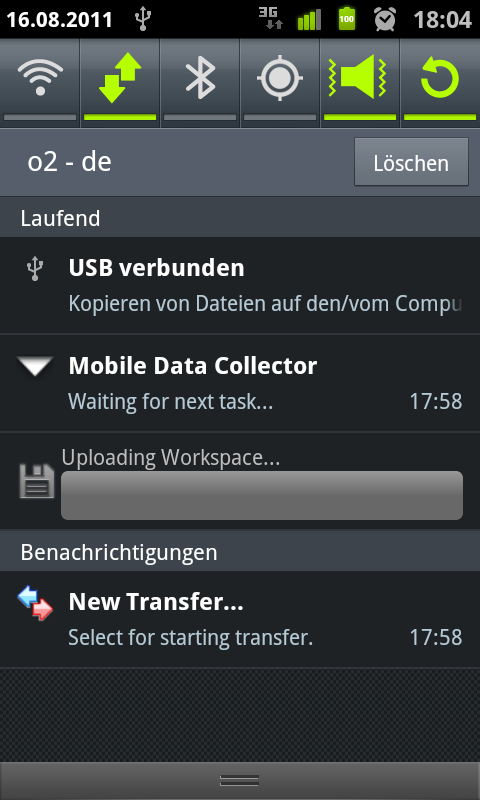
\includegraphics[width=5cm]{grafiken/transfer_sending_notification.png}
	\caption{�bertragungsfortschritt im Mitteilungsbereich}
	\label{transfer_sending_notification}
\end{figure}

Ist der Benutzer nicht mit der �bertragung seiner Daten einverstanden, kann er
durch die {\em Dismiss} Schaltfl�che, die �ber\-trag\-ung l�schen. Alle in der
�bertragung angezeigt Daten gehen daraufhin unwiderruflich verloren.

Intern wird bei der �bertragung zu einem Server eine \acs{http}-Verbindung
aufgebaut. Das Verbindungsziel wird hierbei dem \acs{url}-Attribut der
Plug-In-Informationen entnommen. Die Daten, die in Form von Java-Objekten
vorliegen, werden dann mithilfe der GSON-Bibliothek in ein \acs{json}-Objekt
�bersetzt~\cite{gson}. Da ein \acs{json}-Objekt sich optimal als Zeichenkette
abbilden l�sst, kann diese ohne gro�en Aufwand per \acs{http} versendet werden.

\section{Aufbau der Serverkomponente}
Durch die Serverkomponente soll ein Plug-In-Entwickler die M�glichkeit erhalten,
sehr schnell und einfach einen eigenen Server zu implementieren, um Daten von
einem Plug-In zu empfangen und zu verarbeiten. Die Serverkomponente steht als
Java-Bibliothek bereit und soll die einfache Integration in bestehende
Applikationsserver erlauben.

Die Serverkomponente ist wie folgt aufgebaut. Das {\em
TransferRequestReceiver}-Servlet empf�ngt die vom {\em Mobile Data Collector}
versandte \acs{json}-Datenstruktur und konvertiert diese in eine �quivalente
Java-Datenstruktur. Zur Konvertierung wird, wie auf dem Smartphone, die
GSON-Bibliothek verwendet. Die Java-Datenstruktur kann nun vom {\em
TransferRequestProzessor} weiter verarbeitet werden. Es wird empfohlen,
die sehr allgemeine empfangene Datenstruktur in eine spezifischere Datenstruktur
zu �berf�hren, die sich leichter verarbeiten und speichern l�sst. Wie die Daten
persistiert werden, muss der Entwickler selbst entscheiden.

Die Serverkomponente wurde mithilfe des \acf{di}
Frameworks {\em Google Guice}~\cite{guice} und dem Java-Build-Werkzeug
{\em Maven}~\cite{maven} entwickelt.

Beispiele einschlie�lich deren Implementierung sind im Kapitel
\ref{cha:evaluation} genauer beschrieben.

\section{Realisierungsprobleme}
\label{problemsofimplementation}
W�hrend der Realisierung des {\em Mobile Data Collectors} trat bei der
Entwicklung folgendes Problem auf. Auf viele, der von Android verwalteten
Hardware kann zwischen mehreren parallel laufenden Anwendungen konkurrierend
zugegriffen werden. Hardware wie z.~B. \acs{gps} oder der Lagesensor werden aus
jenem Gr�nden als {\em Android System Service} angeboten. Es gibt aber auch
Hardware, die nur von einer Anwendung zurzeit verwendet werden kann. Das sind
z.~B. die Kamera und das Mikrofon. Diese werden nicht als {\em Android System
Service} angeboten, sondern als Schnittstelle zu einer nativen Bibliothek,
welche die Hardware ansteuern kann.

{\em Android System Services} lassen sich sehr einfach durch eine neue
Implementierung ersetzen, weil es selbst zur Kommunikation mit der eigentlichen,
dahinter liegenden Service-Implementierung den \acs{ipc}-Mechanismus verwenden.
Das ist bei den Klassen zur Ansteuerung der Kamera und dem Mikrofon nicht der
Fall. Das Problem liegt darin, dass diese, die anfallenden Daten in Dateien
speichern. Man k�nnte nun die Klassen wie die {\em Android System Service} durch
eine sichere Implementierung ersetzen, indem man ebenfalls den
\acs{ipc}-Mechanismus verwendet, um die Ausf�hrung in den {\em Mobile Data
Collector} zu verschieben. Hierbei ergibt sich aber das Problem, dass die
aufgenommenen Daten in einer Datei im {\em Mobile Data Collector} gespeichert
werden. Die Datei w�re f�r ein Plug-In durch die Android-Sandbox-Architektur
nicht direkt zugreifbar. Hierf�r m�sste eine weitere Schnittstelle geschaffen
werden, um Plug-Ins den Zugriff auf die Datei zu erm�glichen. Auf diese L�sung
wurde zugunsten einer leichteren Implementierung von Plug-Ins verzichtet.
Stattdessen sollten in diesen F�llen die von Android zur Verf�gung gestellten
Implementierungen verwendet werden. Da der Zugriff auf Kamera und Mikrofon
ebenfalls durch {\em Permissions} geregelt wird, wird bei Aktivierung der
Benutzer darauf hingewiesen. Da die eigentlichen zu �bertragenden Daten
weiterhin zentral im {\em Mobile Data Collector} gespeichert werden m�ssen,
entf�llt hierbei nur die M�glichkeit der Protokollierung.

Das Problem lie�e sich am besten durch die Verwendung von \acs{osgi} l�sen.
Durch \acs{osgi} w�rden der {\em Mobile Data Collector} und alle Plug-Ins im
selben Prozess laufen. Dadurch w�rde sich der Zugriff auf Dateien deutlich
vereinfachen. Des Weiteren k�nnte man durch einen eigenen {\em ClassLoader} den
Zugriff auf bestimmte Klassen verbieten, sodass ein Entwickler dazu gezwungen
w�rde, die sicheren Implementierungen einer Klasse zu verwenden.

	\chapterfin
	\chapter{Leitfaden zur Plug-In Entwicklung}
\label{cha:leitfaden}
In diesem Kapitel wird erkl�rt, wie man mithilfe der Eclipse \acs{ide}, Plug-Ins
f�r den {\em Mobile Data Collector} entwickeln kann. Das schlie�t neben der
Entwicklung der Smartphone-Komponente auch die Serverkomponente ein. Das Kapitel
ist in drei Teile gegliedert. Im ersten wird erkl�rt, wie man die n�tigen
Frameworks zur Entwicklung von Plug-Ins, sowie deren Serverkomponente beziehen
kann. Im zweiten wird die Entwicklung eines einfachen Plug-Ins erkl�rt, und im
letzten die Entwicklung der dazugeh�rigen Serverkomponente. Das hierbei
entwickelte Plug-In tr�gt den Arbeitstitel ``Hallo Welt''-Plug-In. Das Plug-In
speichert bei jeder Ausf�hrung den Text ``Hallo Welt'' in der Datenstruktur des
{\em Mobile Data Collectors}. Dieses Kapitel verzichtet aus
Gr�nden der Einfachheit, auf die Verwendung von {\em Android System Services}.
Beispiele dazu k�nnen dem Abschnitt \ref{cha:evaluation} entnommen werden.

\section{Beziehen des Mobile Data Collection Frameworks}
Das {\em Mobile Data Collection Framework} kann entweder von der beiliegenden CD
oder von GitHub �ber die \acs{url} \url{https://github.com/mlegenhausen/mdcf}
bezogen werden. Das Framework kann als Archiv heruntergeladen oder per
Git geklont werden. Bei Git handelt es sich um ein verteiltes
Versionskontrollsystem, das von \url{http://git-scm.com/} heruntergeladen werden kann.

Um das Projekt per Git zu klonen, muss Folgendes auf der Kommandozeile
ausgef�hrt werden. Vor der Ausf�hrung sollte man sich in einem entsprechenden
Verzeichnis befinden, in das man das Projekt klonen m�chte.

\begin{lstlisting}[language=bash]
git clone git://github.com/mlegenhausen/mdcf.git
\end{lstlisting}

Nach dem Klonen kann man die aktuelle stabile Version aus der {\em
master}-Branch oder die Entwicklerversion aus dem {\em develop}-Branch verwenden. Nach dem
Klonen befindet man sich automatisch im {\em master}-Branch. Um in den {\em
develop}-Branch zu wechseln, muss Folgendes auf der Kommandozeile ausgef�hrt
werden.

\begin{lstlisting}[language=bash]
cd mdcf
git checkout develop
\end{lstlisting}

Das Framework zur Implementierung des Plug-Ins befindet sich im {\em
Mobile\-Data\-Collection\-Framework}-Verzeichnis, w�hrend sich das Framework zur
Implementierung der Serverkomponente im {\em mdcf-remote}-Verzeichnis befindet.

\section{Entwicklung eines Plug-Ins}
Die Entwicklung eines Plug-Ins wird im Folgenden anhand eines ``Hallo
Welt''-Plug-Ins dargestellt. Dabei wird der komplette Umfang der Entwicklung
beschrieben. Das schlie�t das Beziehen der n�tigen Software sowie deren
Einrichtung ein.

\subsection{Einrichtung der Entwicklungsumgebung Eclipse}
Der Autor empfiehlt die Verwendung der Eclipse \acs{ide}, da diese zum Zeitpunkt
der Arbeit die beste Unterst�tzung bei der Entwicklung von Android-Anwendungen
geboten hat. Zur Einrichtung der Eclipse \acs{ide} sind folgende Schritte
durchzuf�hren.

\begin{enumerate}
  \item Installation des Android-\acfp{sdk}. Dazu m�ssen
  die Schritte auf \url{http://developer.android.com/sdk/installing.html}
  befolgt werden.
  \item Installation des \acf{adt} Plug-In f�r Eclipse.
  Dazu m�ssen die Schritte auf
  \url{http://developer.android.com/sdk/eclipse-adt.html} befolgt werden.
\end{enumerate}

Die Entwicklungsumgebung ist nun vollst�ndig eingerichtet.

\subsection{Import des Mobile Data Collection Framework}
Bevor ein Plug-In entwickelt werden kann, muss das {\em Mobile Data Collection
Framework} und der {\em Mobile Data Collector} in den Workspace von Eclipse
importiert werden. Dazu geht man wie folgt vor. Durch einen Rechtsklick auf den
{\em Package Explorer} kann durch die Men�punkte {\em New} und {\em
Project\ldots} der {\em New Project}-Dialog ge�ffnet werden. In diesem w�hlt man
unter dem Verzeichnis {\em Android}, {\em Android Project} aus. Durch einen
Klick auf {\em Next} gelangt man zum {\em New Android Project}-Dialog. In diesem
Dialog w�hlt man {\em Create project from existing source} aus und setzt durch
{\em Browse\ldots} den Pfad zum {\em MobileDataCollectionFramework}-Verzeichnis,
das sich im {\em mdcf}-Verzeichnis befindet. Durch einen Klick auf {\em Finish}
wird das Projekt erstellt und das {\em Mobile Data Collection Framework} in den
Workspace importiert. Diese Schritte wiederholt man im Anschluss f�r das {\em
MobileDataCollector}-Verzeichnis. Sind beide Projekte importiert, kann das
eigentliche Plug-In erstellt werden.

\subsection{Erstellen des Plug-In Projekts}
Im ersten Schritt muss ein neues Android-Projekt erstellt werden. Das geschieht
mit Eclipse wie folgt. Durch einen Rechtsklick auf den {\em Package Explorer} kann
durch die Men�punkte {\em New} und {\em Project\ldots} der {\em New
Project}-Dialog ge�ffnet werden. In diesem w�hlt man unter dem Verzeichnis {\em
Android}, {\em Android Project} aus. Durch einen klick auf {\em Next} gelangt
man zum {\em New Android Project}-Dialog. In diesem Dialog tr�gt man unter {\em
Project name} ``HelloWorldPlugin'' ein. W�hlt unter {\em Build target} die
Android-Version 2.3.3 aus, gibt unter {\em Package name}
{\em com.example.helloworld} ein und w�hlt den Haken bei {\em Create Activity}
ab. Durch einen Klick auf {\em Finish} wird das Projekt erstellt.

Im n�chsten Schritt muss das {\em Mobile Data Collection Framework} zum Projekt
hinzugef�gt werden. Dazu muss man einen Rechtsklick auf das {\em
HelloWorldPlugin}-Projekt machen und den Men�punkt {\em Properties} ausw�hlen.
In dem sich �ffnen Dialog w�hlt auf der linken Seite den Punkt {\em Android}
aus. Dort kann man durch einen Klick auf {\em Add\ldots} das {\em
Mobile\-Data\-Collection\-Framework}-Projekt hinzuf�gen. Durch einen Klick auf
{\em OK} wird das Framework zum Plug-In hinzugef�gt.

Nachdem man das Framework hinzugef�gt hat, werden Fehler angezeigt. Um diese
Fehler zu beseitigen, muss die Simple-\acs{xml} Bibliothek zum Projekt
hinzugef�gt werden. Dazu erstellt man unterhalb des {\em HelloWorldPlugin}-Projekts ein
{\em lib}-Verzeichnis. In dieses kopiert man vom {\em lib}-Verzeichnis des {\em
Mobile\-Data\-Collection\-Framework}-Projekts die {\em simple-xml-2.5.3.jar}.
Danach muss die Bibliothek noch zum {\em Java Classpath} hinzugef�gt werden.
Dazu geht man wieder in die {\em Properties} des {\em HelloWorldPlugin}-Projekts. Auf
der linken Seite w�hlt man {\em Java Build Path} aus. Daraufhin w�hlt man den
Tab {\em Libraries} aus und klickt dort auf {\em Add Jars\ldots}. In dem sich �ffnen
Dialog navigiert man zu der zuvor kopierten Bibliothek und w�hlt diese aus.
Durch einen Klick auf {\em OK} wird die Bibliothek zum {\em Java Classpath}
hinzugef�gt und das Projekt ist fehlerfrei.

\subsection{Implementierung des Plug-Ins}
\label{pluginimplementation}
Nach der Erstellung des Projekts kann jetzt das eigentliche Plug-In
implementiert werden. Hierzu erstellt man im Package {\em
com.example.helloworld} eine Klasse mit dem Namen {\em HelloWorldPlugin}. Dazu
macht man einen Rechtsklick auf das Package und w�hlt {\em New} und {\em Class}
aus. Unter {\em Name} gibt man den Namen {\em HelloWorldPlugin} ein und bei {\em
Superclass} w�hlt man mit einem Klick auf Browse die Klasse {\em AbstractPlugin}
aus. Durch einen Klick auf {\em Finish} wird die Klasse wie in Listing
\ref{helloworldplugin} erstellt.

\begin{lstlisting}[label=helloworldplugin,
caption=HelloWorldPlugin.java, language=java] package com.example.helloworld;

import de.uniluebeck.itm.mdcf.AbstractPlugin;

public class HelloWorldPlugin extends AbstractPlugin {

	@Override
	protected void onRun() throws Exception {
		
	}
}
\end{lstlisting}

Als Beispiel soll bei jedem Aufruf des Plug-Ins, ein ``Hello World''
gespeichert werden. Dazu f�gt man zur {\em onRun}-Methode den Code von Listing
\ref{helloworldonrun} hinzu.

\begin{lstlisting}[label=helloworldonrun, caption=Inhalt der
{\em onRun}-Methode, language=java] 
PersistenceManager persist = getPersistenceManager();
Node workspace = persist.getWorkspace();

Node entry = new Node();
entry.setProperty("Value", "Hello World");
workspace.addNode(entry);

persist.save(workspace);
\end{lstlisting}

In Zeile 1 bis 2 wird der {\em Workspace} abfragt. An diesem wird in Zeile 4 bis
6, ein neuer Knoten ({\em Node}) mit einer Eigenschaft ({\em Property}) mit dem
Namen ``Value'' hinzugef�gt. In der letzten Zeile werden alle �nderungen am {\em Workspace}
wieder gespeichert.

\subsubsection{Implementierung des Broadcast Receivers}
Als n�chstes muss ein {\em Broadcast Receiver} implementiert werden, um das
Plug-In auffindbar und Plug-In-Informationen dem {\em Mobile Data Collector}
verf�gbar zu machen. Dazu erstellt man, im selben Package, eine Klasse {\em
HelloWorldRegister}, die von {\em XMLPluginRegister} erbt. Zu der Klasse f�gt
man einen {\em Constructor} hinzu, der auf die Datei ``plugin.xml'' verweist.
Die Datei enth�lt die Plug-In-Informationen im \acs{xml}-Format. Die
Klasse sollte danach wie in Listing \ref{helloworldregister} aussehen.

\begin{lstlisting}[label=helloworldregister,
caption=HelloWorldRegister.java, language=java]
package com.example.helloworld;

import de.uniluebeck.itm.mdcf.XMLPluginRegister;

public class HelloWorldRegister extends XMLPluginRegister {

	public HelloWorldRegister() {
		super("plugin.xml");
	}
}
\end{lstlisting}

Nun muss noch die zuvor genannte ``plugin.xml'' angelegt werden. Hierzu erstellt
man eine \acs{xml}-Datei im Package {\em com.example.helloworld}. Es ist darauf
zu achten, das sich die \acs{xml}-Datei innerhalb des {\em Java Classpath}
befindet. In die ``plugin.xml'' ist das Listing \ref{helloworldpluginxml} zu
kopieren.

\begin{lstlisting}[label=helloworldpluginxml, caption=plugin.xml, language=xml]
<plugininfo action="com.example.helloworld.HELLO_WORLD_PLUGIN" version="1.0">
	<name>Hello World</name> 
	<period>10000</period>
	<duration>1000</duration>
	<url>http://HOSTNAME:PORT/receiver</url>
	<transferInterval>600000</transferInterval>
</plugininfo>
\end{lstlisting}

In der Konfigurationsdatei wurden folgende Parameter festgelegt.

\begin{itemize}
  \item {\bf action}: Das Plug-In kann innerhalb des Android-Systems �ber die
  {\em action}\\ {\em com.example.helloworld.HELLO\_WORLD\_PLUGIN} per \acs{ipc} angesprochen
  werden.
  \item {\bf version}: Das Plug-In tr�gt die Version 1.0.
  \item {\bf name}: Der Darstellungsname innerhalb des {\em Mobile Data
  Collectors} ist ``Hello World''.
  \item {\bf period}: Das Plug-In wird alle 10.000ms bzw. alle 10s ausgef�hrt.
  \item {\bf duration}: Die maximale Ausf�hrungsdauer betr�gt 1.000ms. Wird
  die Zeit �ber\-schritten wird das Plug-In vom Android-System terminiert.
  \item {\bf url}: Alle gesammelten Daten sollen bei einer �bertragung an die
  \acs{url}\\ {\em http://HOSTNAME:PORT/receiver} gesendet werden.
  \item {\bf transferInterval}: Nach einer Zeit von 600.000ms bzw. 10min sollen
  alle Daten �bertragen werden. Das schlie�t nur die Zeit ein in der das Plug-In
  aktiv war.
\end{itemize}

Die Parameter k�nnen je nach Anforderung und Konfiguration beliebig abge�ndert
werden. Weitere m�gliche Konfigurationsparameter innderhalb des {\em
plugininfo}-Tags sind:

\begin{itemize}
  \item {\bf resetWorkspaceAfterTransfer}: Gibt an, ob der {\em Workspace}
  automatisch gel�scht werden soll, nachdem das Plug-In im {\em Transfer}-Mode
  war. Der {\em Workspace} wird standardm��ig nach der Erstellung einer
  �bertragung gel�scht.
  \item {\bf description}: Eine l�ngere Plug-In Beschreibung.
  \item {\bf services}: Gibt an, welche sicheren {\em Android System Services} bei der
  Plug-In Aus\-f�hrung gesetzt werden sollen.
\end{itemize}

Die zurzeit verf�gbaren sicheren {\em Android System Services} sind:

\begin{itemize}
  \item {\bf location}: Zur Anforderung des {\em LocationManager}, um die
  aktuelle Posi\-tion des Benutzers zu ermitteln.
  \item {\bf connectivity}: Zur Anforderung des {\em ConnectivityManager}, um
  den aktuellen Zustand der Netzwerkverbindung abzufragen.
  \item {\bf wifi}: Zur Anforderung des {\em WifiManager}, um Zugriff auf
  Wireless \acs{lan} zu erhalten.
  \item {\bf phone}: Zur Anforderung des {\em TelephonyManager}, um
  Informationen �ber alle Mobilfunkaspekte abzufragen.
\end{itemize}

Ein Beispiel f�r die Verwendung der Parameter ist in Lisiting
\ref{additionalparameters} dargestellt. In diesem werden alle verf�gbaren {\em
Android System Services} angefordert und der {\em Workspace} wird nach der
Erstellung einer �bertragung nicht mehr gel�scht.

\begin{lstlisting}[label=additionalparameters, caption=Zus�tzliche
Konfigurationsparameter, language=xml] 
<plugininfo action="..." version="1.0">
	...
	<services>
		<service>location</service>
		<service>wifi</service>
		<service>connectivity</service>
		<service>telephony</service>
	</services>
	<resetWorkspaceAfterTransfer>
		false
	</resetWorkspaceAfterTransfer>
	<description>
		This is an example Plug-In.
	</description>
	...
</plugininfo>
\end{lstlisting}

Ein konkretes Beispiel, indem die Konfigurationparameter verwendet werden,
kann dem Kapitel \ref{cha:evaluation} entnommen werden.

\subsubsection{Konfiguration der Manifest-Datei}
Zu guter Letzt muss das Plug-In und der {\em Broadcast Receiver} dem
Android-System bekannt gemacht werden. Dazu muss die {\em AndroidManifest.xml}
angepasst werden. Die Anpassungen sehen wie in Listing \ref{helloworldmanifest}
aus.

\begin{lstlisting}[label=helloworldmanifest, caption=AndroidManifest.xml,
language=xml] <?xml version="1.0" encoding="utf-8"?>
<manifest 
		xmlns:android="http://schemas.android.com/apk/res/android"
		package="com.example.helloworld"
		android:versionCode="1" android:versionName="1.0">	
	<application 
			android:icon="@drawable/icon" 
			android:label="@string/app_name">
		<receiver 
				android:name="com.example.helloworld.HelloWorldRegister">
			<intent-filter>
				<action 
						android:name="de.uniluebeck.itm.mdcf.PLUGIN_FIND"/>
			</intent-filter>
		</receiver>
		<service 
				android:name="com.example.helloworld.HelloWorldPlugin">
			<intent-filter>
				<action 
						android:name="com.example.helloworld.HELLO_WORLD_PLUGIN"/>
			</intent-filter>
		</service>
	</application>
</manifest>
\end{lstlisting}

Die von Eclipse generierte {\em AndroidManifest.xml} wurde hierbei um zwei
Eintr�ge erweitert. Einmal um einen {\em Broadcast Receiver} (Zeile 8 bis 14)
und dem Plug-In, der als {\em Service} definiert wird (Zeile 15 bis 21). Der
{\em Broadcast Receiver} besitzt eine {\em action} mit dem Namen {\em
de.uniluebeck.itm.mdcf.PLUGIN\_FIND}. Durch diesen wird der {\em Broadcast
Receiver} aufgerufen, wenn der {\em Mobile Data Collector} nach Plug-Ins sucht.
Das Plug-In wiederum besitzt eine {\em action} mit dem Namen {\em
com.example.helloworld.HELLO\_WORLD\_PLUGIN}. Durch diese kann der {\em Mobile
Data Collector}, die Plug-In-Schnittstelle aufrufen und das Plug-In ausf�hren.
Hierbei ist darauf zu achten, dass die {\em action} denselben Wert besitzt wie
der {\em action}-Parameter in der ``plugin.xml'', da sonst das Plug-In nicht
ausgef�hrt werden kann.

\subsection{Plug-In installieren und ausf�hren}
Das Plug-In ist nun fertig und kann zum ersten Mal ausgef�hrt werden. Dazu muss
im ersten Schritt der {\em Mobile Data Collector} installiert werden. Das
geschieht durch einen Rechtsklick auf das {\em Mobile\-Data\-Collector}-Projekt.
Durch einen Klick im Kontextmen� auf {\em Run As} und {\em Android Application}
wird der {\em Mobile Data Collector} installiert. Sollte ein Android Smartphone am
Computer angeschlossen sein, so wird der {\em Mobile Data Collector} auf diesem
automatisch installiert. Sollte das nicht der Fall sein, wird der
Android-Emulator gestartet. Es ist zu Empfehlen den {\em Mobile Data Collector}
auf einem Smartphone zu installieren, da nur auf diesem, die volle Sensorik zur
Verf�gung steht. Nach der Installation wird der {\em Mobile Data Collector}
automatisch gestartet.

Im n�chsten Schritt kann jetzt das eigentliche Plug-In installiert werden. Dazu
installiert man das {\em Hello\-World\-Plugin} wie zuvor den {\em Mobile Data
Collector}. Nach der Installation wird das Plug-In in der Plug-In Liste des {\em
Mobile Data Collectors} angezeigt. Aktiviert man das Plug-In, wird
dieses, dass erste mal ausgef�hrt. Man kann sich nun in den Plug-In Details die
gespeicherten Daten anschauen. Navigiert man sich durch die Datenstruktur, so
wird man feststellen, dass bei jeder Ausf�hrung die Zeichenkette ``Hello World''
gespeichert wurde.

\section{Entwicklung der Serverkomponente}
Im Folgenden wird beschrieben, wie die Daten vom zuvor entwickelten Plug-In
empfangen und serverseitig weiter verarbeitet werden k�nnen. F�r die Entwicklung
der Serverkomponente kann eine beliebige \acs{ide} verwendet werden. Zum Bauen
des Projektes wird in diesem Fall {\em Maven} verwendet~\cite{maven}.

Da die Kommunikation mit dem {\em Mobile Data Collector} �ber das
\acs{http}-Pro\-to\-koll stattfindet, wird die Serverkomponente als
Web-Anwendung entwickelt. Hierzu werden normale Java Servlets verwendet, sowie das
\acs{di}-Framework {\em Google Guice}~\cite{guice}.

\subsection{Installation des Remote Frameworks}
Das {\em Remote Framework} dient zur einfachen Implementierung der
Serverkomponente. Es kann mit {\em Maven} wie folgt gebaut werden.

\begin{lstlisting}[language=bash]
cd mdcf-remote
mvn package
\end{lstlisting}

Unterhalb des {\em target}-Verzeichnisses befindet sich nun die fertig gebaute
Bibliothek, die in den folgenden Schritten verwendet wird.

\subsection{Erstellen des Projekts}
Um mit Maven ein Projekt zu erstellen, ist folgendes auf der Kommandozeile
auszuf�hren.

\begin{lstlisting}[language=bash]
mvn archetype:generate \
	-DgroupId=com.example.helloworld \
	-DartifactId=server \
	-Dversion=0.1-SNAPSHOT \
	-Dpackage=com.example.helloworld.server \
	-DarchetypeArtifactId=maven-archetype-webapp
\end{lstlisting}

Alle auftretenden Fragen k�nnen durch die Eingabe von {\em Enter} best�tigt
werden. Leider wird das Projekt unvollst�ndig von {\em Maven} generiert.
Deswegen wird f�r die weiteren Schritte empfohlen nachtr�glich ein {\em
src/main/java}-Verzeichnis hinzuzuf�gen sowie ein {\em
com.example.helloworld.server}-Package.

Bevor mit der eigentlichen Implementierung begonnen werden kann, m�ssen noch
die in Listing \ref{pomxml} angegebenen Abh�ngigkeiten zur {\em pom.xml}
hinzugef�gt werden.

\begin{lstlisting}[label=pomxml, caption=pom.xml, language=xml] 
<dependencies>
	<dependency>
		<groupId>de.uniluebeck.itm</groupId>
		<artifactId>mdcf-remote</artifactId>
		<version>0.1-SNAPSHOT</version>
		<scope>system</scope>
		<systemPath>
			${basedir}/lib/mdcf-remote-0.1-SNAPSHOT.jar
		</systemPath>
	</dependency>
	<dependency>
		<groupId>com.google.inject</groupId>
		<artifactId>guice</artifactId>
		<version>3.0</version>
	</dependency>
	<dependency>
		<groupId>com.google.inject.extensions</groupId>
		<artifactId>guice-servlet</artifactId>
		<version>3.0</version>
	</dependency>
</dependencies>
\end{lstlisting}

Hierbei wird als erstes das {\em Remote Framework} als Abh�ngigkeit definiert,
als zweites {\em Google Guice} und als letztes eine Erweiterung um {\em Google
Guice} mit Servlets zu verwenden.

\subsection{Implementierung der Serverkomponente}
Um die vom Smartphone empfangenen Daten zu verarbeiten, muss ein {\em
TransferRequestProcessor} implementiert werden. Dieser bekommt beim Aufruf der
{\em process}-Methode, den deserialisierten {\em TransferRequest}
�bergeben, der vom {\em Mobile Data Collector} �bertragen wurde. Siehe hierzu
Listing \ref{transferrequestprocessor}.

\begin{lstlisting}[label=transferrequestprocessor,
caption=TransferRequestProessorImpl.java, language=java] 
package com.example.helloworld.server;

import java.util.Iterator;

import de.uniluebeck.itm.mdcf.remote.TransferRequestProcessor;
import de.uniluebeck.itm.mdcf.remote.model.Node;
import de.uniluebeck.itm.mdcf.remote.model.TransferRequest;

public class TransferRequestProcessorImpl implements TransferRequestProcessor {

	public void process(TransferRequest request) {
		String id = request.getId();
		Node workspace = request.getWorkspace();
		Iterator<Node> nodes = workspace.getNodes();
		while (nodes.hasNext()) {
			Node node = nodes.next();
			String value = node.getProperty("Value").getValue()
				.getString();
			System.out.println("Participant-ID: " + id + ", Value: " + value);
		}
	}
}
\end{lstlisting}

In diesem Listing werden die vom {\em HelloWorldPlugin} empfangenen Daten
einfach auf der Konsole ausgegeben. Die in Zeile 12 angegebene ID ist die
eindeutige Benutzernutzerkennung des Smartphone-Besitzers und kann dazu
verwendet werden, Datens�tze einzelnen Benutzern zuzuordnen.

Damit der zuvor implementierte {\em TransferRequestProcessor} �ber eine
\acs{url} aufgerufen werden kann. Muss dieser noch unter Zuhilfenahme von {\em Google
Guice} konfiguriert werden. Hierzu ist ein {\em GuiceServletContextListener} zu
implementieren. Siehe hierzu Listing \ref{helloworldcontextlistener}.

\begin{lstlisting}[label=helloworldcontextlistener,
caption=HelloWorldContextListener.java, language=java] 
package com.example.helloworld.server;

import com.google.inject.Guice;
import com.google.inject.Injector;
import com.google.inject.servlet.GuiceServletContextListener;
import com.google.inject.servlet.ServletModule;

import de.uniluebeck.itm.mdcf.remote.MdcfRemoteModule;
import de.uniluebeck.itm.mdcf.remote.TransferRequestReceiver;

public class HelloWorldContextListener extends GuiceServletContextListener {

	@Override
	protected Injector getInjector() {
		return Guice.createInjector(new ServletModule() {
			@Override
			protected void configureServlets() {
				install(
					new MdcfRemoteModule(TransferRequestProcessorImpl.class));
				serve("/receiver").with(TransferRequestReceiver.class);
			}
		});
	}
}
\end{lstlisting}

In dem {\em HelloWorldContextListener} wird ein {\em ServletModule} definiert.
Dieses definiert zum einen, dass das installierte {\em MdcfRemoteModule} den
zuvor implementierten {\em TransferRequestProcessor} verwenden soll und dass die
Daten �ber das \acs{url}-Suffix {\em /receiver} empfangen werden k�nnen. Bei dem
{\em TransferRequestReceiver} handelt es sich um ein Servlet, dass die vom Smartphone
empfangenen Daten, auf das {\em TransferRequest}-Objekt �bertr�gt und an den
definierten {\em TransferRequestProcessor} �bergibt. Hierbei ist anzumerken,
dass der Suffix mit der in Listing \ref{helloworldpluginxml} definierten {\em
url} �bereinstimmen muss. Letztendlich muss in der ``plugin.xml'' die \acs{url}
stehen, unter der das hier definierte Servlet erreichbar ist.

Damit das zuvor definierte {\em ServletModule} vom Servlet Container gefunden
werden kann, muss noch der {\em HelloWorldContextListener} �ber die {\em
web.xml} dem Servlet-Container bekannt gemacht werden. Das ist in Listing
\ref{webxml} dargestellt.

\begin{lstlisting}[label=webxml, caption=web.xml, language=xml] 
<?xml version="1.0" encoding="UTF-8"?>
<!DOCTYPE web-app
	PUBLIC "-//Sun Microsystems, Inc.//DTD Web Application 2.3//EN"
	"http://java.sun.com/dtd/web-app_2_3.dtd">

<web-app>

	<filter>
		<filter-name>guiceFilter</filter-name>
		<filter-class>
			com.google.inject.servlet.GuiceFilter
		</filter-class>
	</filter>

	<filter-mapping>
		<filter-name>guiceFilter</filter-name>
		<url-pattern>/*</url-pattern>
	</filter-mapping>
	
	<listener>
		<listener-class>
			com.example.helloworld.server.HelloWorldContextListener
		</listener-class>
	</listener>
	
	<welcome-file-list>
		<welcome-file>index.html</welcome-file>
	</welcome-file-list>

</web-app>
\end{lstlisting}

Die Serverkomponente ist jetzt komplett. Durch ein {\em mvn install} kann das
Projekt gebaut werden. Dabei wird im {\em target}-Verzeichnis ein {\em
WAR}-Archive erstellt. Dieses l�sst sich in einem beliebigen Servlet-Container
ausf�hren. F�hrt man die Serverkomponente aus und �bertragt Daten vom {\em
Mobile Data Collector} zum Server, wird man feststellen, dass auf der Console des Servers
die eindeutige Benutzerkennung und der Wert ``Hello World'' ausgegeben wird.

	\chapterfin
	\chapter{Evaluation}
\label{cha:evaluation}
In diesem Kapitel wird gezeigt, dass sich mithilfe des {\em Mobile Data
Collection Frameworks} auch komplexere Plug-Ins zum Sammeln von Sensordaten
entwickeln lassen. Das wird anhand zweier Beispiele gezeigt. Das erste Beispiel
ist ein Plug-In zur Positionverfolgung des Benutzers. Das zweite Beispiel ist
eine Erweiterung des Ersten bei der Zus�tzlich noch die Umgebungslautst�rke zu
jeder Position erfasst wird. Hierbei wird neben den Plug-Ins
f�r den {\em Mobile Data Collector} auch eine entsprechende Serverkomponente
entwickelt. Die Serverkomponente besteht aus der Persistierung
sowie der Visualisierung der Daten in Form einer Web-Anwendung.

\section{Plug-In zur Positionsverfolgung}
\label{locationtracker}
Aufbauend auf dem in Kapitel \ref{cha:leitfaden} beschriebenen ``Hallo Welt''-
Plug-In, wurde ein Plug-In entwickelt, dass die aktuelle Position
des Benutzers speichert und in regelm��igen Abst�nden �bertragt. Das Plug-In
tr�gt den Arbeitstitel {\em Location Tracker}. Es wird im Folgenden auf die
wichtigsten Punkte bei der Implementierung eingegangen.

\subsection{Implementierung des Plug-Ins}
Das Plug-In befindet sich im {\em LocationTrackerPlugin}-Verzeichnis des {\em
Mobile Data Collection Framework}-Projekts. Es wird sich im Folgenden, auf dem
im Verzeichnis befindlichen Quellcode bezogen.

\subsubsection{Ermittelung der aktuellen Position}
Um die aktuelle Position des Benutzers zu erfahren, muss der {\em
LocationManager} abgefragt werden. Siehe hierzu Listing \ref{locationmanager}

\begin{lstlisting}[label=locationmanager,
caption=Abfragen des LocationManager, language=java]
String provider = getLocationManager().getBestProvider(
	new Criteria(), false);
Location location = getLocationManager()
	.getLastKnownLocation(provider);
\end{lstlisting}

In Zeile 1 wird die Methode ermittelt, mit der die Position des Benutzers am
genausten bestimmt werden kann. Die Positionsermittlung wird innerhalb von
Android durch einen {\em Provider} bewerkstelligt. In diesem Fall soll ein
{\em Provider} ermittelt werden, der am Besten dem gegebenen {\em
Criteria}-Objekt entspricht. Durch das Objekt k�nnen Kriterien wie z.~B. Stromverbrauch und Genauigkeit
festgelegt werden. �bergibt man ein nicht weiter konfiguriertes Objekt, so wird
der zurzeit beste verf�gbare {\em Provider} zur�ckgegeben. In Zeile 2 wird
daraufhin die letzte bekannte Position unter Zuhilfenahme des gegebenen {\em
Providers} ermittelt. Das zur�ckgegebene {\em Location}-Objekt beschreibt die aktuelle
Position des Benutzers.

\subsubsection{Speichern der Position}
Die zuvor ermittelte Position kann nun gespeichert werden. In Listing
\ref{storelocation} wird dazu im ersten Schritt der {\em Workspace} abgefragt.
Dann wird eine neuer Knoten erstellt, an der alle Attribute des {\em
Location}-Objekts gespeichert werden. Der Knoten wird im letzten Schritt an den
{\em Workspace} angeh�ngt und gespeichert.

\begin{lstlisting}[label=storelocation,
caption=Speichern der Position, language=java]
Node workspace = getPersistenceManager().getWorkspace();
Node node = new Node();
node.setProperty("Latitude", location.getLatitude());
node.setProperty("Longitude", location.getLongitude());
node.setProperty("Altitude", location.getAltitude());
node.setProperty("Bearing", location.getBearing());
node.setProperty("Accuracy", location.getAccuracy());
node.setProperty("Speed", location.getSpeed());
node.setProperty("Provider", location.getProvider());
workspace.addNode(node);
getPersistenceManager().save(workspace);
\end{lstlisting}

\subsubsection{Plug-In Konfiguration}
Um das Plug-In fertigzustellen, muss es im letzten Schritt konfiguriert werden.
Das geschieht ebenfalls �ber die {\em plugin.xml}. Eine m�gliche Konfiguration
ist in Listing \ref{locationtrackerpluginxml} dargestellt. Die Konfiguration
unterscheidet sich zum ``Hallo Welt''-Plug-In dadurch, dass der {\em
LocationManager} angefordert wird und eine Beschreibung angegeben ist. Der {\em
LocationManager} wird zur Ermittlung der aktuellen Position ben�tigt. Es ist
darauf zu achten, dass die angegebene \acs{url} mit der des Empfangsserver
�bereinstimmt.

\begin{lstlisting}[label=locationtrackerpluginxml, caption=plugin.xml,
language=xml] 
<plugininfo action="de.uniluebeck.itm.mdcf.plugin.locationtracker.LOCATION_TRACKER_PLUGIN" version="1.0">
	<name>Location Tracker</name>
	<period>10000</period>
	<duration>1000</duration>
	<url>http://HOSTNAME:PORT/receiver</url>
	<transferInterval>10000</transferInterval>
	<services>
		<service>location</service>
	</services>
	<description>
		Plugin that tracks every 10 seconds the current location.
	</description>
</plugininfo>
\end{lstlisting}

\subsubsection{Verwendung des Plug-Ins}
Das Plug-In kann jetzt, wie in Kapitel \ref{cha:leitfaden} beschrieben, auf dem
Smartphone installiert und ausgef�hrt werden. Nach der ersten Ausf�hrung k�nnen
wie in Abbildung \ref{log_locationtracker},
\ref{collected_data_overview_locationtracker} und
\ref{collected_data_details_locationtracker} zu sehen, die Zugriffe
auf den {\em LocationManager} sowie alle gesammelten Daten eingesehen werden.
Betrachtet man die gesammelten Daten des Plug-Ins wird man feststellen, dass die
zuvor definierte Datenstruktur mit den entsprechenden Positionsdaten gef�llt
wurde.

\begin{figure}[h] 
	\centering
	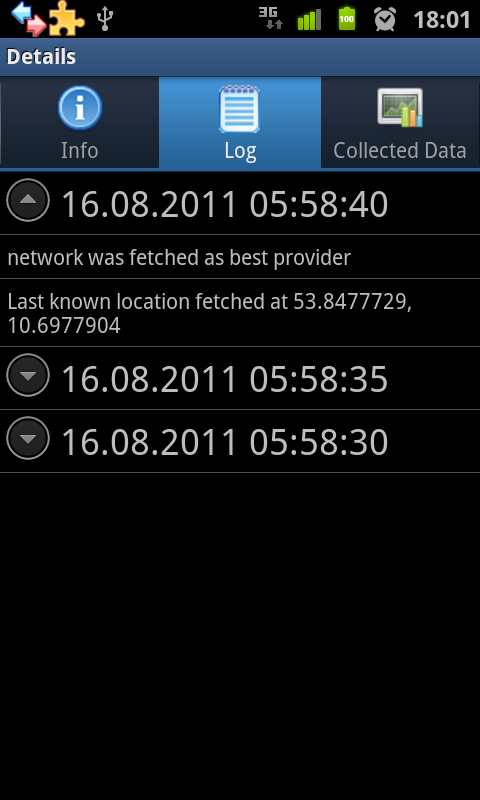
\includegraphics[width=5cm]{grafiken/log.png}
	\caption{Zugriffsprotokoll auf den LocationManager}
	\label{log_locationtracker}
\end{figure}

\begin{figure}[h] 
	\centering
	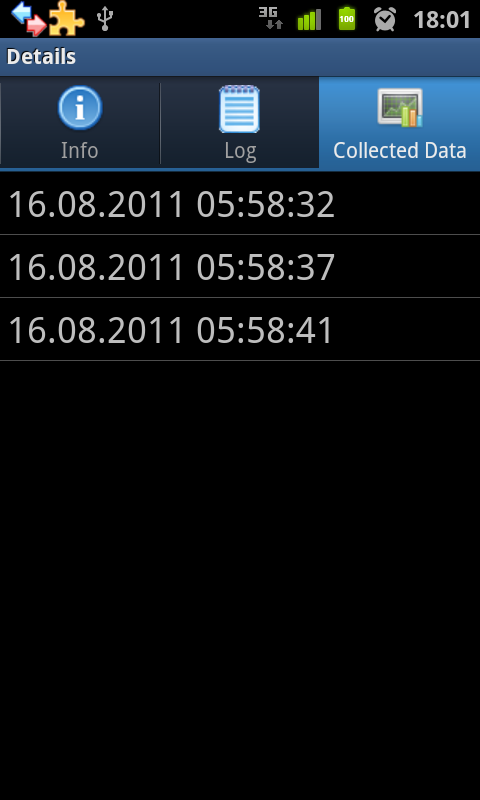
\includegraphics[width=5cm]{grafiken/collected_data_overview.png}
	\caption{�berblick �ber alle gesammelten Positionen}
	\label{collected_data_overview_locationtracker}
\end{figure}

\begin{figure}[h] 
	\centering
	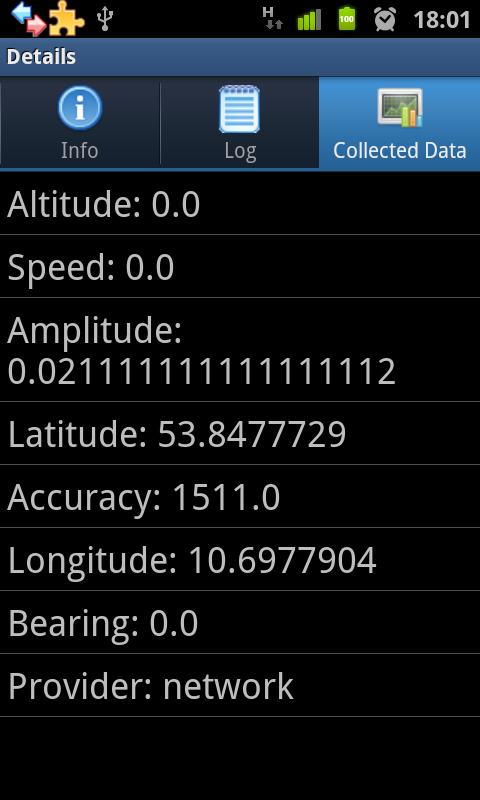
\includegraphics[width=5cm]{grafiken/collected_data_details.png}
	\caption{Detailierte Ansicht einer Position}
	\label{collected_data_details_locationtracker}
\end{figure}

Das Plug-In demonstriert somit, dass es mit dem {\em Mobile Data
Collection Framework} m�glich ist, Plug-Ins zu entwickeln, die
Positionsdaten sammeln k�nnen. Im n�chsten Abschnitt wird gezeigt, wie die
gesammelten Daten von einem Server empfangen, verarbeitet und visualisiert
werden k�nnen.

\subsection{Implementierung der Serverkomponente}
Bei der Implementierung der Serverkomponente wird als Ausgangspunkt die ``Hallo
Welt''-Serverkomponente verwendet. Diese wurde um eine Persistierungsschicht
erweitert und erlaubt die Visualisierung der Daten mit Hilfe einer
Web-Anwendung. Diese befindet sich im {\em
mdcf-locationtracker-remote}-Verzeichnis, des {\em Mobile Data
Collector}-Projektes.

\subsubsection{Persistierung der Daten}
Wie in Kapitel \ref{cha:leitfaden} beschrieben, werden die Daten nach dem
Empfang, an einen {\em TransferRequestProcessor} �bergeben. In der Klasse kann
z.~B. die Persistierung der Daten stattfinden. Bevor diese gespeichert
werden, sollte aber eine �berf�hrung des allgemeinen Datenformats des {\em Mobile Data Collection
Frameworks} in ein dom�nenspezifisches stattfinden. Eine �berf�hrung
des allgemeinen Datenformats in ein dom�nenspezifisches sowie die anschlie�ende
Speicherung kann wie in Listing \ref{datenmapping} implementiert werden.

\begin{lstlisting}[label=datenmapping,
caption=TransferRequestProcessorImpl.java, language=java] 
package de.uniluebeck.itm.mdcf.remote.locationtracker.server;

import java.util.Iterator;
import java.util.List;

import com.google.common.base.Objects;
import com.google.inject.Inject;

import de.uniluebeck.itm.mdcf.remote.TransferRequestProcessor;
import de.uniluebeck.itm.mdcf.remote.locationtracker.server.domain.Location;
import de.uniluebeck.itm.mdcf.remote.locationtracker.server.domain.Participant;
import de.uniluebeck.itm.mdcf.remote.model.Node;
import de.uniluebeck.itm.mdcf.remote.model.TransferRequest;

public class TransferRequestProcessorImpl implements TransferRequestProcessor {
	
	private final ParticipantRepository repository;
	
	@Inject
	public TransferRequestProcessorImpl(
			ParticipantRepository repository) {
		this.repository = repository;
	}
	
	public void process(TransferRequest request) {
		String id = request.getId();
		Participant participant = Objects.firstNonNull(
			repository.findById(id), new Participant(id));
		
		Node workspace = request.getWorkspace();
		Iterator<Node> nodes = workspace.getNodes();
		List<Location> locations = participant.getLocations();
		while (nodes.hasNext()) {
			Node node = nodes.next();
			Location location = new Location();
			location.setTimestamp(node.getTimestamp());
			location.setLatitude(node.getProperty("Latitude")
				.getValue().getDouble());
			location.setLongitude(node.getProperty("Longitude")
				.getValue().getDouble());
			location.setAltitude(node.getProperty("Altitude")
				.getValue().getDouble());
			location.setBearing((float) node.getProperty("Bearing")
				.getValue().getDouble());
			location.setAccuracy((float) node.getProperty("Accuracy")
				.getValue().getDouble());
			location.setSpeed((float) node.getProperty("Speed")
				.getValue().getDouble());
			location.setProvider(node.getProperty("Provider")
				.getValue().getString());
			locations.add(location);
		}
		repository.persist(participant);
	}
}
\end{lstlisting}

In diesem Listing wird gezeigt, wie der empfangene {\em TransferRequest} auf
ein {\em Participant}-Objekt �bertragen werden kann. Ein {\em Participant}
stellt einen Benutzer des {\em Mobile Data Collector} dar. Die
Identifikation findet anhand der eindeutigen Benutzerkennung statt, welche �ber
die {\em getId}-Methode abgefragt werden kann. Sollte der {\em Participant}
bereits existierten, werden die gesammelten Daten an den bereits existierenden
Benutzer angeh�ngt, da andernfalls ein neuer {\em Participant} erstellt wird.
Das {\em PersistentRepository} stellt die Datenbankabstraktionsschicht dar. In den darauf
folgenden Schritten werden die Daten aus dem {\em TransferRequest} an ein
entsprechendes {\em Location}-Objekt �bergeben und der {\em Participant} wird
gespeichert. Die Daten sind nun in einer Datenbank persistiert und stehen somit
anderen Anwendungen zur Verf�gung. In diesem Beispiel wurde zur Persistierung
der \acs{orm} {\em Hibernate} verwendet. Die Persistierungsmethode wird vom {\em
ParticipantRepsitory} abstrahiert. Durch die Abstraktion steht es dem Entwickler
frei, ein beliebiges anderes Persistierungsframework zu verwenden.

\subsubsection{Visualisierung der Daten}
Als letzter Teil der Evaluation sollen die gespeicherten Daten visualisiert
werden. Da es sich um Positionsdaten handelt, bietet es sich an, die
Positionen eines Benutzers auf einer Karte zu visualisieren. Dadurch ist die
Evaluierung der Daten sehr einfach.

F�r die technische Realisierung bietet es sich an, auf bereits bestehende
Infrastruktur und Programmiersprachen zur�ckzugreifen. Da bisher nur die
Programmiersprache Java verwendet wurde und bereits ein Java Servlet-Container
zum Empfang der Daten vorhanden ist, eignet sich ein javabasiertes
Web-Framework am besten. In diesem Fall fiel die Wahl auf
das {\em \acf{gwt}}~\cite{gwt}. Bei \acs{gwt} handelt es sich um einen
Java-zu-JavaScript-Compiler, der die Implementierung von Web-Anwendung in Java
erlaubt. Die clientseitige Ausf�hrung der Web-Anwendung findet nach der
Kompilierung nur noch in JavaScript statt. Zur Einbindung von Karten wurde die
{\em Google Maps \acs{api}} f�r \acs{gwt} verwendet~\cite{gwtmaps}.

In Abbildung \ref{locationtrackermap} ist die Web-Anwendung dargestellt. Im
oberen Bereich befinden sich alle Bedienelemente. �ber die erste List-Box lassen
sich unterschiedliche Benutzer anhand ihrer eindeutigen Benutzerkennung
ausw�hlen. �ber die zweite List-Box lassen sich zu jedem Benutzer die
aufgenommenen Positionen ausw�hlen. Die daneben befindlichen Bedienelemente
dienen der Navigation durch die Daten und beinhalten eine Funktion zum
automatischen Durchlaufen der Positionen. Man kann dadurch die Bewegung eines Benutzers besser
verfolgen. Zu jeder Position werden au�erdem alle gesammelten Informationen
angezeigt. Der gr�ne Kreis gibt an, wie genau die Messung
war. In diesem Fall wurde die Messung auf 57 Meter genau durchgef�hrt, welches
sich in dem Radius des Kreises widerspiegelt.

\begin{figure}[h!] 
	\centering
	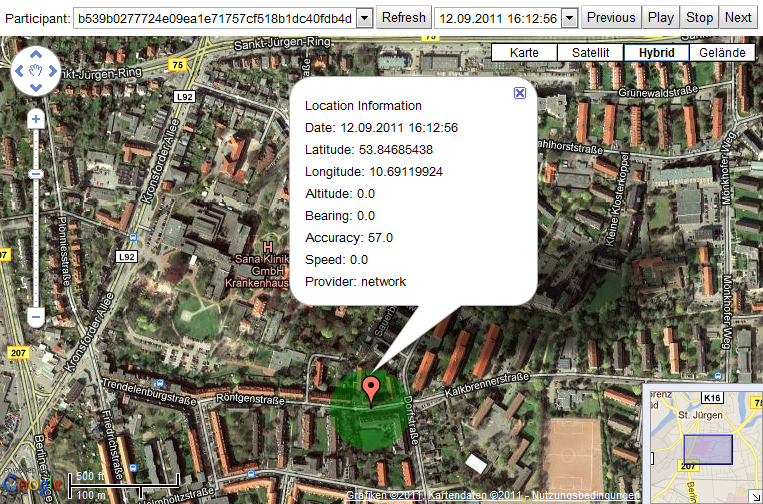
\includegraphics[width=13cm]{grafiken/locationtracker-remote_map.png}
	\caption{Location-Tracker-Datenvisualisierung}
	\label{locationtrackermap}
\end{figure}

Um die Web-Anwendung auf dem eigenen Computer zu starten, muss die {\em
persistence.xml} an die eigene Datenbank angepasst werden. Dann kann
Folgendes auf der Kommandozeile im {\em mdcf-locationtracker-remote}-Verzeichnis
ausgef�hrt werden.

\begin{lstlisting}[language=bash]
mvn gwt:run
\end{lstlisting}

Daraufhin startet der \acs{gwt} eigene Webserver sowie das
Servlet zum Empfang der Daten. Gibt man die entsprechende lokale IP-Adresse innerhalb der
Plug-In-Konfiguration an, so kann der Webserver die Daten vom {\em Mobile Data
Collector} empfangen und �ber die Web-Anwendung darstellen.

\section{Plug-In zum Sammeln der Lautst�rke an der aktuellen Position}
Aufbauend auf dem in Abschnitt \ref{locationtracker} beschriebenen {\em
Location Tracker}, wird im Folgenden ein Plug-In entwickelt, das neben der
aktuellen Position auch die Lautst�rke speichert. Das Plug-In tr�gt den
Arbeitstitel {\em Noise Tracker}.

\subsection{Anpassung des Plug-Ins}
Das Plug-In befindet sich im {\em NoiseTrackerPlugin}-Verzeichnis. Es wird sich
im Folgenden auf dem im Verzeichnis befindlichen Quellcode bezogen.

Da der {\em Location Tracker} bereits die aktuelle Position bestimmt, muss noch
die aktuelle Lautst�rke ermittelt werden. Das ist in Listing \ref{messurenoise}
dargestellt.

\begin{lstlisting}[label=messurenoise,
caption=Lautst�rkenmessung, language=java] 
recorder = new MediaRecorder();
recorder.setAudioSource(MediaRecorder.AudioSource.MIC);
recorder.setOutputFormat(MediaRecorder.OutputFormat.THREE_GPP);
recorder.setAudioEncoder(MediaRecorder.AudioEncoder.AMR_NB);
recorder.setOutputFile("/dev/null");
recorder.prepare();
recorder.start();

double amplitude = 0.0;
for (int i = 0; i < 10; i++) {
	amplitude = getAmplitude();
	Thread.sleep(100);
}

recorder.stop();
recorder.release();
\end{lstlisting}

In dem Listing wird zuerst ein {\em MediaRecorder} erstellt. Dieser kann dazu
verwendet werden, Audio- und Videoaufnahmen durchzuf�hren. In den darauf folgenden
Zeilen wird als Audioquelle das Mikrofon verwendet. Die Einstellungen zum
Ausgabeformat und Audio-Encoder sind zwar notwendig, aber
irrelevant, da, wie in Zeile 5 angegeben, alle Daten im {\em null-Device}
gespeichert werden. Durch die {\em prepare}- und {\em start}-Methode wird das Mikrofon reserviert
und die Aufnahme gestartet. Die Lautst�rke wird nun anhand der maximalen Amplitude
bestimmt, welchen �ber die {\em getAmplitude}-Methode abgefragt werden kann.
Damit die Methode einen brauchbaren Wert zur�ckliefert, muss f�r eine bestimmte
Zeitspanne eine Tonaufnahme erfolgen. In diesem Fall werden f�r eine Sekunde
lang, alle Umgebungsger�usche aufgenommen und die maximale Amplitude bestimmt.
Durch die {\em stop}- und {\em release}-Methode wird die Aufnahme angehalten und das
Mikrofon wieder freigegeben. Diese Art zur Lautst�rkenbestimmung wurde dem
Beispielprogramm {\em NoiseAlert} entnommen~\cite{noisealert}. Hierbei ist darau
hinzuweisen, dass die maximale Amplitude zwischen verschiedenen Ger�ten
variieren kann. Bei einer Auswertung ist deswegen eine Normalisierung der Daten
erforderlich.

Um die Amplitude zum bisherigen Datenmodell hinzuzuf�gen, ist die Zeile
aus Listing \ref{storeamplitude} hinzuzuf�gen.

\begin{lstlisting}[label=storeamplitude,
caption=Speichern der Ampltiude, language=java] 
node.setProperty("Amplitude", amplitude);
\end{lstlisting}

Als letzte Anpassung muss das Plug-In noch die {\em Permission} zur Aufnahme von
Tonaufnahmen erhalten. Dazu muss die {\em AndroidManifest.xml} um die Zeile aus 
Listing \ref{recordaudio} erg�nzt werden.

\begin{lstlisting}[label=recordaudio,
caption=Permission f�r Tonaufnahmen, language=xml] 
<uses-permission
	android:name="android.permission.RECORD_AUDIO" />
\end{lstlisting}

Bei der Verwendung der {\em Permission} sei darauf hingewiesen, dass der
Benutzer wie in Abbildung \ref{activation_recordaudio_warning} eine Warnung bei der
Aktivierung erh�lt, da durch die Aufnahme von Ton personenbezogene Daten erhoben
werden k�nnen. Der {\em Mobile Data Collector} ist nicht in der Lage zu
protokollieren, was wann aufgenommen wurde, sondern kann nur das Resultat
speichern. Siehe hierzu auch Abschnitt \ref{problemsofimplementation}.

\begin{figure}[h!] 
	\centering
	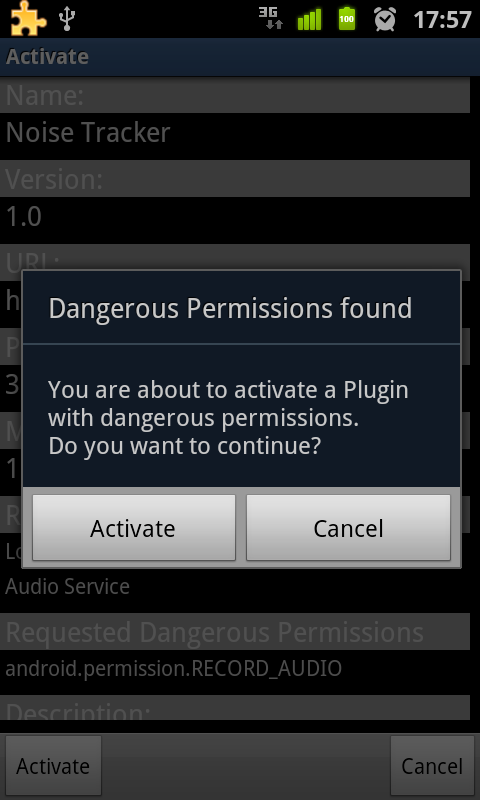
\includegraphics[width=5cm]{grafiken/activation_warning.png}
	\caption{Warnung bei der Aktivierung}
	\label{activation_recordaudio_warning}
\end{figure}

Das Plug-In ist jetzt vollst�ndig implementiert und kann zur Ermittlung der
Lautst�rke verwendet werden.

\subsection{Anpassungen der Serverkomponente}
Die Anpassungen an der Serverkomponente sind ebenfalls gering. Bei
der �ber\-tra\-gung des allgemeinen Datenmodells auf das dom�nenspezifische muss
ein entsprechendes Attribut f�r die Amplitude vorgesehen werden.

Bei der Visualisierung wurde in diesem Fall nur ein weiteres Attribut bei der
Ausgabe aller Positionsdaten hinzugef�gt. Siehe hierzu Abbildung
\ref{noisetrackermap}.

\begin{figure}[h!] 
	\centering
	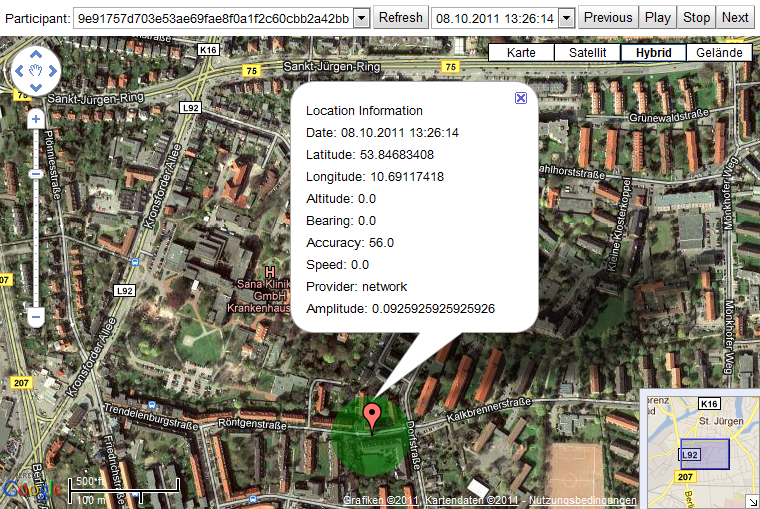
\includegraphics[width=13cm]{grafiken/noisetracker-remote_map.png}
	\caption{Noise-Tracker-Datenvisualisierung}
	\label{noisetrackermap}
\end{figure}

\section{Evaluationsergebnisse}
Als Ergebnis der Evaluation l�sst sich folgendes Festhalten:

\begin{itemize}
  \item Die Erstellung von Plug-Ins f�r reale Anwendungsszenarien, z.~B. die
  Erfassung der aktuellen Positionen und Lautst�rke, ist
  mit dem {\em Mobile Data Collection Framework} m�glich.
  \item Das allgemeine Datenformat erlaubt das Speichern von beliebigen
  Informationen und schr�nkt einen Plug-In-Entwickler nur bedingt ein.
  \item Bestehende Plug-Ins lassen sich leicht an neuen Anforderungen anpassen
  bzw. erweitern.
  \item Bei der Verwendung von Android-{\em Permissions}, die den Zugriff auf
  personenbezogene Daten erm�glichen, wird der Benutzer vor der Aktivierung
  gewarnt.
  \item Die Zugriffe auf die sicheren {\em Android System Services} werden
  protokolliert und sind, wie die vom Plug-In gesammelten Daten, zu jedem
  Zeitpunkt einsehbar.
  \item Die gesammelten Daten lassen sich anonym an externe Server �bertragen
  und persistieren. Die serverseitige Persistenzart ist frei w�hlbar.
  \item Die Visualisierung hat gezeigt, dass die Daten auch verwertbar sind. Der
  Visualisierung sind hierbei keine Grenzen gesetzt.
  \item Es ist zurzeit nicht m�glich, die Aufnahme von Ton und Video �ber den
  {\em Mobile Data Collector} zu protokollieren. Der Benutzer wird aber gewarnt,
  sollte ein Plug-In dieses versuchen.
\end{itemize}

Abschlie�end l�sst sich festhalten, dass die in der Anforderungsanalyse und dem
Konzept definierten Anforderungen fast vollst�ndig realisiert wurden, mit
Ausnahme der Protokollierung beim Zugriff auf Ton- und Videodaten.
	\chapterfin
	\chapter{Zusammenfassung und Ausblick}
\label{cha:zusammenfassung}
Im Rahmen dieser Masterarbeit wurde ein Softwaresystem entwickelt, das eine
vertrauensw�rdige Plattform darstellen kann, von der Benutzer und Entwickler
gleicherma�en profitieren k�nnen. Der Benutzer erh�lt eine Anwendung, mit der er
mehr M�glichkeiten hat zur informationellen Selbstbestimmung. Er kann selbst
entscheiden, wann, welche Daten, er wem freigeben m�chte und kann der Freigabe
auch widersprechen. Der Entwickler im Gegenzug erh�lt eine Plattform, auf der er
Anwendungen zum Sammeln von Sensordaten entwickeln kann, ohne sich selbst um das
Thema Transparenz k�mmern zu m�ssen. Das kann Zeit und somit auch Geld sparen.
Auch kann er das m�gliche Vertrauen, welches in das System gesetzt wird, auf
seine Anwendung �bertragen. Ein Benutzer ist dadurch eher gewillt, eine f�r die
Plattform entwickelte Anwendung zu verwenden, die personenbezogene Daten
sammelt.

Das entwickelte Softwaresystem besteht aus zwei Teilen. Der erste Teil besteht
aus einer Android Anwendung, dem {\em Mobile Data Collector}, welche der
Benutzer auf seinem Smartphone installiert und verwendet. Der andere Teil
beinhaltet ein Rahmenwerk mit dem Entwickler Erweiterungen bzw. Plug-Ins zum
Sammeln von Daten, f�r den {\em Mobile Data Collector} entwickeln k�nnen.

Der {\em Mobile Data Collector} erlaubt durch seine grafische Oberfl�che die
einfache Verwaltung von Plug-Ins. Der Benutzer kann Plug-Ins aktivieren und
deaktivieren und kann somit entscheiden, wann Daten �ber ihn gesammelt werden
sollen. Des Weiteren kann er �ber die grafische Oberfl�che zu jedem Zeitpunkt
einsehen, welche Daten �ber ihn angefordert und letztendlich gesammelt wurden.
Dazu werden m�glichst viele Aktivit�ten des Plug-Ins protokolliert. War ein
Plug-In f�r eine bestimmte Zeitspanne aktiv und m�chte seine Daten �bertragen,
so kann der Benutzer vor der �bertragung entscheiden, ob er die gesammelten
Daten freigeben will oder nicht. Er kann auch die �bertragung beliebig
verz�gern, um den �bertragungszeitpunkt selbst w�hlen zu k�nnen. Dadurch kann
bei der Verwendung mobiler Datenverbindungen Geld bzw. Datenvolumen gespart
werden. Gefahren, die von einem Plug-In ausgehen k�nnten, werden dem Benutzer
vor der ersten Aktivierung angezeigt. Dadurch soll der Schaden der durch die
Ausf�hrung eines Plug-Ins entstehen kann minimiert werden.

Das Rahmenwerk f�r Entwickler besteht selbst auch aus zwei Komponenten. Zum
einem aus dem {\em Mobile Data Collection Framework}, das zur Entwicklung von
Plug-Ins verwendet wird sowie einem serverseitigen Framework zum Empfang der
gesammelten Daten. Die Frameworks erlauben die einfache Entwicklung von
Anwendungen zum Sammeln von Sensordaten und einer dazugeh�rigen
Serverkomponente, um die Daten vom {\em Mobile Data Collector} zu empfangen.

Um die Anonymit�t des Benutzers zu sch�tzen, wird der Zugriff auf eindeutige
Benutzerdaten durch den {\em Mobile Data Collector} erschwert. Um aber eine
Zuordnung zwischen einzelnen Datens�tzen auf dem Server zu erm�glichen, stellt
der {\em Mobile Data Collector} eine anonyme eindeutige Benutzerkennung bereit.

Im Rahmen der Evaluation wurde anhand eines Plug-Ins zur Positionsverfolgung
gezeigt, dass sich mit dem {\em Mobile Data Collection Framework} Plug-Ins f�r
reale Anwendungsszenarien entwickeln lassen. So ist die Aufnahme von
Positionsdaten (die wohl wichtigste Art von Daten im Bereich der mobilen
Datenerfassung) relativ einfach m�glich. Auch l�sst sich das Plug-In einfach um
die Erfassung zus�tzlicher Daten erweitern. In diesem Fall um die aktuelle
Umgebungslautst�rke. Hierbei wurde bewusst darauf geachtet, den Entwickler so
wenig wie m�glich bei der Entwicklung von Plug-Ins einzuschr�nken. Die
Evaluation zeigt aber auch die zurzeit bestehenden �berwachungsgrenzen des {\em
Mobile Data Collectors}. So ist eine Protokollierung von Zugriffen auf die
Kamera und das Mikrofon nicht bzw. nur mit relativ gro�em Aufwand m�glich.
Das Problem l�sst sich am besten durch den Einsatz des \acs{osgi}-Frameworks
l�sen. Hierbei bleibt abzuwarten bis Frameworks wie Dynamix den n�tigen Reifegrad
erreicht haben, um diese im produktiven Einsatz zu verwenden.

Das zuk�nftige Anwendungsgebiet des {\em Mobile Data Collector} liegen in
erster Linie im Bereich der Forschung. Hier existiert eine Vielzahl von
Projekten, die auf die Erhebung von personenbezogenen Daten angewiesen sind.

	\chapterfin

%---------------------------------------------------------------------------
% Anhang
%---------------------------------------------------------------------------
	\appendix
		
		%---------------------------------------------------------------------------

	\addcontentsline{toc}{chapter}{Verzeichnisse}

		%---------------------------------------------------------------------------
		\addcontentsline{toc}{section}{Abbildungsverzeichnis}
		\listoffigures
		\sectionfin		
		%---------------------------------------------------------------------------
	
		%---------------------------------------------------------------------------
		%\addcontentsline{toc}{section}{Abk�rzungsverzeichnis}
		%If you are using e. g. the documentclass book with page style headings you
		%should also take care of correct headings:	
		%\markboth{Abk�rzungsverzechnis}{Abk�rzungsverzechnis}
		%\printnomenclature
		%\sectionfin
		%Abk�rzungsverzeichnis
		
		%\phantomsection
		\addcontentsline{toc}{section}{Abk�rzungsverzeichnis}
		\markboth{Abk�rzungsverzechnis}{Abk�rzungsverzechnis}
		\section*{Abk�rzungsverzeichnis}
		\begin{acronym}[MMORPG]
			\setlength{\itemsep}{-\parsep}
			\renewcommand{\bflabel}[1]{\normalfont{\normalsize{\textbf{#1}}}\hfill}
			\acro{aidl}[AIDL]{Android Interface Definition Language}
\acro{api}[API]{Application Programming Interface}
\acro{db4o}[db4o]{database for objects}
\acro{gps}[GPS]{Global Positioning System}
\acro{gsm}[GSM]{Global System for Mobile Communications}
\acro{gwt}[GWT]{Google Web Toolkit}
\acro{http}[HTTP]{Hypertext Transfer Protocol}
\acro{ide}[IDE]{Integrated Development Environment}
\acro{idl}[IDL]{Interface Definition Language}
\acro{imsi}[IMSI]{International Mobile Subscriber Identity}
\acro{ipc}[IPC]{Inter Process Communication}
\acro{itm}[ITM]{Institut f�r Telematik}
\acro{lan}[LAN]{Local Area Network}
\acro{jar}[JAR]{Java Archive}
\acro{jcr}[JCR]{Java Content Repository}
\acro{json}[JSON]{Java Script Object Notation}
\acro{jsr}[JSR]{Java Specification Request}
\acro{orm}[ORM]{Objekt Relationale Mapper}
\acro{osgi}[OSGi]{Open Services Gateway initiative}
\acro{rest}[REST]{Representational State Transfer}
\acro{sql}[SQL]{Structured Query Language}
\acro{qbe}[QBE]{Query By Example}
\acro{pojo}[POJO]{Plain Old Java Object}
\acro{sdk}[SDK]{Software Development Kit}
\acro{sha}[SHA]{Secure Hash Algorithm}
\acro{umts}[UMTS]{Universal Mobile Telecommunications System}
\acro{vm}[VM]{Virtual Machine}
\acro{xml}[XML]{Extensible Markup Language}
		\end{acronym}
		\sectionfin
		%---------------------------------------------------------------------------
	
		%---------------------------------------------------------------------------
		%---------------------------------------------------------------------------
		\renewcommand\bibname{Bibliographie}
		\addcontentsline{toc}{section}{Bibliographie}
		\bibliographystyle{acm}
		\bibliography{quellen/master}

		\chapterfin

\end{document}
